\documentclass[11pt,a4paper]{article}
\usepackage{fontspec}
\usepackage{amsmath,amssymb,amsthm}
\usepackage{unicode-math}
\usepackage[a4paper,margin=25mm]{geometry}
\usepackage{booktabs,longtable,tabularx,array}
\usepackage{enumitem}
\usepackage{xcolor}
\usepackage{graphicx}
\usepackage{tikz}
\usetikzlibrary{arrows.meta,positioning,fit,calc}
\usepackage{hyperref}
\usepackage[nameinlink,noabbrev]{cleveref}

\defaultfontfeatures{Ligatures=TeX}
\setmainfont{TeX Gyre Pagella}
\setsansfont{TeX Gyre Heros}
\setmonofont{Latin Modern Mono}[Scale=MatchLowercase]
\setmathfont{TeX Gyre Pagella Math}

\definecolor{provedcolor}{HTML}{176B45}
\definecolor{partialcolor}{HTML}{9A6700}
\definecolor{specifiedcolor}{HTML}{315E9E}
\definecolor{blockedcolor}{HTML}{A43A3A}
\definecolor{deferredcolor}{HTML}{6B4FA1}
\definecolor{ink}{HTML}{1E293B}
\definecolor{softgray}{HTML}{F3F4F6}
\definecolor{analogycolor}{HTML}{0F766E}

\hypersetup{
  colorlinks=true,
  linkcolor=specifiedcolor,
  citecolor=provedcolor,
  urlcolor=specifiedcolor,
  pdftitle={An Algebraic Map of HAETAE-2 Implementation Verification},
  pdfsubject={A HAETAE top-down EasyCrypt guide for pure algebraists and algebraic geometers},
  pdfauthor={HAETAE top-down EasyCrypt project}
}

\setlist[itemize]{leftmargin=2em,itemsep=0.28em,topsep=0.4em}
\setlist[enumerate]{leftmargin=2.3em,itemsep=0.28em,topsep=0.4em}
\renewcommand{\arraystretch}{1.18}
\renewcommand{\contentsname}{Contents}
\renewcommand{\figurename}{Figure}
\renewcommand{\tablename}{Table}
\renewcommand{\refname}{References}
\setlength{\emergencystretch}{5em}
\setlength{\parindent}{1em}
\setlength{\parskip}{0.18em}

\newcolumntype{Y}{>{\raggedright\arraybackslash}X}
\newcolumntype{L}[1]{>{\raggedright\arraybackslash}p{#1}}

\theoremstyle{definition}
\newtheorem{definition}{Definition}[section]
\newtheorem{translation}[definition]{Translation principle}
\newtheorem{verified}[definition]{Verified proposition}
\newtheorem{openobligation}[definition]{Open obligation}
\newtheorem{caution}[definition]{Caution}
\newtheorem{question}[definition]{Participation question}

\crefname{definition}{Definition}{Definitions}
\crefname{translation}{Translation principle}{Translation principles}
\crefname{verified}{Verified proposition}{Verified propositions}
\crefname{openobligation}{Open obligation}{Open obligations}
\crefname{caution}{Caution}{Cautions}
\crefname{question}{Participation question}{Participation questions}

\newcommand{\identifier}[1]{\nolinkurl{#1}}
\newcommand{\sourcepath}[1]{\nolinkurl{#1}}
% EasyCrypt declarations are long and underscore-heavy.  Use the same
% proportional font as the surrounding text so long identifiers can wrap
% without consuming table width like typewriter text.
\newcommand{\theoremname}[1]{{\begingroup\urlstyle{same}\nolinkurl{#1}\endgroup}}
\newcommand{\claimid}[1]{\textsf{\textbf{\detokenize{#1}}}}
\newcommand{\statusproved}{\textcolor{provedcolor}{\textsf{\textbf{PROVED}}}}
\newcommand{\statuspartial}{\textcolor{partialcolor}{\textsf{\textbf{PARTIAL}}}}
\newcommand{\statusspecified}{\textcolor{specifiedcolor}{\textsf{\textbf{SPECIFIED}}}}
\newcommand{\statusblocked}{\textcolor{blockedcolor}{\textsf{\textbf{BLOCKED}}}}
\newcommand{\statusdeferred}{\textcolor{deferredcolor}{\textsf{\textbf{DEFERRED}}}}

\newcommand{\ZZ}{\mathbb{Z}}
\newcommand{\FF}{\mathbb{F}}
\newcommand{\BB}{\mathbb{B}}
\newcommand{\Rq}{R_q}
\newcommand{\Bytes}{\mathsf{Byte}}
\newcommand{\Mem}{\mathsf{Mem}}
\newcommand{\take}{\mathop{\mathrm{take}}}
\newcommand{\prefix}{\mathop{\mathrm{prefix}}}
\newcommand{\restrict}{\mathord{\upharpoonright}}
\newcommand{\Encode}{\mathop{\mathrm{Enc}}}
\newcommand{\Decode}{\mathop{\mathrm{Dec}}}
\newcommand{\obs}{\mathop{\mathrm{obs}}}
\newcommand{\Adv}{\mathop{\mathrm{Adv}}}

\newenvironment{takeaway}[1]
  {\begin{quote}\color{ink}\noindent\textbf{#1}\par\smallskip}
  {\end{quote}}

\newenvironment{analogy}
  {\begin{quote}\color{analogycolor}\noindent\textbf{Analogy (not a formalized theorem).}\par\smallskip}
  {\end{quote}}

\tikzset{
  layernode/.style={
    draw=specifiedcolor,
    rounded corners=2pt,
    fill=specifiedcolor!6,
    align=center,
    minimum height=11mm,
    text width=35mm,
    inner sep=4pt
  },
  provennode/.style={
    draw=provedcolor,
    rounded corners=2pt,
    fill=provedcolor!7,
    align=center,
    minimum height=11mm,
    text width=38mm,
    inner sep=4pt
  },
  partialnode/.style={
    draw=partialcolor,
    dashed,
    rounded corners=2pt,
    fill=partialcolor!7,
    align=center,
    minimum height=11mm,
    text width=38mm,
    inner sep=4pt
  },
  blockednode/.style={
    draw=blockedcolor,
    dashed,
    rounded corners=2pt,
    fill=blockedcolor!5,
    align=center,
    minimum height=11mm,
    text width=38mm,
    inner sep=4pt
  },
  deferrednode/.style={
    draw=deferredcolor,
    densely dotted,
    rounded corners=2pt,
    fill=deferredcolor!6,
    align=center,
    minimum height=11mm,
    text width=38mm,
    inner sep=4pt
  },
  flowarrow/.style={-{Latex[length=2.2mm]},thick,draw=ink},
  openarrow/.style={-{Latex[length=2.2mm]},thick,dashed,draw=partialcolor}
}

% Snapshot metadata.  The 82-target paper surface remains frozen; the current
% branch also carries explicitly separated post-freeze EasyCrypt evidence.
\newcommand{\SnapshotDate}{13 August 2026}
\newcommand{\SnapshotWeek}{Post-PAPER--FREEZE faithful augmented KeyGen coefficient-product composition}
\newcommand{\AuthoredTargetCount}{82}
\newcommand{\WeekTenTargetCount}{6}
\newcommand{\WeekElevenTargetCount}{7}
\newcommand{\WeekTwelveTargetCount}{8}
\newcommand{\WeekThirteenTargetCount}{2}
\newcommand{\WeekFourteenTargetCount}{5}
\newcommand{\WeekFifteenTargetCount}{2}
\newcommand{\WeekSixteenTargetCount}{8}
\newcommand{\FrozenPaperGate}{\identifier{STOP-VERIFY-MATRIX-CRT}}
\newcommand{\CurrentGate}{\identifier{STOP-KG-AVEC-QJ}}
\newcommand{\FaithfulAugmentedVerdict}{\identifier{GO-KG-FAITHFUL-AUGMENTED}}
\newcommand{\CurrentPriority}{\claimid{OBL-KG-SECURITY-EXPANDVECA-SEMANTICS}: a theorem replacing/refining synthetic security ExpandVecA with actual SHAKE128/rejection semantics}
\newcommand{\ProjectMode}{HAETAE-2}


\title{\textbf{An Algebraic Map of HAETAE-2 Implementation Verification}\\[0.4em]
  \Large A Companion Guide for Pure Algebraists and Algebraic Geometers}
\author{HAETAE top-down EasyCrypt working document}
\date{Status as of: \SnapshotDate\ (\SnapshotWeek)}

\begin{document}
\maketitle

\begin{abstract}
HAETAE-2 is a module-lattice signature over
\(R_q=\ZZ_q[X]/(X^{256}+1)\).
The objects actually proved about in this repository, however, extend beyond
the ring itself. Elements and module maps from the paper are represented as
canonical byte strings, those strings are placed in finite memory, and the
proofs descend to the fact that actual generated Jasmin procedures preserve
or invert those representations. This guide organizes that process into three
layers: algebraic objects, representation maps, and state-machine refinement.

At the snapshot serving as the latest audit baseline, \AuthoredTargetCount\
authored EasyCrypt targets were included in the frozen manifest and passed
an aggregate \identifier{-no-eco} fresh compile. Post-freeze standalone
theories are not included in that count.
After the \WeekTenTargetCount\ Week~10 rANS encoder targets came
\WeekElevenTargetCount\ Week~11 encoder-closure targets,
\WeekTwelveTargetCount\ Week~12 decoder semantic-refinement targets,
\WeekThirteenTargetCount\ Week~13 actual-core-composition targets,
\WeekFourteenTargetCount\ Week~14 production full-HBZ boundary targets,
\WeekFifteenTargetCount\ Week~15 fixed all-6 success targets, and
\WeekSixteenTargetCount\ Week~16 MINCORE KeyGen/KG--NTT boundary and
Sign/Verify control/word targets.
The completed core covers the secret key's 992-byte verification-key prefix,
agreement of the 32-byte \(\mu\) between raw/internal Sign and Verify,
challenge-suffix absorption, the signature-prefix round trip, HBZ
coefficient--symbol leaf inverses, certificates for the actual 13-symbol rANS
table, pure rANS step and byte-stack theorems, actual suffix copying,
encoder--decoder harness control, and the exact equality between the entire
successful output of the actual encoder and pure
\(\operatorname{TraceBytes}(\operatorname{SymbolList}(symbols_0))\).
It also includes refinement of the actual decoder recovering 1024 symbols from
an exact trace, the core inverse composing those two theorems and actual suffix
copying in \identifier{Mode2RansActualHarness.run}, and the production full-HBZ
wrapper inverse lifting actual
\identifier{_encode_hb_z1_full}/\identifier{_decode_hb_z1_full}
to the SignaturePack/Unpack boundary. Week~15 excludes actual failure for the
all-6 stream generated by canonical all-zero HBZ and proves \(bad=0\),
\(4\le size\le1024\), exact trace/frame, and the production zero round trip
for executions that return. This is fixed-input Hoare partial correctness,
not termination, losslessness, or probability-1 success.

For a snapshot that calls actual \identifier{_kp_m23_matrix} and
\identifier{_keypair_finalize_m23} consecutively, Week~16 established
\(r=2b_1+b_0\), \(b_0\in[-1,1]\), adjusted \(s_2=s_2-b_0\), and a
snapshot-only zero congruence mod \(2q\). However, even after actual
\theoremname{output_row_from_mode2_ntt_words} fixed \identifier{output_row}
to the actual full-invNTT/pointwise representation, the full-NTT convolution
theorem and representation adapter needed to transfer it to a native \(R_q\)
product and the security model's \(A_{\mathrm{gen}}s_{\mathrm{gen}}\) product
were absent at the frozen-paper stage. KeyGen was therefore frozen at
KG-2/finalization under \identifier{STOP-KG-NTT}. Direct actual-call/control
results for the accepted Sign core then compiled, and a partial MINCORE-VERIFY
theorem was added at the canonical decoded \((x,v,h,c)\) boundary:
V-1/V-2/V-5/V-6, the W64 norm gate, and tail-trace/mismatch word expressions
remain proved, with explicit matrix and challenge blockers.
The frozen-paper verdict is \FrozenPaperGate.

Post-freeze proofs completed the pure full-NTT spectral action, native \(R_q\)
row product, and \(R_q\)--HAETAE dot-product representation transport, and
interpreted actual \identifier{avec} expansion as the paper's \(a\).
The paper's \(qj\) term was independently composed into the snapshot congruence.
However, the existing security-side \identifier{haetae_mode23_qj_vector} is a
synthetic generator, and concrete coefficients were proved to differ from the
paper's \(qj\) and actual SHAKE128/rejection expansion.
The current verdict is \CurrentGate, with
\claimid{OBL-KG-SECURITY-EXPANDVECA-SEMANTICS} as the first repair obligation.
The second \(h\) suffix codec, complete signature codec, product/replay transport
connecting stored \(\mu\) in completed API traces, full functional correctness,
and implementation-level security also remain open. This guide does not declare
a complete proof; it marks exactly which parts of the commuting diagram have
been closed.

The latest post-freeze \sourcepath{KgFaithfulAugmentedModel.ec} also passes
standalone fresh compilation. It instantiates a width-6 carrier with the actual
matrix/secret and defines a structured coefficient product by transporting the
generated 3-term row product to HAETAE \identifier{poly_dot}.
\theoremname{actual_faithful_augmented_productE} expands this product on active
rows, while
\theoremname{checked_mode2_parent_m23_finalize_faithful_augmented_paper_as_qj}
shows, at every active coefficient, its congruence with faithful (qj) mod-(2q).
The product takes only the matrix and secret as inputs, reconstructs the middle
2-by-3 block from their columns, and evaluates it with \identifier{poly_dot}.
The verdict for this work is therefore \FaithfulAugmentedVerdict.
Its mod-\(2q\) block-specific semantics nevertheless differ from the existing
mod-\(q\), width-4 security \identifier{matrix_vec_mul}; agreement with the
synthetic security object is not a conclusion. This separate closure therefore
changes neither the frozen target count nor the current security gate.
\end{abstract}

\begin{takeaway}{One-sentence summary}
The current results establish that several deterministic representation squares
of the signature scheme commute down to actual generated code; they do not mean
that the entire signature scheme over the ring has already been verified.
The next central gate is
\claimid{OBL-KG-SECURITY-EXPANDVECA-SEMANTICS}, replacing/refining synthetic
security ExpandVecA to agree with actual SHAKE128/rejection semantics.
Week~15's fixed all-6 failure exclusion is \statusproved\ but gives no
termination result. The KG-2-like decomposition, snapshot congruence, and final
NTT-word representation rewrite at Week~16's actual KeyGen snapshot/finalizer
boundary are complete. The full-NTT convolution/representation adapter missing
from the frozen paper was completed post-freeze, but revealed a later obstacle:
actual \identifier{avec}, the paper's \(qj\), and the synthetic security object
cannot be identified. The current verdict is therefore \CurrentGate, without
overwriting the frozen-paper verdict \FrozenPaperGate. This is not a verdict
of completed full KeyGen, \(h\) codec, full signature codec, or Sign--Verify
correctness.
\end{takeaway}

\tableofcontents
\clearpage

\section{Reading contract and overall map}
\label{sec:reading-contract}

\subsection{What this guide assumes and explains}

This guide assumes familiarity with rings, quotient rings, free modules,
equivalence relations and quotient sets, commutative diagrams, and induction.
It uses standard English mathematical terminology in introductions, headings,
figures, and the glossary, with consistent terms in repeated contexts.
It does not assume knowledge of the following.

\begin{itemize}
  \item The design of HAETAE or module-lattice signatures;
  \item Jasmin syntax and memory models;
  \item EasyCrypt's Hoare logic, pRHL, or tactic language;
  \item Implementation conventions for rANS entropy coding.
\end{itemize}

The goal is not a line-by-line explanation of every source file.
For each proof obligation, the guide asks: “What is the object?”,
“Which map must commute?”, “Which premises restrict its domain?”,
and “Which arrows have currently been proved for actual procedures?”
The project's scope is limited to mode~2 and pinned specification/implementation
snapshots \cite{project-scope}.

\begin{translation}[Translation across three layers]
Read the repository's theorems as propositions moving between three layers.
\begin{enumerate}
  \item \textbf{Algebraic layer}: \(R_q\)-module elements, decompositions,
        challenges, and paper algorithms;
  \item \textbf{Representation layer}: canonical byte strings, prefix
        projections, memory regions, and fixed-width integers;
  \item \textbf{Execution layer}: actual generated procedures, branches,
        loops, return values, and trace observations.
\end{enumerate}
Transporting an equality from one layer to another always requires a named
representation/refinement theorem. A shared mathematical intention does not
make a diagram commute automatically.
\end{translation}

\begin{figure}[ht]
\centering
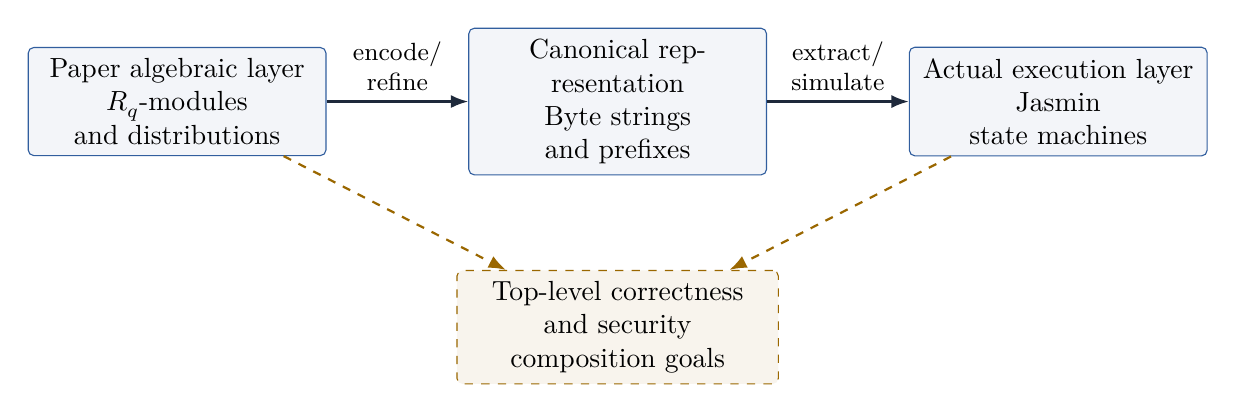
\begin{tikzpicture}[node distance=8mm and 18mm]
  \node[layernode] (alg) {Paper algebraic layer\\\(R_q\)-modules\\and distributions};
  \node[layernode, right=of alg] (repr) {Canonical representation\\Byte strings\\and prefixes};
  \node[layernode, right=of repr] (proc) {Actual execution layer\\Jasmin\\state machines};
  \node[partialnode, below=12mm of repr] (security) {Top-level correctness\\and security\\composition goals};
  \draw[flowarrow] (alg) -- node[above,align=center,font=\small]{encode/\\refine} (repr);
  \draw[flowarrow] (repr) -- node[above,align=center,font=\small]{extract/\\simulate} (proc);
  \draw[openarrow] (proc) -- (security);
  \draw[openarrow] (alg) -- (security);
\end{tikzpicture}
\caption{Overall proof structure. Only some horizontal arrows are closed;
the top-level composition arrows remain partial.}
\label{fig:three-layers}
\end{figure}

\subsection{Status terms include logical quantifiers}

The operational source of truth is \sourcepath{CLAIM_LEDGER.md}
\cite{claim-ledger}; dependencies are recorded in
\sourcepath{THEOREM_GRAPH.md} \cite{theorem-graph}.
This guide uses status terms only with the following meanings.

\begin{center}
\begin{tabularx}{\textwidth}{L{28mm} Y Y}
\toprule
Status & Exact meaning & What does not follow automatically \\
\midrule
\statusproved & A named EasyCrypt declaration freshly compiles under the stated premises. &
Parent claims, termination, losslessness, distributional equality \\
\statuspartial & Child propositions or restricted directions are proved, but the named parent remains open. &
A global statement with the restrictions removed \\
\statusspecified & Operations, predicates, or interfaces expressing the goal compile. &
A proof of the goal \\
\statusblocked & A specific extraction, semantic, numerical, or probabilistic theorem is missing, preventing composition. &
A claim that the obstacle is insurmountable \\
\statusdeferred & Explicitly frozen at a paper boundary after a time limit. &
A claim that the obligation is false or unnecessary \\
\bottomrule
\end{tabularx}
\end{center}

In particular, “Hoare partial correctness is proved” means
\[
  \text{if the procedure returns, the postcondition holds}
\]
rather than that the procedure returns on every input or that a probabilistic
retry terminates almost surely. This distinction is essential because of
KeyGen and Sign rejection loops.

\subsection{How far algebraic geometry applies}

The ring \(R_q\) of course defines the affine scheme
\(\operatorname{Spec}R_q\). Local memory restrictions, local equalities,
and frame conditions also suggest restriction maps and gluing.
The current EasyCrypt files, however, do not formalize schemes, varieties,
spectra, sheaves, or cohomology. Proofs chiefly concern arrays over finite sets,
fixed-width words, state transitions, and integer division.

\begin{analogy}
Viewing memory \(m\) as a section over an address set, and equality on a region
\(U\) as \(m_1\restrict_U=m_2\restrict_U\), quickly suggests the shape of
region-local hash theorems. The analogy does not use sheaf axioms or a scheme
structure to derive EasyCrypt conclusions. The actual basis is pointwise
\identifier{load8} equality and the procedure's read footprint.
\end{analogy}

Algebraic geometers should pay particular attention to hashes.
SHAKE state transitions are generally neither \(R_q\)-linear maps nor regular
morphisms. This guide treats hashing as a deterministic state machine reading
finite byte strings. Equality of hash inputs therefore yields equality of
outputs through relational execution theorems about the two actual programs,
rather than through algebraic functionality.

\subsection{Six statements to remember first}

\begin{enumerate}
  \item Top-level \identifier{FC_KeyGen}, \identifier{FC_Sign}, and
        \identifier{FC_Verify} are still goal interfaces, not completed theorems.
  \item \(\prefix_{992}(sk)=vk\) and raw/internal \(\mu\)-prefix agreement
        are proved down to actual generated procedures, but do not automatically
        establish complete API security.
  \item The pure HBZ/rANS inverse structure, individual actual encoder/decoder
        trace refinements, core-harness inverse including actual copying,
        and production full-HBZ wrapper arrows are closed as
        success-conditioned partial correctness.
  \item For the all-6 stream generated by canonical all-zero HBZ, failure of a
        returning actual encoder is excluded and the production zero round
        trip is proved; fixed-input termination, losslessness, and
        \identifier{phoare} remain open.
  \item The actual KeyGen matrix/finalize snapshot has a proved KG-2-like
        decomposition and snapshot-only mod-\(2q\) congruence. At the frozen-paper
        stage, however, full-NTT convolution and the representation adapter
        following the final \identifier{output_row} NTT-word rewrite were
        absent, so work was frozen under \identifier{STOP-KG-NTT}.
        Sign was subsequently frozen under \identifier{STOP-SIGN-CHAL-MODE2};
        Verify was frozen at \FrozenPaperGate, lacking the actual 2-by-4
        NTT/CRT/freeze procedure
        \cite{week16-sign-report,week16-verify-report}.
        Post-freeze work closed pure convolution, the native \(R_q\) row
        product, and \(R_q\)--HAETAE representation transport, and interpreted
        actual \identifier{avec} as the paper's \(a\).
        But security-side synthetic ExpandVecA differs from actual
        SHAKE128/rejection semantics and the paper's \(qj\), so the current
        status is \CurrentGate. This does not change the frozen 82-target
        verdict \cite{post-freeze-kg-rq-haetae-report,
        post-freeze-kg-actual-avec-qj-report,paper-freeze-artifacts}.
  \item Separate final cryptographic assumptions from implementation proof
        obligations. Implementation correctness beyond the MLWE/BST-MSIS/ROM
        interfaces is not hidden as an assumption.
\end{enumerate}

These six statements govern status judgments throughout the following chapters.

\section{Algebraic objects: from quotient rings to signature bytes}
\label{sec:algebraic-object}

\subsection{The base rings and mode~2 parameters}

In the pinned specification,
\[
  R=\ZZ[X]/(X^{256}+1),\qquad
  R_q=\ZZ_q[X]/(X^{256}+1),\qquad q=64513
\]
and the mode~2 module dimensions are \((k,\ell)=(2,4)\).
The small-secret-coefficient bound is \(\eta=1\), and the binary challenge
has Hamming weight \(\tau=58\) \cite{haetae-spec}.
Each \(R_q\) element is an equivalence class of polynomials of degree
\(<256\); choosing coefficient vectors identifies it with \(\ZZ_q^{256}\)
as a set.

The specification chooses \(q\equiv1\pmod{512}\), so \(X^{256}+1\) splits
completely over \(\FF_q\) and an NTT is available.
On paper, one can therefore consider the Chinese remainder theorem isomorphism
\[
  R_q\simeq\prod_{i=1}^{256}\FF_q
\]
The repository's top-level implementation-security interface nevertheless
retains \identifier{obl_public_key_algebra_ntt} as a separate obligation.
Existence of this isomorphism and correctness of actual NTT routines must not
be treated as the same claim.

\begin{caution}[Separate mathematical background from implementation theorems]
The ring/module description in this section explains the pinned HAETAE
specification. The implementation theorem that “actual Jasmin NTT computes
this isomorphism correctly” requires a separate proposition and premises.
This guide applies \statusproved\ only to named theorems under
\sourcepath{easycrypt/}.
\end{caution}

\subsection{Viewing KeyGen as a module map}

In the paper's KeyGen data flow, a seed generates
\(a_{\mathrm{gen}}\in R_q^k\) and
\(A_{\mathrm{gen}}\in R_q^{k\times(\ell-1)}\).
Small elements \(s_{\mathrm{gen}}\in R^{\ell-1}\) and
\(e_{\mathrm{gen}}\in R^k\) are sampled, and
\[
  b=a_{\mathrm{gen}}+A_{\mathrm{gen}}s_{\mathrm{gen}}
      +e_{\mathrm{gen}}\in R_q^k
\]
is computed. The coefficientwise decomposition
\[
  b=b_0+2b_1,\qquad
  (b_0,b_1)=
  (\operatorname{LowBits}_{vk}(b),
   \operatorname{HighBits}_{vk}(b))
\]
then compresses the verification key to \(vk=(\mathit{seedA},b_1)\).
The packed secret-key representation includes those bytes as a prefix so that
Sign can read the same verification-key components.

The first composition seam closed in this repository is this inclusion
relation, not the complete KeyGen distribution.
Let \(S\) be the set of secret-key byte arrays and \(V\) the set of
verification-key arrays, and define
\[
  \pi_{992}:S\longrightarrow \Bytes^{992},\qquad
  \pi_{992}(s)=s[0..992)
\]
For a returning execution of actual mode~2 internal KeyGen with result
\((vk,sk)\),
\[
  \pi_{992}(sk)=\pi_{992}(vk)
\]
The array on the right is larger; only its first 992 bytes are compared.

This can also be expressed precisely as a quotient. Define on \(S\)
\[
  s\sim_{992}s'\quad\Longleftrightarrow\quad
  s[0..992)=s'[0..992)
\]
Then \(\pi_{992}\) classifies \(S/{\sim_{992}}\).
The current theorem states that the \(\sim_{992}\)-equivalence class of the
packed secret key agrees with the public-key representation. It does not
state equality of the entire secret keys.

\subsection{The Week 16 KeyGen snapshot congruence}

Week~16's transparent harness
\identifier{ActualM23MatrixFinalizeSnapshot.run} calls actual
\identifier{_kp_m23_matrix} with mode~2 dimensions \((2,3)\), stores its
returned \(bp\) as \(\mathit{pre\_bp}\), and calls actual
\identifier{_keypair_finalize_m23} on 512 active words
\cite{week16-mincore-plan,week16-kg-report,week16-kg-ntt-mul-report}.
At coefficient \(i\), let
\[
  r_i=(\mathit{pre\_bp}_i+s_{2,i}+a_i)\bmod q
\]
The compiled semantic snapshot gives
\[
  r_i=2b_{1,i}+b_{0,i},\qquad -1\le b_{0,i}\le1,
  \qquad s'_{2,i}=s_{2,i}-b_{0,i}
\]
Moreover,
\[
  2(a_i-2b_{1,i})+2\mathit{pre\_bp}_i+2s'_{2,i}
  \equiv0\pmod{2q}
\]
holds at every active coefficient. Here \(\mathit{pre\_bp}\) is the return
snapshot of the actual matrix helper; it has not yet been identified with
the paper's \(A_{\mathrm{gen}}s_{\mathrm{gen}}\).

\begin{caution}[Separate the snapshot congruence from the paper's KeyGen equation]
\theoremname{actual_m23_matrix_finalize_semantic_snapshot} combines two actual
calls, low/high decomposition, adjusted \(s_2\), and the frame in one Hoare
postcondition.
\theoremname{output_row_from_mode2_ntt_words} identifies
\identifier{KeygenM23ArithmeticSpec.output_row} exactly with the actual
full-invNTT/pointwise word representation.
The frozen paper ended at \identifier{STOP-KG-NTT}, lacking the odd-root
orthogonality/full-NTT convolution theorem and representation adapter needed
to transport that representation to native \(R_q\) negacyclic multiplication.

Post-freeze,
\theoremname{rq_mul_coeff_foldr_to_bigi},
\theoremname{full_ntt_montgomery_spectral_action},
\theoremname{full_ntt_montgomery_row_product},
\theoremname{keygen_mode2_row_product}, and
\theoremname{mode2_row_product_haetae_dot}
close this pure algebra and representation transport.
The two actual \identifier{avec} rows are also interpreted as the paper's
\(a\), and \(qj\) from the paper's \(j=(1,0)^T\) is added as a separate term
in the snapshot congruence.
The existing security-side \identifier{haetae_mode23_qj_vector}, however, is
a synthetic generator starting at coefficient 401, different from the paper's
\(qj[0,0]=64513\) and actual SHAKE128/rejection expansion.
The congruence above must therefore not simply be renamed to the existing
security object's \(A s=qj\pmod{2q}\), nor read as proving security-model
KG-1--KG-4. The current boundary is \CurrentGate; the frozen-paper boundary
remains unchanged
\cite{post-freeze-kg-rq-haetae-report,
post-freeze-kg-actual-avec-qj-report}.
\end{caution}

The latest standalone \sourcepath{KgFaithfulAugmentedModel.ec} does not
conceal this gap by bypassing it: it builds a separate faithful coefficient
carrier and instantiation with the actual matrix/secret.
\theoremname{actual_faithful_augmented_productE} expands the structured
coefficient product on an active row as the sum of a head, generated HAETAE
\identifier{poly_dot}, and adjusted error.
\theoremname{checked_mode2_parent_m23_finalize_faithful_augmented_paper_as_qj}
combines the actual sampler's paper \(a\), actual 3-term \(R_q\) row product,
and adjusted error into one expression, proving at every active coefficient
that \identifier{faithful_augmented_matrix_vector_product_coeff} is congruent
to \identifier{faithful_qj_coeff} mod-\(2q\).
This is \statusproved, with verdict \FaithfulAugmentedVerdict.
The product evaluator accepts only the actual width-6 matrix/secret and
consumes the head, middle three columns, and two identity columns.
Its mod-\(2q\) block-specific coefficient semantics avoid eliminating (qj)
in a mod-\(q\) ring. It is therefore neither the existing width-4 security
\identifier{matrix_vec_mul} theorem nor equivalence to synthetic security
ExpandVecA.

\subsection{The transcript where Sign and Verify meet}

In the pinned specification, the first observation Sign and Verify must
reconstruct in common is the message digest \(\mu\).
Restricting attention to the relevant portion,
\[
  \mu=H_{\mathrm{gen}}(\mathit{seedA},b_1,M),
\]
and the challenge input has the form
\[
  \rho=H\bigl(
      \operatorname{HighBits}_h(w),
      \operatorname{LSB}(\lfloor y_0\rceil),
      \mu\bigr)
\]
\cite{haetae-spec}. Sign reads \((\mathit{seedA},b_1)\) from the packed
secret key's 992-byte prefix; Verify reads the same bytes from public-key
memory.

The central equality currently proved at the raw/internal generated boundary is
\[
  \take_{32}\bigl(\mu_{\mathrm{Sign}}^{64}\bigr)
  =\mu_{\mathrm{Verify}}^{32}
\]
Absorbing these 32 bytes from the same challenge state at position~64 then
produces equal final states and positions. This is a relational theorem
directly including the actual generated hash/absorb procedures.

The entire \(\rho\) is not yet proved. In particular, actual Sign--Verify
agreement of \(\operatorname{HighBits}_h(w)\) and the LSB representation,
the complete challenge call, and distribution/rejection analysis remain
separate obligations. The closed \(\mu\) square therefore cannot be extended
to the complete challenge or to full \(\delta_{\mathrm{Sign}}=0\).

\subsection{Signature representation is a partial isomorphism on a canonical subset}

A mode~2 signature has 1474 bytes, with the actual extracted layout
\[
\underbrace{[0,32)}_{256\text{ challenge bits}}
\;\Vert\;
\underbrace{[32,1056)}_{1024\text{ signed low bytes}}
\;\Vert\;
\underbrace{[1056,1058)}_{\text{two size deltas}}
\;\Vert\;
\underbrace{[1058,1474)}_{\text{HBZ/h payload and padding}}
\]
Let \(C_{\mathrm{prefix}}\) be the set of canonical inputs in which every bit
word is \(0\) or \(1\) and every low word lies in the signed-byte range.
For the actual prefix packer and unpacker,
\[
  \Decode_{\mathrm{prefix}}\circ
  \Encode_{\mathrm{prefix}}
  =\operatorname{id}_{C_{\mathrm{prefix}}}
\]
is currently proved as partial correctness.

The domain restriction is substantive. On noncanonical words, encoding may
discard information or decoding may return a different representative.
In algebraic terms, \(C_{\mathrm{prefix}}\) is a chosen system of
representatives, and the round trip is a section--retraction relation on
that system.

This equality is not yet available for the entire signature space.
Size metadata, HBZ and \(h\) payloads, canonical zero padding, and success
and uniqueness of the complete parser remain open.

\subsection{Which algebraic facts belong to which layers}

\begin{center}
\begin{tabularx}{\textwidth}{L{31mm} Y L{30mm}}
\toprule
Object & Required proposition & Current status \\
\midrule
\(R_q\)-module KeyGen & Equality between Jasmin operations and the paper's
KeyGen distribution &
\statuspartial / top-level goal \\
actual KeyGen snapshot & Low/high decomposition of matrix/finalize results
and snapshot-only mod-\(2q\) congruence &
\statuspartial\ (KG-2-like boundary proved; NTT product bridge blocked) \\
packed key & \(\pi_{992}(sk)=\pi_{992}(vk)\) &
\statusproved\ (partial correctness) \\
raw \(\mu\) transcript & Equality of the first 32 bytes of Sign's 64-byte
output and Verify's 32 bytes &
\statusproved\ (generated raw/internal) \\
challenge suffix & Equal states after absorbing \(\mu_{32}\) from the same position~64 &
\statusproved\ (local zero-loss) \\
signature prefix & Decode-after-encode is the identity on canonical inputs &
\statusproved\ (prefix only) \\
HBZ/rANS suffix & Inverse relation of the actual full encoder and decoder &
\statusproved\ (production wrapper and fixed all-6 Hoare success; termination unproved) \\
complete signature scheme & KeyGen/Sign/Verify refinement and security composition &
\statusspecified / \statusblocked \\
\bottomrule
\end{tabularx}
\end{center}

The next section explains the logical distinctions between “partial correctness”,
“local”, “generated”, and “actual” in this table.

\section{A dictionary for representation maps and program logic}
\label{sec:representation-logic}

\subsection{Arrays and memory are different objects}

EasyCrypt extractions contain both fixed-length arrays and global memory.
Conceptually,
\[
  \Bytes=\{0,1,\ldots,255\},\qquad
  \mathsf{BArray}_N\simeq\Bytes^N
\]
and global memory can be read as a function on 64-bit addresses:
\[
  \Mem\simeq (\ZZ/2^{64}\ZZ)\longrightarrow\Bytes.
\]
The actual model has load/store operations and word representations, giving
it more structure than a set-theoretic function, but this viewpoint suffices
for reading interval equalities.

The relation saying that local array element \(i\) equals the \(i\)th byte
after a memory base address has the form
\[
  \forall,0\le i<n,\qquad
  a_i=\Mem(\mathit{base}+i)
\]
\sourcepath{Mode2KeyMemoryBridge.ec} and \sourcepath{ApiKeyMemoryBridge.ec}
connect this relation to actual importer/exporter procedures. This is why an
array equality alone cannot justify a conclusion about public pointers.

\begin{definition}[Interval restriction and region equality]
For an address region \(U=[b,b+n)\), let \(m\restrict_U\) be its byte function.
Read the local relation between two memories as
\[
  \operatorname{RegionEq}(m_1,m_2;b_1,b_2,n)
  \Longleftrightarrow
  \forall,0\le i<n,
  m_1(b_1+i)=m_2(b_2+i)
\]
Neither the base addresses nor memory outside those regions must be equal.
\end{definition}

Week~6's region-local \(\mu\) theorem requires only this relation on key,
pre, and message regions, rather than whole-memory equality.
It is the minimal relation matched to the data actually read by the hash procedure.

\subsection{Two address representations and the canonical range}

The raw ABI contains both integer addresses and \(W64\) word addresses.
The map
\[
  \ZZ\xrightarrow{\;\operatorname{of\_int}\;}\ZZ/2^{64}\ZZ
  \xrightarrow{\;\operatorname{to\_uint}\;}[0,2^{64})\cap\ZZ
\]
is not the identity on all integers.
Only in the canonical range excluding wraparound do we have
\(\operatorname{to\_uint}(\operatorname{of\_int}(a))=a\).

Thus \statusproved\ for \claimid{OBL-API-ADDRESS-BINDING} denotes a restricted
bridge showing that the two address representations identify the same bytes,
not complete memory safety. Valid-region and no-wrap premises describe the
theorem's domain; they are not dispensable implementation details.

\subsection{A procedure is a partial state transition, not a total function}

One might wish to write a deterministic procedure \(f\) as a map from a state
space \(X\) to \(Y\). With retries or possible infinite loops, however, the
natural object is a partial function
\[
  f:X\rightharpoonup Y
\]
or a relation containing only terminating executions.
This guide reads the Hoare proposition
\[
  \{P\}\ f\ \{Q\}
\]
as
\[
  \forall x\in X,\quad
  P(x)\land f(x)\downarrow
  \Longrightarrow Q(x,f(x)).
\]
Here \(f(x)\downarrow\) means that execution returns.
The proposition alone does not prove \(f(x)\downarrow\).

\begin{translation}[Hoare theorem]
Read \identifier{hoare [P : pre ==> post]} as saying that, on the subspace
defined by pre, the graph of the actual procedure lies in the post subset
whenever execution terminates. KeyGen prefix theorems and codec round trips
have this form.
\end{translation}

A relational theorem for two programs \(f_1,f_2\) takes the form
\[
  \operatorname{equiv}[f_1\sim f_2:P\Longrightarrow Q]
\]
This is a pRHL proposition relating final states of two terminating executions
by \(Q\) when their initial states are related by \(P\).
Variables on the left and right use EasyCrypt notation \(x\{1\}\) and \(x\{2\}\).

\begin{translation}[Relational theorem]
A pRHL theorem can often be read as a simulation between two state machines or
a fragment of observational bisimulation. If the current file proves only a
one-directional relation on results, however, it is not described as a full
bisimulation.
\end{translation}

\subsection{Refinement is a commutative square}

Given an abstract operation \(F\), an actual procedure \(f\), and input/output
representation maps \(e_X,e_Y\), a typical goal is
\[
\begin{array}{ccc}
X & \xrightarrow{F} & Y\\
\downarrow e_X & & \downarrow e_Y\\
X_{\mathrm{bytes}} & \xrightarrow{f} & Y_{\mathrm{bytes}}
\end{array}
\qquad
e_Y\circ F=f\circ e_X
\]
Rather than close this entire square in one step, the repository breaks it down
as follows.

\begin{enumerate}
  \item A pure array invariant or integer identity;
  \item A Hoare theorem for an extracted leaf procedure;
  \item An exact adapter showing that the generated wrapper yields the same result as the leaf;
  \item Raw-API importer/exporter procedures and address bridges;
  \item Actual caller branches and memory frames;
  \item Top-level functional, probabilistic, and security composition.
\end{enumerate}

Each stage uses a different state space. Composition is possible only after
checking that the lower-stage theorem actually establishes the upper stage's
premises.

\subsection{A frame is a theorem about write support}

If a procedure writes only memory region \(W\), its frame property typically
has the form
\[
  a\notin W\Longrightarrow m_{\mathrm{after}}(a)=m_{\mathrm{before}}(a)
\]
or, under the premise that the region of interest \(U\) is disjoint from \(W\),
\[
  m_{\mathrm{after}}\restrict_U=m_{\mathrm{before}}\restrict_U
\]
Week~6's actual Sign output frame shows that the 1474-byte signature write and
8-byte signature-length write preserve disjoint VK/SK/pre/message regions.
Without this property, one cannot justify saying that Verify reads the same
key/message after Sign.

\begin{analogy}
The frame rule resembles a proposition that a function's support lies in \(W\).
If the object of interest is restricted to \(U\) and \(U\cap W=\varnothing\),
the change is invisible under restriction. The actual proof uses pointwise
byte-load/store equalities rather than support or sheaf terminology.
\end{analogy}

\subsection{Canonicality chooses representatives}

Three types of premise recur in codec theorems.

\begin{itemize}
  \item Each challenge word is exactly \(0\) or \(1\);
  \item Each signed low coefficient lies in the specified byte range;
  \item Each HBZ coefficient lies in \([-6,7)\).
\end{itemize}

These representative conditions make decoding a left inverse of encoding.
In general, encoding maps a larger word space into a byte space and may discard
information, so it need not be injective on its entire domain.
The precise goal is to prove, on a canonical subset \(C\),
\[
  \Decode\circ\Encode\restrict_C=\operatorname{id}_C
\]
where the right-hand side is the identity map.
Preservation of the unused output-array tail, unique padding, and parser
nonfailure are separate frame and canonical-parsing theorems.

\subsection{Exact traces and ghost observations}

Actual raw callers perform substantial computation before and after hash calls.
For analysis, trace modules preserve actual results and final memory while
recording intermediate \(\mathit{observed\_mu}\), branch reachability
\(\mathit{tail\_reached}\), and actual hash-descriptor inputs in ghost fields.

An exact-trace theorem establishes roughly
\[
  \obs(\text{actual execution})=
  \obs(\text{instrumented trace})
\]
including actual return values and memory.
Defining a ghost field, however, does not automatically establish a mathematical
relation on its value. In particular, equality of
\(\mathit{observed\_mu}\) in two distinct completed traces requires separate
product/replay reasoning to transport a return-value pRHL theorem into trace
post-states.

\subsection{The exact scope of “zero-loss”}

A pRHL theorem showing that two deterministic generated procedures produce
equal observations on related inputs permits statistical loss 0 for that
\emph{local seam}. This is why the current result can be summarized as
\[
  \delta_{\mu,\mathrm{raw\_top}}=0
\]
The following extension is not valid:
\[
  \delta_{\mu,\mathrm{raw\_top}}=0
  \nRightarrow
  \delta_{\mathrm{Sign}}=
  \delta_{\mathrm{Verify}}=
  \delta_{\mathrm{Encoding}}=0.
\]
The larger \(\delta\) terms include sampler distributions, rejection/termination,
the complete codec, actual API composition, and the remaining challenge inputs.

\subsection{Reading one EasyCrypt theorem as a mathematical statement}

In \sourcepath{ExactMuTopControl.ec},
\theoremname{sign_verify_generated_raw_mu_prefix} directly compares the actual
generated procedures \identifier{_sf_mu_rawpre} and
\identifier{__verify_hash_mu}. Its premises can be grouped mathematically as
follows.

\begin{enumerate}
  \item The two executions satisfy the same global-memory relation and use the
        same pre/message descriptors.
  \item The first 992 bytes of Sign's local secret-key array equal Verify's
        key region in memory.
  \item Address regions are canonical and do not wrap.
  \item Verify's prelength selects the actual raw branch.
\end{enumerate}

The conclusion is
\[
  \take_{32}(\operatorname{return}_{\mathrm{Sign}})
  =\operatorname{return}_{\mathrm{Verify}}
\]
Omitting any of “actual generated”, “return value”, “raw branch”, or
“32-byte prefix” would overstate the theorem.

\section{The proof chain currently completed}
\label{sec:proved-spine}

“Verified” in this section refers to the \AuthoredTargetCount\ authored targets
in the \SnapshotDate\ snapshot. The count indicates project size, not completion
of every parent claim below. Exact premises and EasyCrypt names for each
proposition appear in \cref{sec:source-index}.

\subsection{Three main lines of progress}

The current work is easiest to understand as three connected lines with different
statuses.

\begin{enumerate}
  \item \textbf{Key/transcript line}: from the packed-key prefix down to raw
        \(\mu\) and the challenge suffix, then up to actual API memory/traces;
  \item \textbf{Signature-codec line}: closing canonical signature-prefix and
        HBZ/rANS suffix inverses down to actual pack/unpack procedures;
  \item \textbf{MINCORE KeyGen line}: transporting the algebraic result of the
        actual matrix/finalize snapshot to the paper's \(R_q\)-module product.
\end{enumerate}

\begin{figure}[ht]
\centering
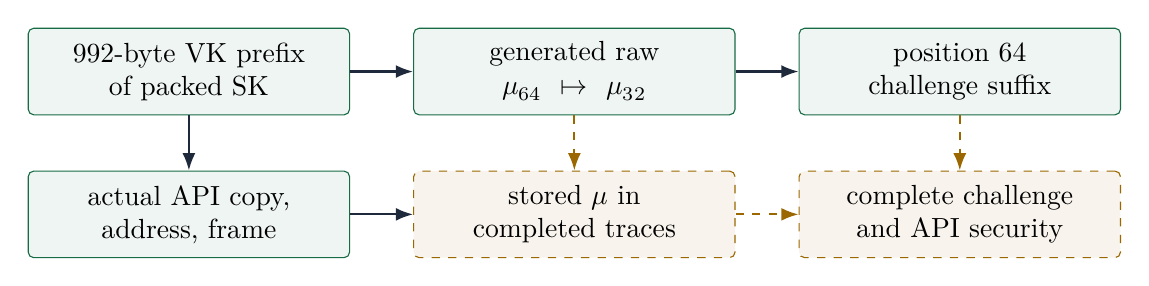
\begin{tikzpicture}[node distance=7mm and 8mm]
  \node[provennode] (kp) {992-byte VK prefix\\of packed SK};
  \node[provennode, right=of kp] (mu) {generated raw\\\(\mu_{64}\mapsto\mu_{32}\)};
  \node[provennode, right=of mu] (chal) {position 64\\challenge suffix};
  \node[provennode, below=of kp] (api) {actual API copy,\\address, frame};
  \node[partialnode, below=of mu] (trace) {stored \(\mu\) in\\completed traces};
  \node[partialnode, below=of chal] (top) {complete challenge\\and API security};
  \draw[flowarrow] (kp) -- (mu);
  \draw[flowarrow] (mu) -- (chal);
  \draw[flowarrow] (kp) -- (api);
  \draw[flowarrow] (api) -- (trace);
  \draw[openarrow] (mu) -- (trace);
  \draw[openarrow] (trace) -- (top);
  \draw[openarrow] (chal) -- (top);
\end{tikzpicture}
\caption{The key/transcript line. Solid arrows denote completed theorems;
dashed arrows denote open lifts.}
\label{fig:key-transcript-spine}
\end{figure}

\begin{figure}[ht]
\centering
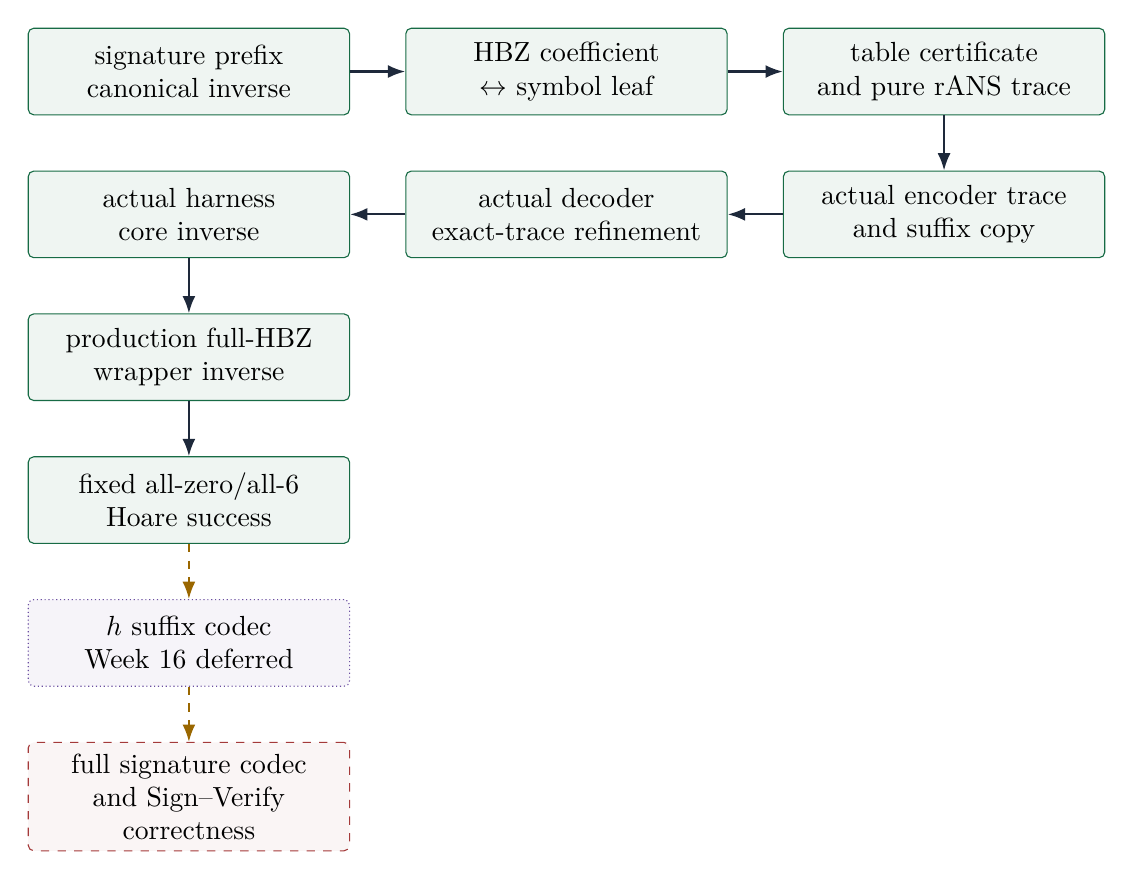
\begin{tikzpicture}[node distance=7mm and 7mm]
  \node[provennode] (prefix) {signature prefix\\canonical inverse};
  \node[provennode, right=of prefix] (leaf) {HBZ coefficient\\\(\leftrightarrow\) symbol leaf};
  \node[provennode, right=of leaf] (pure) {table certificate\\and pure rANS trace};
  \node[provennode, below=of pure] (copy) {actual encoder trace\\and suffix copy};
  \node[provennode, left=of copy] (loops) {actual decoder\\exact-trace refinement};
  \node[provennode, left=of loops] (core) {actual harness\\core inverse};
  \node[provennode, below=of core] (hbz) {production full-HBZ\\wrapper inverse};
  \node[provennode, below=of hbz] (witness) {fixed all-zero/all-6\\Hoare success};
  \node[deferrednode, below=of witness] (hcodec) {\(h\) suffix codec\\Week~16 deferred};
  \node[blockednode, below=of hcodec] (full) {full signature codec\\and Sign--Verify correctness};
  \draw[flowarrow] (prefix) -- (leaf);
  \draw[flowarrow] (leaf) -- (pure);
  \draw[flowarrow] (pure) -- (copy);
  \draw[flowarrow] (copy) -- (loops);
  \draw[flowarrow] (loops) -- (core);
  \draw[flowarrow] (core) -- (hbz);
  \draw[flowarrow] (hbz) -- (witness);
  \draw[openarrow] (witness) -- (hcodec);
  \draw[openarrow] (hcodec) -- (full);
\end{tikzpicture}
\caption{The signature-codec line. Week~11 closed the actual encoder's
successful suffix, Week~12 the actual decoder consuming an exact trace,
Week~13 core composition with actual copying in between, Week~14 the production
full-HBZ wrapper boundary, and Week~15 fixed all-6 failure exclusion.
The \(h\) codec was frozen when Week~16 switched to MINCORE.}
\label{fig:codec-spine}
\end{figure}

\subsection{Stage 1: the verification-key quotient of a packed secret key}

At the pure-array level, define
\[
  \operatorname{VKPrefix}_{992}(sk,vk)
  \Longleftrightarrow
  \forall,0\le i<992,\;sk_i=vk_i
\]
\sourcepath{PackedKeyPrefix.ec} proves these basic facts.

\begin{itemize}
  \item The byte-by-byte copy loop invariant is preserved at the next index;
  \item Copying all 992 bytes establishes the prefix relation;
  \item Writes from index 992 onward leave the completed prefix unchanged.
\end{itemize}

These array lemmas lift to the actual extracted procedure.

\begin{verified}[Prefix of the actual packer]
Under the mode~2 constants,
\theoremname{pack_sk_m23_mode2_vk_prefix} shows that when actual generated
\identifier{_pack_sk_m23} returns, the first 992 bytes of its secret-key array
equal the input verification-key array. The subsequent loops writing the
eta-vector and key preserve this prefix.
\end{verified}

\begin{verified}[Internal KeyGen return]
\theoremname{keypair_full_m23_mode2_return_prefix} and
\theoremname{keypair_internal_mode2_return_prefix} lift this relation to actual
generated KeyGen return values.
\[
  \text{KeyGen returns }(vk,sk)
  \Longrightarrow \operatorname{VKPrefix}_{992}(sk,vk).
\]
\end{verified}

Both are \statusproved\ partial-correctness theorems. They do not prove
termination of the KeyGen rejection loop, its complete output distribution,
or equivalence to the paper's KeyGen. Thus \claimid{FC-KG-TOP} remains
\statuspartial.

\subsection{Stage 2: from local arrays to public memory}

Using the array relation returned by KeyGen as actual API input to Sign/Verify
requires four kinds of arrow.

\begin{enumerate}
  \item Exporters copying local KeyGen VK/SK arrays to external addresses;
  \item The importer bringing external SK into Sign's local array;
  \item The importer bringing external VK into Verify's local array;
  \item A canonical bridge showing that integer and \(W64\) addresses
        describe the same regions.
\end{enumerate}

\sourcepath{ApiKeyMemoryBridge.ec} proves mode~2's 992/1408-byte prefixes and
disjoint frames for the actual copy helpers.

\begin{verified}[Sequential exports of actual raw KeyGen]
\theoremname{keypair_raw_api_exports_matching_prefixes} shows that when actual
\identifier{cryptolab_haetae_mode2_keypair_internal} returns, the first 992
bytes of the external SK and VK regions agree under explicit
valid/canonical/disjoint-region contracts.
\end{verified}

This is stronger than merely saying that a copy function copies, but weaker
than complete memory safety. Pointer validity and separation are explicit
premises, and KeyGen termination is still not a conclusion.

\subsection{Stage 3: generated raw \texorpdfstring{\(\mu\)}{mu} for Sign and Verify}

Sign absorbs the local packed-SK prefix and squeezes 64 bytes of \(\mu\).
Verify absorbs the VK region in global memory and squeezes 32 bytes.
The actual generated helper chain performs initialization, key/pre/message
absorption, Keccak permutation, finalization, and squeezing through different
procedure interfaces.

\sourcepath{ExtractedMuHashPrefix.ec} proves leaf relations, and
\sourcepath{ExactMuTopControl.ec} lifts them to the actual top procedures.

\begin{verified}[Generated raw \(\mu\) prefix]
Under explicit mode~2 key-prefix, equal pre/message-region, raw-branch,
and valid/no-wrap premises,
\[
  \mathsf{SignRawMu}\sim\mathsf{VerifyHashMu}
\]
holds with conclusion
\[
  \take_{32}(\mu^{64}_{\mathrm{Sign}})
  =\mu^{32}_{\mathrm{Verify}}
\]
The named theorem is
\theoremname{sign_verify_generated_raw_mu_prefix}.
\end{verified}

This theorem places the two actual generated procedures directly on its
theorem surface. It does not simply identify an abstract wrapper proposition
with actual procedures.
In addition, \theoremname{raw_prelen_shr63_zero} and
\theoremname{raw_prelen_branch_guard} show that the actual bit-level branch
selects the raw path.

\subsection{Stage 4: from whole-memory equality to read-region equality}

Once actual Sign has written a signature, there is no reason for the two
executions' entire global memories to agree. Only the key, pre, and message
regions read by the hash are needed.

\begin{verified}[Region-local generated hash]
\theoremname{sign_verify_generated_raw_mu_prefix_regionwise} allows different
global memories. When the key/pre/message read regions are related pointwise,
actual generated Sign/Verify raw-hash return values share the same 32-byte prefix.
\end{verified}

\begin{verified}[Sign output frame]
\theoremname{sign_raw_api_frames_reused_regions} shows that actual raw Sign
preserves VK/SK/pre/message regions disjoint from its outputs even while writing
1474 signature bytes and 8 siglen bytes.
\end{verified}

Together, these theorems establish the memory-level basis that the input bytes
Verify will read remain after Sign. The final transport directly comparing
stored \(\mu\) in two completed traces is still open, however.
That obligation is separated in \cref{sec:boundaries}.

\subsection{Stage 5: the position~64 challenge suffix}

Suppose Sign and Verify have the same challenge state and position, the
position is 64, and the preceding stage gives equal \(\mu_{32}\).
A theorem shows that running each actual generated absorb helper once leaves
equal states and positions.

\begin{verified}[Local challenge-suffix zero-loss]
\theoremname{generated_raw_mu_to_challenge_suffix_zero_loss} sequentially calls
the actual generated raw \(\mu\) procedure and actual generated 32-byte challenge
absorb helper on each side. Under the stated premises, the final
\((\mathit{state},\mathit{position})\) pairs agree.
\end{verified}

Deterministic loss is therefore zero at the raw/internal generated seam.
This theorem does not include the highbits/LSB prefix, complete challenge,
stored \(\mu\) in an actual accepted API trace, or the context branch.

\subsection{Stage 6: actual caller control and accepted Verify}

Weeks~4--6 placed these leaf results into actual public/raw caller contexts.
The following currently compile separately.

\begin{itemize}
  \item Exact \(\mu\) trace and hash-input binding for actual raw Sign;
  \item An exact trace preserving every early-reject/tail branch of actual raw/cryptolab Verify;
  \item The implication from Verify acceptance to reaching the actual tail and hash call;
  \item Binding showing that accepted Verify used actual VK/pre/message descriptors;
  \item An exact trace sequentially executing actual Sign and then actual Verify;
  \item A frame preserving key/pre/message regions during that sequential execution.
\end{itemize}

\begin{verified}[From acceptance to the tail]
For actual raw/cryptolab Verify,
\[
  \mathit{VerifyResult}=0
  \Longrightarrow \mathit{tail\_reached}
\]
is proved. This is neither the reverse implication nor a statement that an
arbitrary 1474-byte signature reaches the tail.
\end{verified}

\begin{verified}[Actual sequential trace]
\theoremname{raw_sign_then_verify_actual_exact_trace} matches return values and
final memory of actual raw Sign followed by actual raw Verify to sequential
execution of two instrumented traces.
\end{verified}

Nevertheless, \claimid{OBL-DIRECT-OBSERVED-MU} is \statuspartial.
An exact trace exposes observation locations and values, but does not
automatically transport a separate return-value pRHL theorem into equality
of ghost fields in two already completed traces.

\subsection{Stage 7: section--retraction for the actual signature prefix}

\sourcepath{Mode2SignaturePrefixPack.ec} and
\sourcepath{Mode2SignaturePrefixUnpack.ec} expose the exact layout of the
actual generated prefix loops.
\sourcepath{Mode2SignaturePrefixRoundTrip.ec} contains the harness calling
both procedures in their actual order.

\begin{verified}[Mode~2 prefix round trip]
For canonical challenge and canonical signed-low inputs,
\theoremname{pack_unpack_sig_prefix_mode2_roundtrip} establishes
\begin{align*}
  \mathit{decodedChallenge}[0..256)&=\mathit{challenge}[0..256),\\
  \mathit{decodedLow}[0..1024)&=\mathit{low}[0..1024)
\end{align*}
and frames the unused decoded-low tail.
\end{verified}

An all-zero witness for the canonical premises also compiles, so the
proposition is nonvacuous. The result nevertheless covers only the signature's
first 1056 bytes. It excludes the two metadata bytes, 416-byte suffix, padding,
and success of the complete unpacker.

\subsection{Stage 8: the HBZ coefficient--symbol leaf}

HBZ input comprises 1024 coefficients \(h_i\in[-6,7)\).
Prepare computes \(s_i=h_i+6\in\{0,\ldots,12\}\), and apply restores
\(s_i-6\) as a 32-bit word.

\begin{verified}[HBZ leaf inverse]
For a canonical HBZ array,
\theoremname{encode_prepare_decode_apply_mode2_inverse} shows that sequentially
executing actual prepare and actual apply restores the first 1024 coefficients,
preserves the decoder coefficient tail, and makes prepare's \(bad\) output zero.
\end{verified}

This is a leaf-level inverse bypassing the rANS core. It alone does not
establish a round trip for the actual compressed suffix.

\subsection{Stage 9: actual tables and pure rANS mathematics}

Mode~2 HBZ's 13 frequencies sum to 1024, and their cumulative intervals
partition \([0,1024)\).
\sourcepath{Mode2HbzTableCertificate.ec} proves this arithmetic as well as
the meaning of reciprocal/bias values and packed decoder words.
Separate files compile theorems that the actual generated literal arrays
satisfy that certificate.

\begin{verified}[Pure single-step inverse]
For each symbol \(s\) and admissible state \(x\), using \(c_s,f_s\) from the
actual table gives
\[
  D_s(E_s(x))=x
\]
The reciprocal-based fast encoder step also equals mathematical \(E_s\)
in the stated normalized range.
\end{verified}

Week~9 defined pure \(xs/cuts/bytes\) traces including normalization bytes
between individual steps.

\begin{verified}[Pure byte stack]
For canonical symbol lists, the following compile.
\begin{itemize}
  \item Normalization emits only 0, 1, or 2 bytes at each step;
  \item Appending emitted segments in decoder order restores the original state;
  \item The 4-byte little-endian initial state is recovered after parsing;
  \item Every trace state stays in \([2^{23},2^{31})\);
  \item The trace's head symbol, reduced state, and normalization segment
        decode one step at a time.
\end{itemize}
\end{verified}

\begin{verified}[Actual copying and control harness]
\theoremname{copy_encoded_suffix_correct} proves pointwise slice copying and
the tail frame of actual \identifier{__copy_encoded_suffix}.
\theoremname{actual_rans_harness_branches_on_encoder_result} shows that the
actual encoder, copy, and decoder are called in that order; the decoder runs
exactly when the encoder's actual \(bad\) result is zero, receiving
\((count,size,m)=(1024,\mathit{size},13)\).
\end{verified}

The control theorem itself concludes neither decoder success nor symbol
equality, final state, or byte-consumption count. Week~12's separate decoder
theorem proves those semantics under the exact-trace input relation, but at
that stage had not yet composed them into the control harness.
Week~13's \theoremname{actual_rans_encode_copy_decode_inverse} adds those
semantic conclusions to the same harness.

\subsection{Stage 10: local semantics of the actual encoder}

Week~10 incorporated \WeekTenTargetCount\ rANS encoder targets into the authored
target manifest and freshly compiled them. Rather than immediately assert one
large theorem between pure traces and actual generated procedures, these
separate array/list correspondence, word arithmetic, inner normalization,
and final serialization \cite{week10-report,rans-encoder-invariant}.

\begin{verified}[Array, word, and serialization lemmas]
\theoremname{encode_trace_suffix_extension} transports the actual 1024-byte
symbol-array suffix to a pure trace recurrence extending it one symbol at a
time. \theoremname{actual_mode2_encoder_word_step_correct} shows that the actual
word expression using literal-table reciprocals, shifts, biases, and complements
equals the pure fast step.
\theoremname{actual_encoder_final_state_serialization} shows that four
\identifier{set8} operations equal little-endian serialization of the 32-bit state.
\end{verified}

\begin{verified}[Actual inner loop and successful-output size]
\theoremname{actual_rans_encode_inner_no_underflow} installs byte-segment and
prefix-frame invariants in the nested normalization loop of actual generated
\identifier{_rans_encode}, establishing no underflow of the \(W64\) cursor.
\theoremname{actual_rans_encode_success_size_bound} is an actual
partial-correctness theorem: if that procedure returns, then
\[
  bad\ne0\quad\lor\quad
  \bigl(bad=0\land 0\le off\le1020\land
        4\le1024-off\le1024\bigr)
\]
\end{verified}

At the end of Week~10, this was stronger than the earlier
\(bad\in\{0,1\}\) control theorem, but did not state that the entire suffix
returned by the actual procedure equaled
\(
\operatorname{TraceBytes}
  (\operatorname{SymbolList}(symbols_0))
\).
The inner phase then used a conservative \(0..4\) range.
Procedure-level composition of the actual outer iteration's one-symbol state
transition and final four stores remained open.

\subsection{Stage 11: global trace closure of the actual encoder}

Week~11 added \WeekElevenTargetCount\ encoder targets, composing Week~10's
local transitions into the entire successful output
\cite{week11-report,rans-encoder-invariant}.
The central invariant remembers both the initial array \(enc_0\) and the
already processed pure suffix, rather than an arbitrary inner-loop entry array.

\begin{verified}[Tail-aware invariant and generated arithmetic]
The proposition \identifier{encoder_inner_tail_inv} states that the actual
inner loop preserves
\[
  \operatorname{InnerWrittenSuffix}(x_0,s,k)
  \mathbin{+\!\!+}\operatorname{EncodeTrace}(tail).bytes
\]
after the current cursor.

Lemma \theoremname{encoder_inner_tail_exit_exact} recovers
\(k=\operatorname{NormalizationLen}(x_0,s)\le2\) when the actual guard exits.
Lemma \theoremname{generated_loaded_nested_word_update} transports actual
table loads, reciprocal high products, shifts, complements, and biases
to the pure fast step.
\end{verified}

\begin{verified}[Encoder trace-closure theorem]
\theoremname{actual_rans_encode_trace_closure} directly opens actual generated
\identifier{RansEncodeTarget.M._rans_encode}. If it returns, it either fails
or, on success, establishes all of
\[
\begin{gathered}
  bad'=0,\qquad 0\le off'\le1020,\qquad
  4\le1024-off'\le1024,\\
  \operatorname{SegmentMatches}
    \bigl(enc',off',
      \operatorname{TraceBytes}(\operatorname{SymbolList}(symbols_0))\bigr),\\
  off'+\left|
    \operatorname{TraceBytes}(\operatorname{SymbolList}(symbols_0))
  \right|=1024,\qquad
  \operatorname{PrefixFrame}(enc_0,enc',off')
\end{gathered}
\]
\theoremname{actual_rans_encode_trace_refinement} is the corollary expanding
the same conclusion on the parent refinement surface.
\end{verified}

The theorem also composes the fact that the final four generated stores prepend
the serialized state to the accumulated normalization suffix.
Thus \claimid{OBL-RANS-ACTUAL-INNER-NORMALIZE},
\claimid{OBL-RANS-FINAL-SERIALIZATION}, and
\claimid{OBL-RANS-ENCODE-REFINEMENT} are each \statusproved\ within their stated
scopes. This remains Hoare partial correctness: it gives neither termination
of an actual call nor existence of an execution with \(bad'=0\).
The theorem alone therefore cannot establish success for a fixed input.
At Week~11, \claimid{OBL-RANS-ACTUAL-SUCCESS-WITNESS} was \statuspartial;
Week~15's separate all-6 theorem excludes failure in returning fixed-input
executions.

\subsection{Stage 12: exact-trace semantics of the actual decoder}

Week~12 added \WeekTwelveTargetCount\ decoder targets, installing pure-trace
coordinates into the actual generated decoder's two nested loops
\cite{week12-report,rans-decoder-invariant}.
The central input predicate \identifier{actual_mode2_decoder_trace_input}
does not accept an arbitrary buffer; it jointly requires the following.

\begin{itemize}
  \item The expected symbol array is a canonical mode~2 symbol stream;
  \item \(encoded\_size=|\operatorname{TraceBytes}
        (\operatorname{SymbolList}(expected))|\) and \(4\le encoded\_size\le1024\);
  \item \(buffer_0[0..encoded\_size)\) agrees pointwise with that exact trace;
  \item Each generated normalization read obtains the corresponding byte of
        the pure trace segment;
  \item Actual state fields are \((count,size,m)=(1024,encoded\_size,13)\);
  \item The actual mode~2 \identifier{symbol_words} and
        \identifier{dsyms_words} are used.
\end{itemize}

\begin{verified}[Decoder trace coordinates and invariant]
\identifier{decoder_state_at}, \identifier{decoder_cursor}, and
\identifier{decoder_segment_at} turn the pure \(xs/cuts/bytes\) trace's state,
cursor, and normalization segment into per-iteration coordinates.
The proposition \identifier{decoder_outer_trace_live} jointly preserves
\[
  x=\operatorname{DecoderStateAt}(i),\qquad
  off=\operatorname{DecoderCursor}(i)
\]
with equality of the decoded prefix and an untouched-tail frame.
The inner invariant replays exactly 0/1/2 bytes of the corresponding segment,
restoring the next pure state.
\end{verified}

\begin{verified}[Actual decoder exact-trace theorem]
\theoremname{actual_rans_decode_trace_refinement} directly opens actual generated
\identifier{RansDecodeTarget.M._rans_decode} and shows, if it returns,
\[
\begin{gathered}
  bad'=0,\qquad off'=encoded\_size,\\
  \forall i,\;0\le i<1024\Longrightarrow decoded'_i=expected_i,\\
  \forall i,\;1024\le i<2048\Longrightarrow decoded'_i=decoded_{0,i}
\end{gathered}
\]
It also derives the internal exit state \(x=2^{23}\), passing the actual final
reject test. Because the generated ABI does not return \(x\), however, only
returned arrays and state fields are exposed in the postcondition.
\end{verified}

Thus \claimid{OBL-RANS-DEC-NORMALIZE} and
\claimid{OBL-RANS-DECODE-REFINEMENT} are \statusproved\ as exact-trace Hoare
partial correctness.
At the end of Week~12, no sequential-harness theorem transported the encoder's
\identifier{segment_matches} and actual copying's \identifier{slice_eq}
into this input predicate. The next Week~13 stage closes precisely that edge.

\subsection{Stage 13: the actual encoder--copy--decoder core inverse}

Week~13 added \WeekThirteenTargetCount\ targets and composed the three calls
of actual \identifier{Mode2RansActualHarness.run} in order
\cite{week13-report,rans-core-composition}.
The harness and control theorem are in \sourcepath{Mode2RansActualInverse.ec};
semantic closure is separated into
\sourcepath{Mode2RansCoreCompositionBridge.ec} and
\sourcepath{Mode2RansCoreActualInverse.ec}.
The new bridge provides these transport lemmas.

\begin{itemize}
  \item \theoremname{copied_suffix_is_exact_trace}: obtains an exact trace at
        offset~0 of the copied buffer from encoder
        \identifier{segment_matches} and actual-copy \identifier{slice_eq};
  \item \theoremname{trace_bytes_trace_segment_nth}: decomposes global
        \identifier{trace_bytes} coordinates into per-symbol local-segment
        and decoder-cursor coordinates;
  \item \theoremname{segment_matches_implies_exact_decoder_segment_input}:
        obtains every pointwise decoder-byte-read premise from the global trace
        segment; \theoremname{segment_matches_implies_decoder_word_reads}
        transports these into actual W64 reads;
  \item \theoremname{actual_decoder_input_from_copied_trace} and
        \theoremname{configured_decoder_state_fields}: turn the copied trace
        and the three actual state stores, respectively, into components of the
        decoder input relation;
  \item \theoremname{actual_decoder_input_from_configured_trace}: constructs
        the entire Week~12 decoder input predicate from the copied trace,
        canonical symbol stream, size bound, and three actual state stores;
  \item \theoremname{encoder_success_size_word_bridge}: identifies actual
        (W64) subtraction with integer trace size in the no-wrap range.
\end{itemize}

\begin{verified}[\claimid{OBL-RANS-CORE-INVERSE}]
The semantic preconditions of
\theoremname{actual_rans_encode_copy_decode_inverse} are only harness-argument
binding and \identifier{mode2_hbz_symbol_stream}.
It does not assume encoder success, copied-trace equality, decoder execution,
or decoder success. If it returns, one of two branches holds:
\[
\begin{aligned}
\mathsf{failure}:\quad
  &encoderBad\ne0,\quad \neg decoderRan,\quad decoderOff=0,\quad decoderBad=1,\\
  &decoded'=decoded_0,\quad decoderState'=decoderState_0;\\[0.3em]
\mathsf{success}:\quad
  &encoderBad=0,\quad decoderRan,\quad (count,size,m)=(1024,encodedSize,13),\\
  &decoderBad=0,\quad decoderOff=encodedSize,\\
  &decoded'[0..1024)=expected[0..1024),\\
  &decoded'[1024..2048)=decoded_0[1024..2048).
\end{aligned}
\]
The success branch also preserves the actual encoder-suffix relation and initial
prefix frame. The core inverse of the three actual generated procedures
therefore compiles as success-conditioned partial correctness.
\end{verified}

\theoremname{core_composition_preconditions_satisfiable} uses an all-zero
canonical symbol array to show only nonvacuity of the premises.
Because the conclusion is a failure/success disjunction, neither reachability
of the actual success branch nor encoder/decoder termination follows.
Thus \claimid{OBL-RANS-ACTUAL-SUCCESS-WITNESS} remained \statuspartial\
at Week~13. This conclusion did not automatically lift to production full-HBZ
wrappers; the separate lift was closed in Week~14 and fixed all-6 failure
exclusion in Week~15.

\subsection{Stage 14: the production full-HBZ wrapper boundary}

Week~14 added \WeekFourteenTargetCount\ targets connecting focused full-HBZ
procedures to the actual SignaturePack/Unpack extraction boundary
\cite{week14-report,hbz-full-wrapper-composition}.
The proof chain has four layers.

\begin{enumerate}
  \item \sourcepath{Mode2HbzInternalBoundaries.ec} exactly connects prepare,
        rANS encode/decode, and apply calls inside the focused full wrappers
        to existing actual-procedure theorems.
  \item \theoremname{actual_encode_hb_z1_full_mode2_trace} preserves the
        failure/success branches of the actual full encoder on canonical HBZ
        coefficients. On success it provides a prepared-symbol witness,
        exact trace size/segment, and suffix frame.
  \item \theoremname{actual_decode_hb_z1_full_mode2_inverse} shows that,
        given that exact trace and prepared-symbol relation, the actual full
        decoder returns \(bad=0\), the original 1024-coefficient prefix,
        and the coefficient-tail frame.
  \item \theoremname{actual_hbz_full_encode_decode_inverse_mode2} composes
        the focused encode/decode harness, and
        \theoremname{signature_pack_unpack_hbz_full_actual_exact} matches
        it exactly to the production SignaturePack/Unpack harness, including
        the result tuple and \identifier{decoder_ran}.
\end{enumerate}

\begin{verified}[\claimid{OBL-SIG-HBZ-ENCODE-DECODE}]
The only semantic preconditions of the Hoare corollary
\theoremname{signature_pack_unpack_hbz_full_inverse_mode2} are argument binding
and \identifier{canonical_hbz_mode2}. If execution returns, this disjunction
holds:
\[
\begin{aligned}
\mathsf{failure}:\quad
  &size=0,\quad \neg decoderRan,\quad encoded=out_0,\\
  &decoded=decoded_0,\quad bad=bad_0;\\[0.3em]
\mathsf{success}:\quad
  &size\ne0,\quad 4\le size\le1024,\quad decoderRan,\quad bad=0,\\
  &decoded[0..1024)=hbz_0[0..1024),\\
  &\operatorname{CoeffTailFrame}(decoded_0,decoded),\quad
    \operatorname{SuffixFrame}(out_0,encoded),
\end{aligned}
\]
and the success branch has a prepared-symbol witness with
\identifier{segment_matches} for its \identifier{mode2_trace_bytes}.
Production-wrapper composition is therefore \statusproved\ as
success-conditioned partial correctness.
\end{verified}

The theorem does not assume encoder success; it preserves the actual failure
branch. The Week~14 theorem itself, however, proves neither failure exclusion
for a returning execution on canonical all-zero HBZ entering the actual
encoder's nonzero-size branch, nor encoder/decoder termination.
The fact that prepare produces an all-6 symbol stream and the actual encoder's
success are distinct propositions.
The former is composed with Week~15's separate budget/failure-cause theorem;
termination remains separate.

\subsection{Stage 15: fixed all-6 actual-success postconditions}

Week~15 added \WeekFifteenTargetCount\ targets, closing
\claimid{OBL-RANS-ACTUAL-SUCCESS-WITNESS} as fixed-input Hoare partial
correctness \cite{week15-report,rans-actual-success-witness}.
The first target, \sourcepath{Mode2RansAllSixBudget.ec}, proves the following
pure/prepare chain.

\begin{itemize}
  \item \theoremname{zero_hbz_get32}, \theoremname{zero_hbz_canonical}, and
        \theoremname{actual_prepare_zero_hbz_all_six} establish \(bad=0\)
        and a 1024-element all-6 prefix in the actual prepare return;
  \item \theoremname{symbol6_normalization_len_le1} shows that each symbol~6
        step emits at most one normalization byte;
  \item \theoremname{all_six_first_four_no_normalization} and
        \theoremname{all_six_normalization_budget} combine zero-byte emission
        in the first four steps with a total upper bound of 1020 bytes;
  \item \theoremname{all_six_trace_fits_mode2} adds the final four state bytes,
        placing total trace size in \([4,1024]\).
\end{itemize}

The existing encoder closure is strengthened by
\theoremname{actual_rans_encode_failure_trace_cause}, which concludes that
nonzero \(bad\) implies a normalization trace exceeding 1020 bytes.
Contradiction with the all-6 bound gives the following actual postconditions.

\begin{verified}[\claimid{OBL-RANS-ACTUAL-SUCCESS-WITNESS}]
\theoremname{actual_rans_encode_all_six_success} establishes \(bad=0\),
\(0\le off\le1020\), \(4\le1024-off\le1024\), an exact trace segment,
and a prefix frame for every returning execution of actual
\identifier{_rans_encode}.
\theoremname{actual_encode_hb_z1_full_zero_success} and
\theoremname{signature_pack_hbz_zero_success_mode2} lift this to the
focused/production full encoder.
\theoremname{signature_pack_unpack_hbz_zero_success_mode2} concludes the
production zero round trip, \identifier{decoder_ran}, decoder \(bad=0\),
and coefficient/encoded-tail frames.
\end{verified}

This proof does not require success as a precondition, but remains partial
correctness in Hoare logic. It includes no assertion that an actual fixed-input
execution terminates or exists, no losslessness or probability-one success,
and no \identifier{phoare} theorem.
Both “fixed all-6 Hoare success is \statusproved” and “fixed-input termination
is unproved” must therefore be retained.

\subsection{Stage 16: the frozen actual KeyGen snapshot and KG--NTT stopping boundary}

Week~16 added \WeekSixteenTargetCount\ MINCORE targets: three for KeyGen,
one for Sign, and four for Verify
\cite{week16-mincore-plan,week16-kg-report,week16-kg-ntt-mul-report,
week16-sign-report,week16-verify-report}.
In the first pure file,
\sourcepath{Mode2KeygenSnapshot}%
\allowbreak\sourcepath{Algebra.ec},
\theoremname{snapshot_residue_exact_low_high},
\theoremname{raw_sum_raw_residue_congruent_mod_2q}, and
\theoremname{snapshot_expression_from_product_congruent_mod_2q}
prove low/high decomposition of canonical residues and the doubled congruence.

File \sourcepath{Mode2KeygenCoreEquation.ec} defines the transparent harness
\begin{quote}
\identifier{ActualM23MatrixFinalizeSnapshot.run}.
\end{quote}
It snapshots the return of actual
\identifier{_kp_m23_matrix(2,3)}, then calls actual
\identifier{_keypair_finalize_m23(512)}.

\begin{verified}[Actual snapshot/finalizer boundary]
\theoremname{actual_m23_matrix_finalize_snapshot} composes the matrix-output/NTT
representation, exact finalization, and tail frame.
The strongest theorem,
\theoremname{actual_m23_matrix_finalize_semantic_snapshot}, adds
\theoremname{finalize_semantic_output_low_high_decomposition}, HAETAE finalizer
semantics, and \theoremname{finalize_semantic_output_snapshot_mod2q_zero},
yielding a KG-2-like decomposition, adjusted \(s_2\), and a snapshot-only
zero congruence mod-\(2q\) at every active coefficient.
\end{verified}

The third target, \sourcepath{Mode2KeygenNttMulBridge.ec}, fixes only the
last sound rewrite in the existing NTT chain, without duplicating actual loops.
Under the transformed-secret representation,
\theoremname{output_row_from_mode2_ntt_words} proves that
\identifier{output_row} equals exactly
\[
  \operatorname{array256\_mont}
  \bigl(\operatorname{full\_invntt}
    (\operatorname{pointwise\_row\_words}(m,v,row))\bigr)
\]
\theoremname{output_row_repr_from_mode2_ntt_words} transports this equality
to the existing \identifier{wide_slice_repr_bound} contract.
\theoremname{actual_m23_matrix_snapshot_rows_explicit} reuses the strongest
snapshot theorem by consequence, reducing both active rows to that
full-invNTT/pointwise-word representation.
None of these theorems assumes a native \(R_q\) product, security-model product,
or the desired KeyGen equation.

\begin{openobligation}[Frozen \claimid{OBL-MINCORE-KEYGEN}: \identifier{STOP-KG-NTT}]
At the frozen-paper stage, the final NTT-word rewrite compiled, but the
odd-root orthogonality/full-NTT convolution theorem converting actual
pointwise/inverse-NTT representation to native \(R_q\) negacyclic multiplication
was missing, as was the adapter transporting \identifier{Rq.poly} to the
security model's integer-list product. The row product
\(\sum_j A_{\mathrm{gen},ij}s_{\mathrm{gen},j}\) was therefore unavailable.
Faithful KG-1, KG-3, complete KG-4, and the paper equation
\(A s=qj\pmod{2q}\) were not proved.
\end{openobligation}

The KG-NTT-MUL audit identified these two missing leaves and ended at
\identifier{STOP-KG-NTT}, not \identifier{GO-KG}.
KeyGen was frozen at the KG-2/finalization boundary.
Sampling, retries, packing, the public API, KeyGen termination, and security
lie outside the conclusions of this actual two-call snapshot theorem.
Sign was subsequently frozen at \identifier{STOP-SIGN-CHAL-MODE2}, and
Verify at \identifier{STOP-VERIFY-MATRIX-CRT}
\cite{week16-sign-report,week16-verify-report,paper-freeze-artifacts}.

\subsection{Stage 17: post-freeze NTT/Rq transport and the actual avec/qj boundary}

Post-freeze work closed the first algebraic gap above without expanding the
frozen 82-target manifest.
In \sourcepath{NTTFullSpectralAction.ec},
\theoremname{rq_mul_coeff_foldr_to_bigi} and
\theoremname{full_ntt_montgomery_spectral_action} connect the
implementation-style negacyclic coefficient sum to full-NTT spectral action.
\theoremname{full_ntt_montgomery_row_product} composes this into a row product
for arbitrary column counts; \sourcepath{NTTMode2RowSpecializations.ec}
provides pure specializations for KeyGen's three columns and Verify's four.
This Verify result is not a theorem about actual
\identifier{_polyvec_ntt}/\identifier{_polymat_pointwise_acc}/
\identifier{_polyvec_invntt} procedures and does not close frozen
\identifier{STOP-VERIFY-MATRIX-CRT}.

\theoremname{rq_poly_add_repr}, \theoremname{rq_poly_mul_repr}, and
\theoremname{rq_poly_dot3_repr} in \sourcepath{RqHAETAEBridge.ec}, together
with \theoremname{keygen_mode2_row_product},
\theoremname{mode2_row_product_haetae_dot}, and
\theoremname{actual_m23_matrix_snapshot_rows_row_product} in
\sourcepath{Mode2KeygenNttMulBridge.ec}, transport the native \(R_q\)
three-term row product to the HAETAE \identifier{poly_dot} representation
\cite{post-freeze-kg-rq-haetae-report}.

\begin{verified}[Deterministic boundary of actual avec and the paper's \(a,qj\)]
\sourcepath{KgActualAvecQjSemantics.ec} fixes mode~2 row nonces 515/516,
\([3+row,2]\) after the 32-byte seed, SHAKE128 domain/padding 31/128,
168-byte blocks, little-endian 16-bit parsing, and \(<64513\) rejection.
\theoremname{mode2_uniform_stream_paper_a_flat} interprets the two
256-coefficient rows of the terminating actual sampler as the paper's \(a\).
The paper's \(j=(1,0)^T\) is separated through
\theoremname{paper_qj_row0_coeff0},
\theoremname{paper_qj_row0_other}, and
\theoremname{paper_qj_remaining_row}.
\theoremname{checked_mode2_parent_m23_finalize_actual_avec_qj} combines
current actual-sampler, matrix-helper, and finalizer results into one Hoare
boundary. This is partial correctness of terminating executions, not a
distribution, uniformity, losslessness, or termination claim.
\end{verified}

\begin{verified}[Faithful augmented coefficient-product composition]
The latest unmanifested standalone file
\sourcepath{KgFaithfulAugmentedModel.ec} instantiates a width-6 carrier with
actual arrays through
\identifier{faithful_augmented_matrix_coeff},
\identifier{faithful_augmented_secret_coeff},
\identifier{actual_faithful_augmented_matrix}, and
\identifier{actual_faithful_augmented_secret}.
\identifier{faithful_middle_matrix_poly} and
\identifier{faithful_middle_secret_poly} reconstruct the carrier's middle
three columns as HAETAE polynomials, so there is no free generated-block
argument detached from the displayed matrix/secret.
It then composes
\theoremname{actual_snapshot_paper_qj_to_faithful_augmented},
\theoremname{generated_product_coeff_from_rq_repr},
\theoremname{faithful_augmented_As_qj_from_generated_repr},
\theoremname{rq_as_haetae_poly_repr},
\theoremname{faithful_generated_row_product_haetae_dot},
\theoremname{actual_faithful_augmented_productE},
\theoremname{faithful_augmented_product_qj_from_generated_dot}, and
\theoremname{mode2_m23_facts_generated_row_product}.
The strongest theorem,
\theoremname{checked_mode2_parent_m23_finalize_faithful_augmented_paper_as_qj},
proves congruence mod-\(2q\) between
\identifier{faithful_augmented_matrix_vector_product_coeff} and
\identifier{faithful_qj_coeff} at each active coefficient of the actual
checked sampler/matrix/finalizer parent.
The file passed standalone \identifier{-no-eco} fresh compilation.

The exact endpoint is a structured coefficient product specific to the actual
carrier. \identifier{actual_faithful_augmented_productE} closes the expansion
of the product taking only matrix and secret as inputs.
The middle 2-by-3 block is reconstructed from the specified columns and
computed with HAETAE \identifier{poly_dot}.
The verdict for this work is \FaithfulAugmentedVerdict.
These dedicated mod-\(2q\) block semantics are not a coefficient theorem for
the existing width-4, mod-\(q\) security \identifier{matrix_vec_mul}, nor do
they identify security-side synthetic ExpandVecA with the actual sampler.
\cite{post-freeze-kg-faithful-augmented-report}
\end{verified}

\begin{openobligation}[\CurrentGate: \claimid{OBL-KG-SECURITY-EXPANDVECA-SEMANTICS}]
The existing security-side \identifier{haetae_mode23_qj_vector} is a
synthetic object using \identifier{public_key_seed_polyveck} tag 401.
\theoremname{security_named_qj_is_not_paper_qj} proves that its row~0
coefficient~0 is 401, whereas the paper's \(qj\) has \(q=64513\).
The zero-seed execution also has actual nonce-515 first coefficient 44985.
The security specification must therefore be replaced or refined with actual
SHAKE128/LE16/rejection/nonce semantics, keeping the paper's \(qj\) as a
separate correction, and an actual-array representation theorem must then
be proved. The paper-shaped congruence for the new custom carrier cannot
therefore be promoted to KG-1--KG-4 of the existing security model or
security-level \(A s=qj\pmod{2q}\)
\cite{post-freeze-kg-actual-avec-qj-report}.
\end{openobligation}

\subsection{Exact endpoints of the completed chains}

\begin{longtable}{@{}L{100mm} L{55mm}@{}}
\toprule
Chain & Endpoint \\
\midrule
\endfirsthead
\toprule
Chain & Endpoint \\
\midrule
\endhead
packed key \(\to\) generated raw \(\mu\) \(\to\) position-64 absorb &
\statusproved\ (raw/internal, local) \\
actual KeyGen export, Sign/Verify import, address/frame/control &
\statusproved\ (each named contract) \\
direct equality of stored \(\mu\) in completed actual traces &
\statuspartial \\
canonical signature prefix round trip &
\statusproved\ (1056-byte prefix) \\
HBZ leaf, table, pure rANS step and byte trace &
\statusproved\ (pure/leaf) \\
actual encoder array/list, word, and serialization leaves &
\statusproved\ (Week~10 local propositions) \\
actual encoder inner byte/frame and successful-output size &
\statusproved\ (exact \(0..2\), actual partial correctness) \\
actual encoder entire trace-suffix refinement &
\statusproved\ (success-conditioned partial correctness) \\
actual decoder exact-trace refinement &
\statusproved\ (1024-symbol recovery, exact consumption, tail frame) \\
actual encoder--copy--decoder harness control &
\statusproved\ (calls/branches only) \\
actual encoder--copy--decoder inverse &
\statusproved\ (success-conditioned partial correctness) \\
production full-HBZ wrapper inverse &
\statusproved\ (success-conditioned partial correctness, production boundary) \\
actual encoder success witness &
\statusproved\ (Hoare failure exclusion for fixed all-6 input;
no termination/losslessness) \\
actual KeyGen matrix/finalize snapshot &
\statuspartial\ (KG-2-like decomposition and snapshot congruence proved;
frozen paper ends at \identifier{STOP-KG-NTT} after the final NTT-word rewrite) \\
post-freeze full-NTT/native \(R_q\)/HAETAE row-product transport &
\statusproved\ (named pure/representation theorems outside the frozen 82 targets) \\
post-freeze actual \identifier{avec} and paper \(a,qj\) boundary &
\statuspartial\ (deterministic semantics and separate \(qj\) composition proved;
\CurrentGate\ at the security-object mismatch) \\
faithful augmented coefficient-product/transport &
\statusproved\ (standalone, outside the frozen 82 targets;
actual-carrier-specific product, not generic security-model
\identifier{matrix_vec_mul} equivalence) \\
actual accepted Sign core &
\statuspartial\ (call/branch control only; \identifier{STOP-SIGN-CHAL-MODE2}) \\
actual Verify core &
\statuspartial\ (helper-local word/control only; frozen \FrozenPaperGate) \\
\(h\) suffix codec &
\statusdeferred\ (Week~16 MINCORE KeyGen scope) \\
full signature codec and Sign--Verify correctness &
\statusblocked \\
implementation-level functional correctness and security &
\statusspecified / \statuspartial \\
\bottomrule
\end{longtable}

\section{The HBZ/rANS dynamical system and fixed-input failure exclusion}
\label{sec:rans-frontier}

\subsection{Why success postconditions and termination are different claims}

The inverse function for the signature prefix, the HBZ coefficient--symbol leaf,
the edge mapping canonical symbol streams through the actual encoder to pure byte
traces, the edge mapping exact traces through the actual decoder back to canonical
symbol streams, core composition across an actual copy, and the full-HBZ wrapper
boundary of production SignaturePack/Unpack have each been closed.
Week~15 excluded failure of the actual encoder when it returns on the all-6
stream produced by canonical all-zero HBZ, and lifted this to a production zero
round trip \cite{week15-report,rans-actual-success-witness}. Thus
\claimid{OBL-RANS-ACTUAL-SUCCESS-WITNESS} is \statusproved\ as fixed-input Hoare
partial correctness. It is not a termination/losslessness theorem guaranteeing
a return or the existence of an execution. After this result, the project moved
through the frozen Week~16 KeyGen/Sign/Verify \FrozenPaperGate\ to the
\CurrentGate\ of the post-freeze KeyGen semantics audit.

The integer arithmetic of rANS itself is not complicated. The difficulty lies
in implementation direction: the encoder reads symbols backwards and decrements
the byte-buffer cursor, while the decoder reads the copied buffer forwards.
The key is an invariant connecting the pure inverse-function theorem to the
states of the two actual nested loops. Week~11 completed the reverse-encoder
connection, Week~12 the forward-decoder connection, and Week~13 the actual copy
and premise transport between the two theorems. Week~14 composed this core
theorem with the prepare/apply, frame and size semantics of production
\identifier{_encode_hb_z1_full}/\identifier{_decode_hb_z1_full}.
Week~15 combines the fact that actual prepare produces an all-6 stream, a
1020-byte normalization budget, and a necessary condition for actual failure
to force the nonzero-size branch in returning fixed-input executions.
The remaining HBZ gaps are termination and existence of this execution itself,
global success on arbitrary canonical inputs, malformed rejection, and
probabilistic losslessness.

\subsection{The 13-symbol partition}

Mapping a canonical HBZ coefficient \(h_i\in[-6,7)\) to
\(s_i=h_i+6\) gives the alphabet
\[
  \Sigma=\{0,1,\ldots,12\}
\]
Let the rANS scale be \(M=1024\), and let each symbol's cumulative starting
point and frequency be
\[
\begin{aligned}
(c_s)_{s=0}^{12}
  &=(0,1,2,3,8,66,312,710,957,1016,1021,1022,1023),\\
(f_s)_{s=0}^{12}
  &=(1,1,1,5,58,246,398,247,59,5,1,1,1)
\end{aligned}
\]
The certificate establishes
\[
  f_s>0,\qquad \sum_{s=0}^{12}f_s=M,\qquad
  [c_s,c_s+f_s)\text{ partition }[0,M)\text{}
\]

This finite partition uniquely recovers the symbol from the residue slot
\(y\bmod M\). The fact that the actual encoder/decoder's packed tables represent
exactly these \(c_s,f_s\) values and the symbol lookup is also certified against
the generated literal arrays.

\subsection{The pure step is an inverse of Euclidean division}

For a fixed symbol \(s\), define
\begin{align*}
  E_s(x)
    &=\left\lfloor\frac{x}{f_s}\right\rfloor M
      +c_s+(x\bmod f_s),\\
  D_s(y)
    &=\left\lfloor\frac{y}{M}\right\rfloor f_s
      +(y\bmod M)-c_s
\end{align*}
Euclidean division
\(x=f_s\lfloor x/f_s\rfloor+(x\bmod f_s)\) and
\(0\le x\bmod f_s<f_s\) immediately suggest
\[
  D_s(E_s(x))=x
\]
The EasyCrypt theorems
\theoremname{pure_rans_step_quotient},
\theoremname{pure_rans_step_slot}, and
\theoremname{pure_rans_step_inverse} prove these calculations separately.

The actual encoder uses a fast formula with table reciprocals, shifts and biases
instead of division. A separate certificate shows that under
\[
  1\le x<x_{\max}(s),\qquad
  x_{\max}(s)=2^{21}f_s
\]
the fast quotient equals the Euclidean quotient, so \(D_s\) also inverts the
fast step. This is not merely a computational check that ``the table values look
right''; it is a theorem connecting the integer meanings of the actual word fields.

\begin{verified}[Pure and fast steps]
For canonical symbols \(0\le s<13\) and the specified state ranges,
\[
  D_s(E_s(x))=x,\qquad
  D_s(E^{\mathrm{fast}}_s(x))=x
\]
compile successfully. There is also a concrete witness to the premises at
\(s=0,x=1\), so the theorem is not vacuous.
\end{verified}

\subsection{Normalization bytes are coordinates of the discarded quotient}

When the state exceeds \(x_{\max}(s)\), divide it by the byte radix
\(B=256\) 0, 1 or 2 times to reduce it before applying the fast step.
The pure definitions are
\[
  \ell_s(x)\in\{0,1,2\},\qquad
  r_s(x)=\left\lfloor\frac{x}{B^{\ell_s(x)}}\right\rfloor
\]
and the low bytes discarded by division are retained in a list
\(\beta_s(x)\) in decoder read order.

The key readback proposition is
\[
  \operatorname{ReadBytes}(r_s(x),\beta_s(x))=x.
\]
For one byte, use \(x=B\lfloor x/B\rfloor+(x\bmod B)\); for two bytes, apply
this identity twice. The actual encoder writes the low byte first while
decrementing the cursor, so the final forward segment orders the two bytes as
\([\mathsf{high},\mathsf{low}]\). Missing this reversal can leave a pure theorem
correct while making it inconsistent with the actual decoder.

\sourcepath{Mode2RansNormalization.ec} provides leaf theorems showing that the
actual \(W32\) shift/truncate/or operations and \(W64\) cursor decrement have
the same meanings as these integer operations.

\subsection{A pure trace for the complete symbol list}

Let the symbol list be \(s_0,\ldots,s_{n-1}\), with \(n=1024\), and let the
final state be \(x_n=L=2^{23}\). Define recursively, so that the encoder proceeds
backwards,
\[
\begin{aligned}
  \ell_j&=\ell_{s_j}(x_{j+1}),\\
  r_j&=\left\lfloor x_{j+1}/256^{\ell_j}\right\rfloor,\\
  x_j&=E^{\mathrm{fast}}_{s_j}(r_j),\\
  \beta_j&=\beta_{s_j}(x_{j+1})
\end{aligned}
\]
The decoder-facing byte string is
\[
  \mathcal B=\operatorname{LE32}(x_0)
    \Vert\beta_0\Vert\cdots\Vert\beta_{n-1}
\]
Define the cursor cuts by
\[
  c_0=4,\qquad c_{j+1}=c_j+|\beta_j|
\]

The project names \(xs/cuts/bytes\) refer respectively to
\((x_0,\ldots,x_n)\), \((c_0,\ldots,c_n)\), and \(\mathcal B\).
These three objects are defined in \sourcepath{Mode2RansByteStack.ec}.
Its \identifier{valid_rans_trace} constructs them directly from the canonical
symbol list rather than assuming arbitrary witnesses.

\begin{verified}[Inductive inversion of the trace]
For a canonical list,
\[
  2^{23}\le x_j<2^{31}
\]
holds for every \(j\). Moreover, the residue slot of \(x_j\) selects \(s_j\),
\(D_{s_j}(x_j)=r_j\), and reading \(\beta_j\) recovers \(x_{j+1}\).
\end{verified}

The mathematics required for the pure decoder's list-level inductive proof is
therefore available. The refinement showing that actual encoder states represent
these trace coordinates was closed in Week~11; the refinement showing that actual
decoder states consume the same coordinates forwards was closed in Week~12.

\subsection{The six encoder targets audited in Week 10}

Week~10 decomposed the required outer-loop invariant into distinct transport
problems and added \WeekTenTargetCount\ files to the authored target manifest.
All six files compile freshly with \identifier{-no-eco}, but completion of each
local proposition must be distinguished from completion of the parent refinement.

\begin{itemize}
  \item \sourcepath{Mode2RansArrayListBridge.ec}: transports the actual byte
        array's symbol stream to a pure list and suffix, and expresses segment
        agreement and the prefix frame. The array--list bridge and one-symbol
        trace recurrence are \statusproved.
  \item \sourcepath{Mode2RansEncoderWordStep.ec}: connects actual word
        expressions using packed reciprocals, shifts and complements to the
        integer meaning of the pure fast step. Word-level equalities for the
        literal mode~2 table are \statusproved.
  \item \sourcepath{Mode2RansEncoderInnerProgress.ec}: represents the pure
        0/1/2-step progress of the normalization inner loop through the state,
        cursor and byte segment already written. This pure lemma is \statusproved.
  \item \sourcepath{Mode2RansEncoderSerialization.ec}: separates the four
        little-endian bytes of the final \(W32\) state, the exterior frame and
        successful size arithmetic. This leaf proposition is \statusproved.
  \item \sourcepath{Mode2RansEncoderTrace.ec}: supplies lemmas for finite
        phases, byte prepending, segments, prefix frames and absence of wrap
        used by the actual inner loop.
  \item \sourcepath{Mode2RansEncoderActualInner.ec}: installs these invariants
        in the actual generated \identifier{_rans_encode} inner loop and derives
        successful offset and size ranges through a separate actual Hoare theorem.
\end{itemize}

\begin{caution}[Local \statusproved\ and the then-\statuspartial\ parent in Week 10]
At the Week~10 baseline, these files certified only lemmas and local actual
partial correctness. Equality of the complete actual suffix with the pure
\identifier{trace_bytes} was absent, so
\claimid{OBL-RANS-ENCODE-REFINEMENT} was \statuspartial. The next section closes
exactly this parent edge in Week~11. These Week~10 targets did not certify success
branch reachability or termination. Fixed all-6 failure exclusion is a separate
Week~15 theorem, and termination remains open.
\end{caution}

\subsection{The actual encoder invariant closed in Week 11}

Let \(i\) be the actual reverse encoder's outer-loop index, \(x\) its current
word state, \(off\) the buffer cursor decreasing from the end, and \(enc\) the
buffer. With the pure trace
\[
  T_i=\operatorname{EncodeTrace}
       (\operatorname{SymbolSuffix}(symbols_0,i))=(x_i,b_i)
\]
the success branch's live invariant consists of the following five conditions
\cite{rans-encoder-invariant}.
\[
\begin{gathered}
  0\le i\le1024,\qquad x=x_i,\qquad off+|b_i|=1024,\\
  \operatorname{SegmentMatches}(enc,off,b_i),\qquad
  \operatorname{PrefixFrame}(enc_0,enc,off),\qquad 4\le off.
\end{gathered}
\]

Week~11 added \WeekElevenTargetCount\ targets. The tail-aware inner invariant
preserves the initial array \(enc_0\) and
\(\operatorname{EncodeTrace}(tail).bytes\) across actual byte writes and recovers
the exact \(0..2\) normalization length when the actual guard exits. Generated
word-step lemmas identify the word update after actual table loads and protect
erasure with the pure fast step; the final four generated stores prepend the
serialized state to the accumulated suffix.

Consequently, the actual procedure's success postcondition compiled as
\[
\begin{gathered}
  \operatorname{SegmentMatches}
  \bigl(enc',off',\operatorname{TraceBytes}
  (\operatorname{SymbolList}(symbols_0))\bigr),\\
  off'+\left|\operatorname{TraceBytes}
  (\operatorname{SymbolList}(symbols_0))\right|=1024,\\
  \operatorname{PrefixFrame}(enc_0,enc',off')
\end{gathered}
\]

\begin{verified}[\claimid{OBL-RANS-ENCODE-REFINEMENT}]
\theoremname{actual_rans_encode_trace_closure} shows that if the actual generated
\identifier{_rans_encode} returns, it either fails or, on success, satisfies all
three relations above, the offset/size ranges and \(bad=0\).
\theoremname{actual_rans_encode_trace_refinement} explicitly exposes equality of
the entire returned suffix at the parent refinement surface. Success is not a
premise; it is one branch of the conclusion determined by the actual return value.
\end{verified}

\begin{caution}[Limits of partial correctness]
This theorem alone does not establish actual encoder termination, success
reachability or an all-6 symbol success witness. In Week~11,
\claimid{OBL-RANS-ACTUAL-SUCCESS-WITNESS} was \statuspartial; the separate
Week~15 theorem excludes only failure in returning fixed all-6 executions.
\end{caution}

\subsection{The actual decoder invariant closed in Week 12}

For actual forward decoder index \(i\), state \(x\) and read cursor
\(off_d\), Week~12 installed the following invariant directly in the generated
outer/inner loops \cite{week12-report,rans-decoder-invariant}.

\begin{enumerate}
  \item The symbol prefix already output equals \(s_0,\ldots,s_{i-1}\);
  \item the current state is \(x_i\) and the current cursor is \(c_i\);
  \item table lookup selects \(s_i\) and reads the normalization segment
        exactly from \([c_i,c_{i+1})\);
  \item the frame of the unwritten tail of the output array is preserved;
  \item at exit, \(x=2^{23}\), \(off_d=size\), and \(bad=0\).
\end{enumerate}

The historical \theoremname{actual_rans_decode_mode2_control} fixed only the
actual tables/state fields and \(bad\in\{0,1\}\). The new input predicate
\identifier{actual_mode2_decoder_trace_input} combines the expected symbol
array, exact \identifier{trace_bytes}, pointwise relations for every
normalization read, state fields \((1024,encoded\_size,13)\), and actual
generated tables.

\begin{verified}[\claimid{OBL-RANS-DECODE-REFINEMENT}]
\theoremname{actual_rans_decode_trace_refinement} directly opens the actual
generated \identifier{_rans_decode} and, under this exact-trace input, recovers
all 1024 symbols and concludes \(off=encoded\_size\), \(bad=0\), and the decoded
tail frame. \theoremname{decoder_outer_trace_exit_components} internally derives
\(x=2^{23}\), also satisfying the actual final-state rejection check.
\end{verified}

This is Hoare partial correctness and does not establish decoder termination.
The exact-trace input is non-circular; Week~13 added a separate composition
theorem showing that the actual harness produces it.

\subsection{Actual harness core composition closed in Week 13}

The harness in \sourcepath{Mode2RansActualInverse.ec} is not an abstract assembly
diagram: it calls three actual generated procedures in the following order.
The theorem in that file closes only control of these calls; the Week~13
semantic closure is separate, in \sourcepath{Mode2RansCoreActualInverse.ec}.
\[
\mathsf{RansEncode}
\longrightarrow
\mathsf{CopyEncodedSuffix}
\longrightarrow
\mathsf{RansDecode}.
\]
The latter two calls run only when the encoder returns \(bad=0\).

The existing harness control conclusion is
\[
\begin{aligned}
  &\mathit{encoderBad}\in\{0,1\},\\
  &\mathit{decoderRan}\Longleftrightarrow\mathit{encoderBad}=0,\\
  &\mathit{decoderRan}\Longrightarrow
    (count,size,m)=(1024,\mathit{encodedSize},13)
\end{aligned}
\]
Week~13's \sourcepath{Mode2RansCoreCompositionBridge.ec} composes the encoder's
\identifier{segment_matches} and the copy's \identifier{slice_eq} into an exact
trace in the copied buffer, and transports it to the decoder's pointwise-read
and configured-state input predicate. In particular, it derives absence of wrap
from actual success bounds instead of silently replacing modular (W64)
subtraction with integer subtraction.

\begin{verified}[\claimid{OBL-RANS-CORE-INVERSE}]
\theoremname{actual_rans_encode_copy_decode_inverse} does not assume actual
encoder success. On failure, the actual copy and decoder are not run, and the
initial decoded array/state is preserved. On success, the following semantic
conclusions appear in the postcondition of the same harness theorem:
\[
  \mathit{decoderBad}=0,\quad
  off_{\mathrm{final}}=size,\quad
  decoded[0..1024)=symbols[0..1024).
\]
The decoder subproof also derives the internal exit state \(x=2^{23}\), but the
harness ABI does not expose it. The decoded tail \([1024,2048)\) is preserved
by a frame. This result is success-conditioned partial correctness.
\end{verified}

At the end of Week~13, no EasyCrypt theorem forced the actual success branch.
A concrete pure-trace witness, a canonical all-zero precondition witness, or a
size-4 decoder-state witness did not replace the postcondition that the actual
encoder returns \(bad=0\) on the concrete all-6 input. Week~15 closes exactly
this gap by contradicting the budget with the actual failure cause.

\subsection{Correctly reading the full HBZ wrapper closed in Week 14}

Because the actual encoder can express failure, canonical \(h\) alone must not
be used to assert an unconditional round trip. The parent proposition proved
in Week~14 must expose the failure branch, as in
\[
  size=0\quad\lor\quad
  \bigl(size\ne0\land bad=0\land
        decoded[0..1024)=h[0..1024)\bigr)
\]
Nonzero size bounds and buffer frames are also required.

\begin{verified}[\claimid{OBL-SIG-HBZ-ENCODE-DECODE}]
\theoremname{actual_hbz_full_encode_decode_inverse_mode2} proves this
failure/success disjunction for the focused actual full-HBZ harness.
\theoremname{signature_pack_unpack_hbz_full_actual_exact} shows that the
production SignaturePack/Unpack harness agrees exactly with the focused
harness in its return tuple and \identifier{decoder_ran} flag, and
\theoremname{signature_pack_unpack_hbz_full_inverse_mode2} lifts the same
contract to the production boundary. The success branch includes
\(4\le size\le1024\), coefficient-prefix recovery, coefficient/suffix frames,
and a prepared-symbol trace witness.
\end{verified}

\subsection{Week 15's fixed all-6 budget and actual failure exclusion}

Opening byte projections to prove that all actual 32-bit loads from
\identifier{zero_hbz} are 0 shows that actual prepare returns \(bad=0\) and a
prefix of 1024 symbol~6 entries. In the literal table, \(f_6=398\) and
\(x_{\max}(6)=2^{21}\cdot398\);
\theoremname{symbol6_normalization_len_le1} shows that each symbol~6 step with
\(2^{23}\le x<2^{31}\) emits at most one normalization byte.

The first four states computed from the initial state are
\[
  8388608\to21582496\to55528910\to142868116\to367580518
\]
and all four steps emit 0 bytes. Thus, even allowing one byte for each of the
remaining 1020 steps gives normalization length at most 1020; adding the final
four state bytes puts the total trace in \([4,1024]\). This is a conservative
capacity argument, not a claim that the observed exact 174/178-byte execution
has been proved as a theorem.

\begin{verified}[\claimid{OBL-RANS-ACTUAL-SUCCESS-WITNESS}]
\theoremname{actual_rans_encode_failure_trace_cause} states that a nonzero
\(bad\) from the actual encoder implies trace length \(>1020\). Contradicting
this with the all-6 upper bound lets
\theoremname{actual_rans_encode_all_six_success} establish \(bad=0\) and the
size/frame/exact-trace postconditions for every returning actual core execution.
\theoremname{actual_encode_hb_z1_full_zero_success},
\theoremname{signature_pack_hbz_zero_success_mode2}, and
\theoremname{signature_pack_unpack_hbz_zero_success_mode2} lift this conclusion
to the focused full wrapper including actual prepare and to the production
SignaturePack/Unpack zero round trip.
\end{verified}

\begin{caution}[\identifier{GO-WITNESS} is not \identifier{GO-WITNESS-LOSSLESS}]
These are Hoare partial-correctness theorems excluding failure in every
\emph{returning} fixed-input execution. Fixed-input termination, execution
existence (non-vacuity), losslessness, probability-one success and
\identifier{phoare} have not been proved. The \(h\) codec became
\statusdeferred\ because work moved to Week~16 MINCORE KeyGen, not because
the success witness was incomplete.
\end{caution}

\begin{center}
\begin{tabularx}{\textwidth}{Y L{31mm}}
\toprule
rANS layer & Status \\
\midrule
13-symbol intervals/frequencies and actual table certificate & \statusproved \\
pure quotient/slot/fast-step inverse & \statusproved \\
0/1/2-byte normalization and W32/W64 leaf semantics & \statusproved \\
canonical \(xs/cuts/bytes\) trace and state bounds & \statusproved \\
actual array/list suffix and word-step bridge & \statusproved \\
actual four-byte final serialization composition & \statusproved \\
actual encoder successful offset/size ranges & \statusproved\ (partial correctness) \\
actual inner normalization byte/frame/no-underflow &
\statusproved\ (tail-aware exact \(0..2\) exit) \\
actual encoded suffix copy and tail frame & \statusproved \\
actual encoder--copy--decoder branch control & \statusproved\ (control only) \\
actual encoder produces the complete pure trace &
\statusproved\ (success-conditioned partial correctness) \\
actual decoder consumes the exact trace &
\statusproved\ (1024-symbol recovery, exact consumption, tail frame) \\
actual encoder--copy--decoder core inverse &
\statusproved\ (success-conditioned partial correctness) \\
full HBZ encode/decode &
\statusproved\ (production-wrapper success-conditioned partial correctness) \\
actual encoder success witness &
\statusproved\ (fixed all-6 Hoare failure exclusion; no termination/losslessness) \\
\bottomrule
\end{tabularx}
\end{center}

\section{Open boundaries and limits on claims}
\label{sec:boundaries}

\subsection{The narrow but important semantic gap: product/replay}

The raw \(\mu\) line currently contains two separate facts.

\begin{enumerate}
  \item The \emph{return values} of the actual generated Sign/Verify hash calls
        have the same 32-byte prefix on related inputs;
  \item the actual complete Sign-then-Verify execution corresponds exactly to
        a ghost trace, which stores each hash result in \identifier{observed_mu}.
\end{enumerate}

The desired conclusion in an accepted Verify post-state is
\[
\begin{aligned}
  \mathit{VerifyResult}=0\Longrightarrow
  \operatorname{MuPrefix}_{32}(&
    \mathit{SignTrace.observed\_mu},\\[-0.3em]
    &\mathit{VerifyTrace.observed\_mu})
\end{aligned}
\]
Mathematically, combining facts 1 and 2 may appear immediate, but the variables
in the two propositions do not coexist at the same point in the current
program-logic surface.

\begin{center}
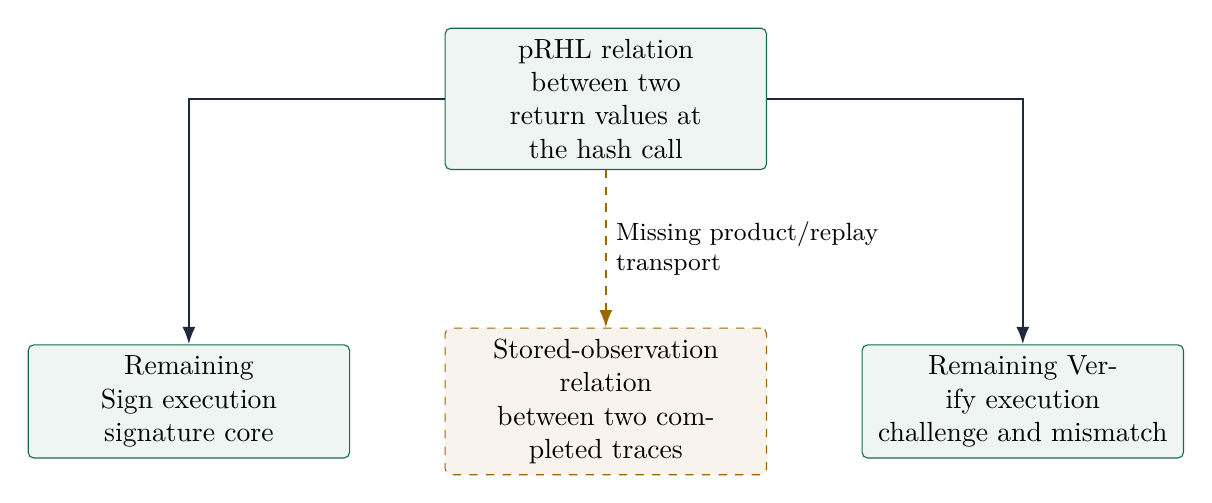
\begin{tikzpicture}[node distance=8mm]
  \node[provennode] (returns) {pRHL relation between two\\return values at the hash call};
  \node[partialnode, below=20mm of returns] (stored) {Stored-observation relation\\between two completed traces};
  \node[provennode, left=12mm of stored] (signcont) {Remaining Sign execution\\signature core};
  \node[provennode, right=12mm of stored] (verifycont) {Remaining Verify execution\\challenge and mismatch};
  \draw[openarrow] (returns) -- node[right,align=left,font=\small]{Missing product/replay\\transport} (stored);
  \draw[flowarrow] (returns.west) -| (signcont.north);
  \draw[flowarrow] (returns.east) -| (verifycont.north);
\end{tikzpicture}
\end{center}

The hash-call pRHL goal contains \(res\{1\},res\{2\}\), but those local return
variables disappear from the unary post-state after the entire trace completes.
Conversely, applying the pRHL theorem at the hash-call point requires handling
the different remaining continuations of Sign and Verify. Discarding the Sign
continuation on one side requires losslessness or an appropriate product rule,
neither of which is yet available.

\begin{openobligation}[\claimid{OBL-MU-PRODUCT-REPLAY}]
A sound rule or proof structure is needed to transport the return-value-level
region-local pRHL theorem to a stored-observation relation in an already
completed sequential trace.
\end{openobligation}

This obligation was frozen in Week~7 as \statusdeferred / an explicit paper
boundary \cite{product-replay}. The following approaches were deliberately rejected.

\begin{itemize}
  \item Assuming observation equality as a premise and restating the conclusion;
  \item adding a new SHAKE locality axiom;
  \item continually enlarging the theorem surface with another caller/observation wrapper;
  \item discarding the Sign continuation without a termination justification.
\end{itemize}

Accordingly, \(\delta_{\mu,\mathrm{raw\_api\_accept}}=0\) is not currently claimed.
This semantic gap arises from a missing program-logic transport arrow, not from
a lack of byte-locality theorems.

\subsection{Accepted-path and legitimate-signature correctness run in different directions}

The direction proved for actual Verify is
\[
  \operatorname{Accept}\Longrightarrow\operatorname{TailReached}
  \Longrightarrow\operatorname{HashInputsBound}
\]
This is a security-facing lane analyzing executions that have already accepted.

The direction required for functional correctness is
\[
  \sigma\leftarrow\operatorname{Sign}(sk,M)
  \Longrightarrow
  \operatorname{Verify}(vk,M,\sigma)=\operatorname{Accept}
\]
This requires showing that signatures produced by Sign pass every
unpacking, norm, hint, and challenge gates. A theorem in the first direction cannot be reversed
into one in the second direction.

\begin{openobligation}[\claimid{OBL-SIGN-OUTPUT-TAIL-REACH}]
Actual Sign output must be proved to pass actual Verify's early-reject tree and
reach the tail. The signature-prefix inverse and success-conditioned full-HBZ
wrapper are closed, and failure is also excluded for returning fixed all-zero
HBZ executions. However, this fixed input does not substitute for canonicality
of all actual Sign output. The \(h\) suffix, metadata/padding, norm, hint and
arithmetic correctness remain.
\end{openobligation}

\claimid{OBL-SIGN-VERIFY-CORRECTNESS} is \statusblocked\ by this obligation and
the remaining arithmetic and challenge correctness obligations.

\subsection{Representation obligations remaining in the full signature codec}

Extending the prefix's section--retraction to the full codec requires at least
the following squares. Week~14 closed one HBZ edge among them, and Week~15
excluded failure of returning fixed all-zero executions on that edge.

\begin{itemize}
  \item The two size-delta metadata bytes denote the same sizes in pack/unpack;
  \item the actual full HBZ rANS wrapper is an inverse under the success condition
        (\statusproved, Week~14);
  \item fixed-input Hoare success for canonical all-zero HBZ
        (\statusproved, Week~15; termination is unproved);
  \item encode/decode for the second, \(h\), suffix codec
        (\statusdeferred, transition to Week~16 MINCORE);
  \item canonicality of trailing zero padding and the parser's zero gate;
  \item preservation of array tails outside the target by the packer/unpacker;
  \item actual Sign produces canonical inputs and successful buffer bounds.
\end{itemize}

Thus \claimid{OBL-SIG-PREFIX-CODEC} is \statusproved\ in a limited sense, while
\claimid{OBL-SIG-FULL-CODEC-MODE2} is \statusblocked. The prefix inverse and full
inverse must not be described as the same proposition.

\subsection{Remaining algebraic, numerical and probabilistic obligations}

The frozen paper's MINCORE frontier was recorded as KeyGen
\identifier{STOP-KG-NTT}, Sign \identifier{STOP-SIGN-CHAL-MODE2}, and Verify
\FrozenPaperGate. Post-freeze work closed \identifier{rq_mul_coeff_foldr_to_bigi},
full-NTT spectral action, native \(R_q\) row products and HAETAE representation
transport, but a semantic mismatch between actual ExpandVecA and the existing
security-side synthetic object creates \CurrentGate. Separately, the actual
Verify 2-by-4 NTT/CRT/freeze procedure semantics remain a frozen obligation.
Full implementation refinement still requires the following independent obligations.

\begin{description}[leftmargin=39mm,style=nextline]
  \item[public-key algebra/NTT]
    \(R_q\)-module computations, NTT representations and the public-key relation
    agree with the actual implementation.
  \item[sampler distribution]
    The output distributions of uniform/small/hyperball samplers and the actual
    random tape agree with the paper distributions or have explicit distance bounds.
  \item[rejection and termination]
    KeyGen/Sign retries terminate, and the accepted distribution and retry loss
    are calculated.
  \item[highbits/LSB]
    Actual coefficient decomposition, rounding and packing agree with the paper's
    integer decomposition, and both challenge inputs are equal.
  \item[FIPS202 transcript]
    Every domain separator, length, absorb order and squeeze length agrees
    byte-for-byte with the fixed specification.
  \item[FFT tie policy]
    Fixed-point FFT, including boundary tie handling, is connected to the
    analytic predicate.
  \item[two-transcript extraction]
    The actual byte-level challenge and accepted signature instance are connected
    to two-transcript extraction in the paper/ROM reduction.
\end{description}

\subsection{The KG--NTT--MUL stopping boundary of frozen Week 16 KeyGen}

The transparent two-call harness for actual \identifier{_kp_m23_matrix} and
\identifier{_keypair_finalize_m23} places the pre-finalization \(bp\) snapshot,
finalizer semantics, KG-2-like low/high decomposition, adjusted \(s_2\), and a
snapshot-only mod-\(2q\) zero congruence in the same postcondition
\cite{week16-mincore-plan,week16-kg-report,week16-kg-ntt-mul-report}. This is
meaningful \statuspartial\ progress at the actual coefficient boundary of
\claimid{OBL-MINCORE-KEYGEN}.

The matrix helper's result is expressed as
\identifier{KeygenM23ArithmeticSpec.output_row}. The new
\theoremname{output_row_from_mode2_ntt_words} rewrites this exactly in terms of
actual full NTT, pointwise row products, inverse NTT and Montgomery representation;
\theoremname{actual_m23_matrix_snapshot_rows_explicit} applies that expression
to the transparent harness's two active rows.
At the frozen-paper point, there was neither a compiled theorem equating this
spectral expression with native \(R_q\) negacyclic multiplication nor an adapter
transporting \identifier{Rq.poly} into the security model's
\(A_{\mathrm{gen}}s_{\mathrm{gen}}\) representation. The KG-NTT-MUL audit
identified odd-root orthogonality/full-NTT convolution and this adapter as the
missing leaves and ended with \identifier{STOP-KG-NTT}. The frozen verdict
prohibits the following promotions.

\begin{itemize}
  \item Renaming snapshot \(\mathit{pre\_bp}\) to
        \(A_{\mathrm{gen}}s_{\mathrm{gen}}\) without justification;
  \item concluding faithful KG-1 or KG-3 from KG-2-like coefficient decomposition;
  \item concluding a complete KG-4 vector from one adjusted \(s_2\) component;
  \item promoting the snapshot congruence to the paper equation \(A s=qj\pmod{2q}\);
  \item inferring sampler, retry, packing, public API or KeyGen termination
        results from this two-call harness.
\end{itemize}

\subsection{Post-freeze KG progress and the new semantic boundary}

Post-freeze shared NTT theory proved pure coefficient normalization, full-NTT
spectral action and row products with arbitrary column counts. In Mode~2, pure
specializations for KeyGen's 3 columns and Verify's 4 columns both compile.
The KeyGen side was transported from native \(R_q\) row products to
\identifier{HAETAE_Algebra.poly_dot}
\cite{post-freeze-kg-rq-haetae-report}. However, the Verify 4-column theorem does
not open the actual helper loop and therefore does not clear \FrozenPaperGate.

The next audit connected actual \identifier{avec}'s SHAKE128 framing, nonces
515/516, little-endian candidates and \(<64513\) rejection to paper \(a\), and
independently added paper \(qj=q(1,0)^T\) to the snapshot zero equation.
However, the following three objects are distinct.

\begin{center}
actual SHAKE128/rejection \(a\)
\(\neq\) synthetic security generator,
\qquad paper \(qj\) is a separate correction.
\end{center}

A compiled counterexample shows that security-named row~0 coefficient~0 is 401,
whereas paper \(qj[0,0]=64513\). The actual value in the all-zero seed trace is
also 44985. Repairing \CurrentGate\ therefore requires replacing or refining
synthetic \identifier{public_rounding_vector_seed} with actual expansion semantics
and proving a coefficientwise actual-array representation
\cite{post-freeze-kg-actual-avec-qj-report}. Before crossing this boundary, the
following promotions are also prohibited.

\begin{itemize}
  \item Renaming the synthetic object to actual \identifier{avec} or paper \(qj\);
  \item assuming that the separate \(qj\) correction is preserved in a modulo-\(q\)
        HAETAE vector;
  \item renaming the new coefficient-product dedicated to the actual carrier
        as a security-level width-6 mod-\(2q\) equation without a theorem for
        general ring \identifier{matrix_vec_mul} defined solely from the existing
        security matrix/secret;
  \item inferring sampler distribution, uniformity, losslessness or termination
        from deterministic partial correctness.
\end{itemize}

\sourcepath{KgFaithfulAugmentedModel.ec} defines an actual width-6 carrier and
generated-product transport for this packaging and passes standalone fresh
compilation. \theoremname{actual_faithful_augmented_productE} expands the
dedicated structured coefficient-product as the sum of the head, generated
HAETAE \identifier{poly_dot}, and adjusted error.
\theoremname{checked_mode2_parent_m23_finalize_faithful_augmented_paper_as_qj}
proves coefficientwise congruence of this product with faithful \(qj\) for the
actual checked parent. The product takes only the actual matrix/secret as input;
the middle 2-by-3 block is \identifier{poly_dot} reconstructed from the specified
columns. The verdict for this work is therefore \FaithfulAugmentedVerdict.
However, this dedicated mod-\(2q\) evaluator is not the existing mod-\(q\)
security \identifier{matrix_vec_mul}, nor is it security-side ExpandVecA
equivalence. It therefore does not remove \CurrentGate.

\sourcepath{ImplementationSecurityGoals.ec} lists these items as
\identifier{obl_*} operations. Compiling the file means that the goal names and
composition interface are well-formed, not that each boolean has been proved true.

\subsection{Top-level functional correctness is still a specification}

\sourcepath{TopLevelGoals.ec} declares
\begin{align*}
  \mathsf{FC}_{\mathrm{KG}}
    &:\quad \mathsf{JKeyGen}_2=\mathsf{PaperKeyGen}_2,\\
  \mathsf{FC}_{\mathrm{Sign}}
    &:\quad \forall sk,M,
      \mathsf{JSign}_2(sk,M)=\mathsf{PaperSign}_2(sk,M),\\
  \mathsf{FC}_{\mathrm{Verify}}
    &:\quad \forall vk,M,\sigma,
      \mathsf{JVerify}_2(vk,M,\sigma)
      =\mathsf{PaperVerify}_2(vk,M,\sigma)
\end{align*}
as boolean specifications. For Sign/KeyGen, equality here includes equality
of probability distributions. The current prefix, memory, transcript and codec
theorems provide necessary deterministic subsquares, not the full equalities.

\subsection{The security composition formula is still a conditional interface}

The goal connecting implementation and paper scheme has the form
\[
  \Adv^{\mathrm{euf\mbox{-}cma}}_{\mathrm{Jasmin}}
  \le
  \Adv^{\mathrm{euf\mbox{-}cma}}_{\mathrm{paper}}
  +\delta_{\mathrm{KeyGen}}
  +q_{\mathrm{Sign}}\delta_{\mathrm{Sign}}
  +\delta_{\mathrm{Verify}}
  +\delta_{\mathrm{Encoding}}
\]
The current file declares loss variables and defines the inequality's interface,
but has not discharged every \(\delta\) and composed them into a final theorem.

The paper-level reduction interface further reduces to MLWE, BST-MSIS, ROM and
rejection/fork errors. \sourcepath{SecurityAssumptions.ec} restricts the
cryptographic interfaces that may remain in the final result to MLWE, BST-MSIS
and ROM. This does not mean that concrete game instances and a parameterized
reduction have been connected to the implementation's exact byte-level scheme.

\begin{caution}[Distinguishing declaration kinds]
Operations, assumptions and theorems are different. An operation declared without
a body, such as \identifier{op obl_sampler_distribution : bool.}, is an abstract
symbol expressing a goal. It is neither an axiom assuming the goal true nor a
theorem proving it true. The project's verification scripts separately prohibit
and scan for authored axioms and proof holes.
\end{caution}

\subsection{Trust boundary and out-of-scope items}

The current evidence chain trusts or fixes the following.

\begin{itemize}
  \item The 46-page HAETAE specification PDF with a recorded SHA-256 \cite{haetae-spec};
  \item the pinned \sourcepath{haetae-ref-jasmin/} implementation and focused
        extraction \cite{pinned-jasmin};
  \item the EasyCrypt kernel, Jasmin model, invoked SMT provers and build toolchain;
  \item source hashes and generated extraction/certificate manifests.
\end{itemize}

The conclusions of this sprint exclude the following.

\begin{itemize}
  \item Parameter sets other than mode~2;
  \item physical side channels, faults and RNG quality;
  \item claims that memory safety or constant-time automatically follow from EUF-CMA;
  \item end-to-end correctness of all actual hardware/compiler components;
  \item claims that full KeyGen, Sign, Verify or implementation EUF-CMA are complete.
\end{itemize}

\subsection{Current claim matrix}

\begin{longtable}{@{}L{47mm} L{27mm} L{70mm}@{}}
\toprule
Claim & Status & Exact boundary \\
\midrule
\endfirsthead
\toprule
Claim & Status & Exact boundary \\
\midrule
\endhead
VK prefix of packed SK & \statusproved &
First 992 bytes upon return from the actual generated packer/Internal KeyGen \\
raw \(\mu\) generated seam & \statusproved &
64-to-32 prefix on the raw branch and related key/pre/message regions \\
position-64 challenge suffix & \statusproved &
32-byte absorb from equal initial state/position \\
actual API key copy/address/frame & \statusproved &
Under each named valid/canonical/disjoint contract \\
accepted Verify tail/input binding & \statusproved &
Direction accept \(\Rightarrow\) tail/hash inputs \\
stored observed \(\mu\) equality & \statuspartial &
Missing product/replay transport \\
signature prefix inverse & \statusproved &
Canonical challenge/low, first 1056 bytes \\
HBZ leaf inverse & \statusproved &
First 1024 coefficients, excluding rANS \\
actual rANS table and pure step & \statusproved &
Concrete 13-symbol table, specified state range \\
pure normalization byte trace & \statusproved &
Canonical symbol list, not an actual loop \\
actual array/list and word-step bridge & \statusproved &
1024-symbol suffix recurrence, literal table word equalities \\
actual final serialization leaf & \statusproved &
Composition of four actual stores with little-endian serialization of the accumulated trace \\
actual encoder success size & \statusproved &
If it returns, failure or \(0\le off\le1020\), \(4\le1024-off\le1024\) \\
actual inner normalization & \statusproved &
Byte segment, frame, no-underflow and exact pure \(0..2\) exit \\
actual encoder trace refinement & \statusproved &
Complete suffix equality in success-conditioned partial correctness \\
actual decoder trace refinement & \statusproved &
Exact-trace partial correctness, 1024-symbol equality, exact byte consumption and tail frame \\
actual rANS harness control & \statusproved &
Only the actual call order and success/failure branches are complete \\
actual rANS core inverse & \statusproved &
Success-conditioned partial correctness of actual encoder/copy/decoder \\
actual encoder success witness & \statusproved &
Failure exclusion for returning fixed all-zero/all-6 executions; no termination/losslessness \\
production full-HBZ wrapper inverse & \statusproved &
Success-conditioned composition of prepare/apply, rANS core and production lift is complete \\
actual KeyGen matrix/finalize snapshot & \statuspartial &
KG-2-like decomposition and snapshot mod-\(2q\) identity proved;
in the frozen paper, \identifier{STOP-KG-NTT} after the final NTT-word rewrite \\
post-freeze NTT/Rq/HAETAE row products & \statusproved &
Pure spectral action, native \(R_q\) 3-column/4-column row products and KeyGen
3-column HAETAE representation transport; actual Verify procedure excluded \\
post-freeze actual \identifier{avec}/paper \(a,qj\) & \statuspartial &
Deterministic expansion and separate \(qj\) snapshot composition proved;
\CurrentGate\ at the synthetic security semantics mismatch \\
faithful augmented coefficient-product composition & \statusproved &
Standalone actual-carrier structured product \(\equiv qj\); outside the frozen
82-target set; generic security-model \identifier{matrix_vec_mul}/ExpandVecA equivalence excluded \\
actual Sign accepted core & \statuspartial &
Only call and accept-branch control for the three actual helpers;
\identifier{STOP-SIGN-CHAL-MODE2} \\
actual Verify core sequence & \statuspartial &
Actual five-helper sequence, V-1/V-2/V-5/V-6 word projections, local norm/tail results;
frozen \FrozenPaperGate \\
\(h\) suffix codec & \statusdeferred &
Scope moved to Week~16 MINCORE KeyGen; inverse not attempted \\
full signature codec & \statusblocked &
\(h\), metadata, padding and residual frames remain after the HBZ wrapper \\
Sign output tail reach & \statuspartial &
Only prefix and success-conditioned HBZ wrapper closed; \(h\), metadata/padding,
norm/hint/arithmetic remain \\
FC-KeyGen/Sign/Verify & \statusspecified / \statuspartial &
Only some deterministic lower-level seams proved, including the KeyGen snapshot \\
Implementation EUF-CMA & \statusspecified &
Loss and paper-reduction connections incomplete \\
\bottomrule
\end{longtable}

\section{Dependency-ordered next steps and contribution points}
\label{sec:roadmap}

\subsection{The current single priority: repairing security ExpandVecA semantics}

The latest post-freeze gate is \CurrentGate. The first obligation is
\begin{quote}
\CurrentPriority
\end{quote}
Post-freeze NTT/Rq/HAETAE transport and the interpretation of actual
\identifier{avec} as paper \(a\) have compiled. However, the existing security-side
object is a synthetic generator, neither the actual SHAKE128/rejection expansion
nor paper \(qj\). Composing the full KeyGen equation without repairing this mismatch
would equate the concrete coefficients 44985 and 401. Meanwhile, the frozen
paper's \FrozenPaperGate\ is a separate status. Although a pure 2-by-4 row-product
specialization became available post-freeze, the actual Verify helper loop and
CRT/freeze procedure theorems remain open.

\begin{figure}[ht]
\centering
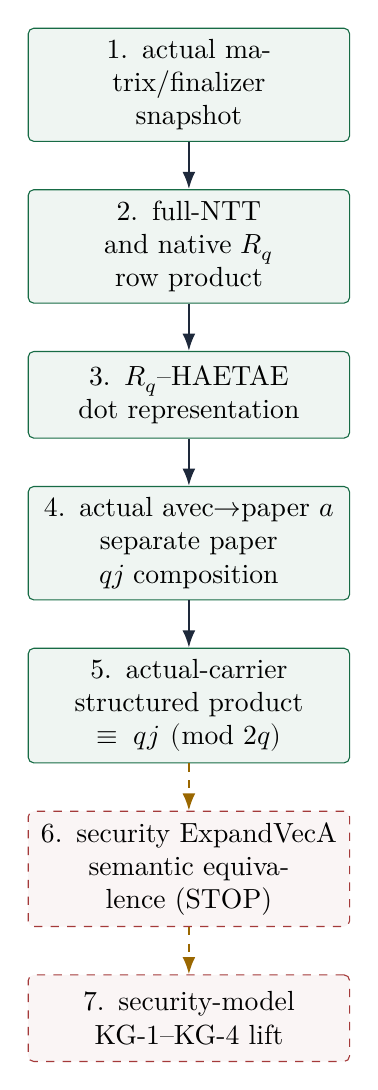
\begin{tikzpicture}[node distance=6mm]
  \node[provennode] (snapshot) {1. actual matrix/finalizer\\snapshot};
  \node[provennode, below=of snapshot] (ntt) {2. full-NTT and native \(R_q\)\\row product};
  \node[provennode, below=of ntt] (repr) {3. \(R_q\)--HAETAE\\dot representation};
  \node[provennode, below=of repr] (avec) {4. actual \identifier{avec}\(\to\)paper \(a\)\\separate paper \(qj\) composition};
  \node[provennode, below=of avec] (faithful) {5. actual-carrier structured product\\\(\equiv qj\pmod{2q}\)};
  \node[blockednode, below=of faithful] (security) {6. security ExpandVecA\\semantic equivalence (STOP)};
  \node[blockednode, below=of security] (paper) {7. security-model\\KG-1--KG-4 lift};
  \draw[flowarrow] (snapshot) -- (ntt);
  \draw[flowarrow] (ntt) -- (repr);
  \draw[flowarrow] (repr) -- (avec);
  \draw[flowarrow] (avec) -- (faithful);
  \draw[openarrow] (faithful) -- (security);
  \draw[openarrow] (security) -- (paper);
\end{tikzpicture}
\caption{The current post-freeze KeyGen cut. The coefficient-product dedicated to
actual carriers is closed, but work stopped at generic security
ExpandVecA/\identifier{matrix_vec_mul} semantics.}
\label{fig:next-order}
\end{figure}

On the codec line, Week~15 closed failure exclusion for returning fixed all-6
executions. Fixed-input termination/losslessness remain open, however, and the
\(h\) suffix codec became \statusdeferred\ when scope moved to this one-week
MINCORE effort. Both facts are independent of the current KeyGen blocker.

\subsection{Stage 1 complete: encoder}

\claimid{OBL-RANS-ENCODE-REFINEMENT} was closed by
\theoremname{actual_rans_encode_trace_closure}, which opens actual
\identifier{_rans_encode}, and its expanded corollary
\theoremname{actual_rans_encode_trace_refinement}. The success-branch
postcondition establishes all of the following together.

\begin{itemize}
  \item The actual output suffix equals the canonical symbol list's
        \identifier{trace_bytes} pointwise;
  \item at each outer iteration, the actual word state equals the suffix's pure
        \identifier{encode_trace} state;
  \item actual \(off\) and trace-byte length satisfy
        \(off+|\operatorname{TraceBytes}|=1024\);
  \item the already proved final 4-byte state serialization is composed before
        the normalization suffix, fixing segment order;
  \item the unwritten-prefix frame is preserved;
  \item the failure branch is not hidden.
\end{itemize}

Week~10's array/list suffix recurrence, actual reciprocal word step, inner
byte/frame/no-underflow results, final serialization leaf and successful
offset/size ranges were connected to Week~11's tail-aware outer/inner invariants,
generated table load--protect--word-update lemmas and final-store composition.
Consequently, the suffix of the actual returned buffer, rather than an arbitrary
valid trace or a fresh witness buffer, agrees with the canonical trace bytes.

This is nevertheless Hoare partial correctness. A success witness showing that
an actual execution reaches the success branch, and termination, do not follow
from this Week~11 theorem alone. Week~15 separately excluded failure in returning
fixed all-6 executions, but termination still remains.

\subsection{Stage 2 complete: decoder}

\claimid{OBL-RANS-DECODE-REFINEMENT} was closed by
\theoremname{actual_rans_decode_trace_refinement}, which opens actual
\identifier{_rans_decode}. Under the exact-trace input relation, induction proved
the following.

\begin{itemize}
  \item At iteration \(i\), the decoded prefix equals the original symbol prefix;
  \item state/cursor equal the pure \(x_i,c_i\);
  \item actual table lookup selects the interval partition's unique \(s_i\);
  \item the nested normalization loop consumes \(\beta_i\) in the exact order;
  \item \(state=2^{23}\) is derived at the internal loop exit, and the return
        values establish \(off=size\) and \(bad=0\);
  \item the decoded tail frame.
\end{itemize}

Connecting encoder and decoder directly in lockstep enlarges the proof surface
because of their reverse/forward directions and the intervening buffer copy.
The two refinements were verified independently using the already constructed
pure trace as a common intermediary. This decoder theorem assumes an input
trace and establishes Hoare partial correctness, not termination.

\subsection{Stage 3 complete: actual harness inverse}

\claimid{OBL-RANS-CORE-INVERSE} was closed by
\theoremname{actual_rans_encode_copy_decode_inverse} in
\sourcepath{Mode2RansCoreActualInverse.ec}. This theorem directly concerns the
actual harness defined in \sourcepath{Mode2RansActualInverse.ec} and derives the
following semantic conclusions. The two filenames refer respectively to
``harness definition/control'' and ``Week~13 semantic inverse''; the latter
was proved separately to prevent misreading the former's control-only theorem
as a semantic result.

\begin{itemize}
  \item The encoder failure branch remains explicit and does not run the decoder;
  \item \identifier{segment_matches} of the encoder's successful suffix is
        composed with \identifier{slice_eq} of the actual copy;
  \item the copied buffer supplies the decoder's pointwise exact-read premises;
  \item actual decoder return gives \(bad=0\), exact consumption, 1024-symbol
        equality and the tail frame;
  \item no arbitrary trace, fresh witness buffer or encoder success is added
        as an external premise.
\end{itemize}

This is success-conditioned partial correctness. The canonical all-zero array
shows non-vacuity of the premises but does not automatically establish existence
of encoder success or termination of the complete execution. In Week~13,
success reachability was a separate obligation,
\claimid{OBL-RANS-ACTUAL-SUCCESS-WITNESS}; Week~15 closed only its fixed all-6
Hoare postcondition.

\subsection{Stage 4 complete: production full-HBZ wrapper}

\claimid{OBL-SIG-HBZ-ENCODE-DECODE} was closed by
\theoremname{signature_pack_unpack_hbz_full_actual_exact} and
\theoremname{signature_pack_unpack_hbz_full_inverse_mode2}. The chain directly
opening actual \identifier{_encode_hb_z1_full} and
\identifier{_decode_hb_z1_full} concludes the following.

\begin{itemize}
  \item Actual prepare maps canonical HBZ coefficients to a canonical symbol stream;
  \item the actual rANS core theorem's failure/success branches are preserved;
  \item on success, actual apply maps recovered symbols back to the original
        coefficients;
  \item wrapper-level size, state and input/output tail frames are connected;
  \item no actual success witness or decoder result is required again as an
        external premise.
\end{itemize}

This stage is \statusproved\ as success-conditioned partial correctness
\cite{week14-report,hbz-full-wrapper-composition}. General reachability of the
actual success branch and termination are separate theorems. Week~15 excludes
failure only for returning executions on the fixed all-zero input.

\subsection{Stage 5 complete: fixed all-6 success postcondition}

Week~15's \theoremname{actual_rans_encode_all_six_success} derives \(bad=0\)
for returning fixed-input executions by contradicting the theorem that actual
failure requires trace length \(>1020\) with the all-6 trace budget \(\le1020\).
Focused/production lifts establish \(4\le size\le1024\), exact trace/frame
and the zero coefficient round trip together
\cite{week15-report,rans-actual-success-witness}.

The completion verdict at this stage is fixed-input Hoare partial correctness.
It is not promoted to termination, losslessness, non-vacuous execution or
\identifier{phoare}. The originally planned subsequent \(h\) suffix,
metadata/padding, full signature inverse and Sign output tail reach remain
respectively deferred or blocked after the transition to Week~16 MINCORE.

\subsection{Stage 6 frozen stop: KG--NTT--MUL audit}

\theoremname{output_row_from_mode2_ntt_words} and
\theoremname{actual_m23_matrix_snapshot_rows_explicit} closed the final sound
edge rewriting \identifier{KeygenM23ArithmeticSpec.output_row} into actual
full-invNTT/pointwise word expressions and applying them to two active rows
\cite{week16-kg-ntt-mul-report}. At the frozen-paper point, the following two
arrows were absent:
\[
  \operatorname{array256\_mont}
    (\operatorname{full\_invntt}(\widehat a\odot\operatorname{full\_ntt}(p)))
  \;\not\Longrightarrow\;
  (\operatorname{full\_invntt}\widehat a)\star_{R_q}p,
\]
and the adapter transporting native \identifier{Rq.poly} multiplication to the
security model's integer-list \identifier{poly_mul}/\identifier{matrix_vec_mul}
was also absent. The first arrow required odd-root orthogonality and full-NTT
convolution. The time-bounded audit did not assume them as new premises and
ended with \identifier{STOP-KG-NTT}. Post-freeze work closed these pure-algebra
and \(R_q\)--HAETAE representation gaps, but does not change this historical
frozen verdict itself.

\subsection{Stage 7 frozen: accepted Sign core}

Sequential execution of the following three actual helpers was composed in a
transparent harness and compiled through its control theorem.
\begin{center}
\identifier{_sf_round_challenge_mode2}\quad
\identifier{_sf_z_check}\quad
\identifier{_sf_hint_mode2}
\end{center}
The compiled control theorem in \sourcepath{Mode2SignAcceptedCore.ec} is
\begin{center}
\theoremname{actual_sign_accepted_core_branch_control_mode2}
\end{center}
However, the headline S-1--S-7 theorem was frozen at
\identifier{STOP-SIGN-CHAL-MODE2} because
\identifier{sf_challenge_mode2_highbits_lsb_sampleinball_correct} is absent.
For returning, accepted executions, commitment/challenge, the response
\(z=y+(-1)^bcs\), two exact integer norm predicates and the coefficientwise hint
equation must be derived \cite{week16-mincore-plan,claim-ledger}.

The headline theorem must not yet be counted as a compiled proof. Its
precondition must not assume \identifier{reject=0} or the final equations.
Sampler distributions, signing-loop termination, packing and the complete
1474-byte signature are outside this stage's scope.

\subsection{Stage 8 frozen stop: actual Verify helper chain}

In \sourcepath{Mode2VerifyCoreSequence.ec},
\theoremname{actual_verify_core_sequence_branch_control_mode2} and
\theoremname{actual_verify_core_sequence_input_snapshots_mode2} fix the actual
Verify five-helper call sequence and input snapshots.
\sourcepath{Mode2VerifyPrepareNorm.ec},
\sourcepath{Mode2VerifyRecover.ec}, and
\sourcepath{Mode2VerifyTailChallenge.ec} respectively provide
\theoremname{verify_prepare_z1_wprime_mode2_word_exact},
\theoremname{actual_sign_verify_recover_w_z2_mode2_word_semantics},
\theoremname{verify_tail_exact_trace_mode2}, and
\theoremname{poly_mismatch_mode2_word_exact}
\cite{week16-verify-report}. Thus V-1/V-2/V-5/V-6 projections, the W64 norm gate,
and tail trace/mismatch expression are closed at helper-local scope.

However, \identifier{verify_matrix_ntt_acc_mode2_cols4_correct} for actual 2-by-4
\identifier{_polyvec_ntt}/\identifier{_polymat_pointwise_acc}/
\identifier{_polyvec_invntt}, and
\identifier{verify_crt_freeze_mode2_word_exact} for actual from-CRT/freeze,
are absent. The challenge leaf
\identifier{verify_tail_m23_highbits_lsb_sampleinball_correct} also remains
independently open. This is the frozen \FrozenPaperGate. The post-freeze pure
\theoremname{verify_mode2_row_product_from_reprs} supplies the first procedure
leaf's algebraic goal but does not replace actual loop refinement.

\subsection{Stage 9 in progress: post-freeze actual avec/qj audit}

\theoremname{rq_mul_coeff_foldr_to_bigi}, full-NTT spectral action, generic row
products, native \(R_q\) 3-term products and HAETAE dot representation are
now \statusproved. The actual sampler side also interprets nonces 515/516,
SHAKE128 framing, little-endian parsing, \(<64513\) rejection and unchanged
storage as paper \(a\), and separately composes paper \(qj\) into the snapshot
equation \cite{post-freeze-kg-rq-haetae-report,
post-freeze-kg-actual-avec-qj-report}.

The first current goal is \claimid{OBL-KG-SECURITY-EXPANDVECA-SEMANTICS}.
The specification must be replaced/refined so that security
\identifier{public_rounding_vector_seed} has the same semantics as actual
expansion, and a coefficientwise actual-array representation must be proved.
The actual-carrier width-6 coefficient-product packaging that separately preserves
the paper \(qj\) correction is closed in the latest
\sourcepath{KgFaithfulAugmentedModel.ec}. Through actual matrix/secret
concretization, generated HAETAE \identifier{poly_dot} transport and
\theoremname{actual_faithful_augmented_productE}, this file composes the actual
checked parent's product equation \(\equiv qj\pmod{2q}\) as a standalone,
freshly compiled theorem. This product takes only the actual matrix/secret as
input and reconstructs the middle 2-by-3 block from its columns, giving the
verdict \FaithfulAugmentedVerdict. The remaining obligation is a separate
correspondence theorem replacing/refining the synthetic security object with
actual ExpandVecA semantics without incorrectly identifying these dedicated
mod-\(2q\) block semantics with the existing mod-\(q\), width-4 security model.

When closing each parent, check that the child theorem's premises follow from
the actual preceding procedure's conclusions. Requiring the desired equality
again as an external precondition is a conditional restatement, not composition.

\subsection{Treat the frozen product/replay line separately}

Independently of the codec line, \claimid{OBL-MU-PRODUCT-REPLAY} remains an
explicit paper boundary. Resuming it requires one of the following, not another
wrapper.

\begin{itemize}
  \item A sound relational sequencing lemma preserving hash return values until
        they are stored in ghost observations;
  \item a product program handling both continuations and its semantics;
  \item justified one-sided elimination after first proving losslessness/termination
        of the Sign continuation;
  \item a minimal instrumentation change making the trace preserve the hash-time
        snapshot, with a renewed proof of actual-to-trace exactness.
\end{itemize}

None of these is a simple byte lemma. Program-logic design and theorem-surface
trade-offs must be considered first.

\subsection{Problems to which pure algebraists can contribute directly}

\begin{question}[Packaging rANS as a restricted bijection]
Using the sets
\[
  \mathcal X_s=\{x:2^{23}\le x<2^{31}\},\qquad
  \mathcal N_s=\{r:1\le r<x_{\max}(s)\}
\]
and 0/1/2-byte fibers, can normalization--fast-step be packaged as an explicit
partial bijection? The goal is to combine the current individual lemmas into
one induction theorem that is easy to reuse in actual loop invariants.
\end{question}

\begin{question}[Representation quotients and canonical sections]
Can a common structure describe, for each signature component, the raw word
space, byte quotient, canonical system of representatives and decoder section
at once? A new abstraction should reuse the actual existing predicates and
remove only duplication across prefix/HBZ/future \(h\) codecs.
\end{question}

\begin{question}[ExpandVecA, \(R_q\), and mod-\(2q\) representations]
How can actual SHAKE128/rejection \identifier{avec} be represented as a faithful
security matrix while preserving the exact propositions and premises of the
closed NTT, \(R_q\), and HAETAE results? Without mixing the paper \(qj\)
correction into a modulo-\(q\) vector, how can the new actual-carrier structured
coefficient-product be connected to generic ring \identifier{matrix_vec_mul}
defined solely from the augmented matrix/secret and to the security model?
The Verify side needs a separate commutative square connecting the same pure
4-column row product to actual NTT/CRT/freeze procedure theorems.
\end{question}

\begin{question}[Integer bounds in high/low decomposition]
Can the canonical-representative conditions between the paper equation
\(r=\alpha\operatorname{HighBits}(r)+\operatorname{LowBits}(r)\) and actual
fixed-width rounding/sign-extension/packing be separated precisely?
This is the algebraic core of complete challenge-input and norm/hint correctness.
\end{question}

\begin{question}[Rejection distribution]
Can a retry loop modeled as a partial map be lifted to a probability kernel,
and its accepted distribution and termination/loss bound connected to the paper
sampler? The interface must keep deterministic Hoare theorems distinct from
distribution theorems.
\end{question}

\subsection{Where algebraic-geometric skills are useful}

Although the current work is not a scheme-theoretic proof, the following habits
are directly useful.

\begin{itemize}
  \item Local-to-global reasoning that compares only the necessary restrictions
        rather than entire objects;
  \item making transition maps and compatibility diagrams between different
        representation charts explicit;
  \item separating quotients from representative sections;
  \item checking with witnesses that fibers are nonempty and examining
        non-vacuity of conditional theorems;
  \item decomposing a large goal into commutative squares and obstructions.
\end{itemize}

These habits must not be turned into a claim that ``the current code formalizes
a sheaf.'' The actual proof terms concern arrays, words, memory and procedure
semantics.

\subsection{Checklist for submitting a new theorem}

\begin{enumerate}
  \item Do its name and comments state the actual/generated/pure boundary?
  \item Does it avoid assuming the parent conclusion again as a premise?
  \item Does it distinguish termination, partial correctness and losslessness?
  \item Are all canonicality, address-range, no-wrap and separation premises visible?
  \item Does it identify whether return values, global state or ghost observations
        are being compared?
  \item Is a frame needed for unused array or memory regions?
  \item Is it non-vacuous through a concrete witness to its premises or an actual
        predecessor?
  \item Is it free of authored axioms, admit/sorry/abort and debug declarations?
  \item Is it included in the manifest and freshly compiled with \identifier{-no-eco}?
  \item Have parent statuses in the claim ledger and theorem graph been updated
        without overstatement?
\end{enumerate}

Passing this checklist is what turns ``mathematically plausible'' into
``verified for the current implementation.''

\appendix
\section{Theorem and source index}
\label{sec:source-index}

This appendix maps the mathematical statements in the main text back to actual
repository declarations. Because line numbers change during editing, it uses
file paths and theorem identifiers. Always determine the final verdict by reading
the premises of the relevant EasyCrypt declaration together with the latest
\sourcepath{CLAIM_LEDGER.md}.

\subsection{Status and scope documents}

\begin{longtable}{L{56mm} L{91mm}}
\toprule
Path & Role \\
\midrule
\endfirsthead
\toprule
Path & Role \\
\midrule
\endhead
\sourcepath{PROJECT_SCOPE.md} & mode~2 scope, fixed specification, trust boundary,
items not claimed complete \\
\sourcepath{CLAIM_LEDGER.md} & Operational source of truth by claim ID: status,
actual Jasmin target, EasyCrypt evidence, remaining premises \\
\sourcepath{THEOREM_GRAPH.md} & Dependency DAG from top-level security goals to leaf theorems \\
\sourcepath{ASSUMPTIONS.md} & Final assumptions, implementation contracts,
non-vacuity and policy against overstatement \\
\sourcepath{PRODUCT_REPLAY_DECISION.md} & Semantic analysis and freeze decision
for the stored \(\mu\) product/replay gap \\
\sourcepath{SIGNATURE_CODEC_OBLIGATIONS.md} & mode~2 signature layout and staged
codec obligations \\
\sourcepath{RANS_PROOF_DESIGN.md} & rANS proof decomposition and design choices \\
\sourcepath{RANS_BYTE_STACK_INVARIANT.md} & The \(xs/cuts/bytes\) invariant
connecting the reverse encoder and forward decoder \\
\sourcepath{WEEK9_REPORT.md} & Historical Week~9 baseline of the pure byte stack
and actual control boundary \\
\sourcepath{RANS_ENCODER_INVARIANT.md} & Actual encoder outer-loop invariant,
Week~10 design boundary and Week~11 actual trace closure \\
\sourcepath{WEEK10_REPORT.md} & Historical \identifier{CONTINUE-ENCODER} verdict
and 50-target verification results \\
\sourcepath{WEEK11_REPORT.md} & Historical \identifier{GO-ENCODER} verdict,
57-target verification results and actual encoder trace closure \\
\sourcepath{RANS_DECODER_INVARIANT.md} & Actual decoder's pure state/cursor/segment
coordinates, outer/inner invariants and exact-trace boundary \\
\sourcepath{WEEK12_REPORT.md} & Historical \identifier{GO-DECODER} verdict,
65-target verification results and actual decoder refinement \\
\sourcepath{RANS_CORE_COMPOSITION.md} & Week~13 transport structure between encoder
segments, actual copy slices, decoder pointwise reads and configured states \\
\sourcepath{MODE2_HBZ_CODEC_OBLIGATIONS.md} & Latest layer-by-layer status of HBZ
leaf, rANS core and production-wrapper obligations \\
\sourcepath{WEEK13_REPORT.md} & Historical \identifier{GO-CORE} verdict,
67-target verification results and actual core inverse \\
\sourcepath{HBZ_FULL_WRAPPER_COMPOSITION.md} & Failure/success contracts at the
focused full-HBZ harness and production SignaturePack/Unpack boundary \\
\sourcepath{WEEK14_REPORT.md} & Historical \identifier{GO-HBZ} verdict,
72-target verification results and production full-HBZ wrapper closure \\
\sourcepath{RANS_ACTUAL_SUCCESS_WITNESS.md} & Actual prepare's all-6 stream,
1020-byte budget, failure-cause contradiction and production zero round trip \\
\sourcepath{WEEK15_REPORT.md} & Historical \identifier{GO-WITNESS} verdict,
74-target verification results and fixed all-6 Hoare success; termination/losslessness excluded \\
\sourcepath{WEEK16_MINCORE_PLAN.md} & KeyGen/Sign/Verify plan for one-week MINCORE
and frozen stopping criteria for KeyGen/Sign/Verify \\
\sourcepath{WEEK16_KG_REPORT.md} & Historical first-task \identifier{CONTINUE-KG}
verdict and 76-target pre-change baseline \\
\sourcepath{WEEK16_KG_NTT_MUL_REPORT.md} & Final sound \identifier{output_row}
rewrite, exact missing convolution/adapter leaves, \identifier{STOP-KG-NTT}
and subsequent Sign boundary \\
\sourcepath{WEEK16_SIGN_REPORT.md} & Direct calls/control of three actual Sign
helpers, missing full challenge semantics and \identifier{STOP-SIGN-CHAL-MODE2} \\
\sourcepath{WEEK16_VERIFY_REPORT.md} & Sequence of five actual Verify helpers and
helper-local word/control results, 82-target frozen verdict
\identifier{STOP-VERIFY-MATRIX-CRT} \\
\sourcepath{manifests/paper-artifacts.md} & Scope of frozen paper/PDF/82-target
evidence and the boundary excluding post-freeze work \\
\sourcepath{POST_FREEZE_KG_RQ_HAETAE_REPORT.md} & Full-NTT/native \(R_q\) row
products and HAETAE representation transport; remaining actual
\identifier{avec}/security semantic boundary \\
\sourcepath{POST_FREEZE_KG_ACTUAL_AVEC_QJ_REPORT.md} & Actual SHAKE128/rejection
\identifier{avec} and paper \(a,qj\), concrete mismatch with the synthetic
security object, \CurrentGate \\
\sourcepath{POST_FREEZE_KG_FAITHFUL_AUGMENTED_MODEL_REPORT.md} & Explicit 2-by-6
actual carrier, matrix/secret-only block product and \FaithfulAugmentedVerdict;
security-model correspondence excluded \\
\bottomrule
\end{longtable}

\subsection{Packed keys and memory bridges}

\footnotesize
\begin{longtable}{L{50mm} L{49mm} L{46mm}}
\toprule
File & Main declarations & Mathematical role \\
\midrule
\endfirsthead
\toprule
File & Main declarations & Mathematical role \\
\midrule
\endhead
\sourcepath{easycrypt/refinement/keygen/PackedKeyPrefix.ec} &
\theoremname{vk_prefix_eq_set_after};
\theoremname{copied_prefix_step};
\theoremname{copied_prefix_complete} &
Pure array invariant for prefix equivalence \\
\sourcepath{easycrypt/refinement/keygen/ExtractedPackedKeyPrefix.ec} &
\theoremname{pack_vec_eta_to_prefix_frame};
\theoremname{pack_vec2_eta_to_prefix_frame};
\theoremname{pack_sk_m23_mode2_vk_prefix} &
Actual packer prefix and frame for subsequent writes \\
Same file &
\theoremname{keypair_full_m23_mode2_return_prefix};
\theoremname{keypair_internal_mode2_return_prefix} &
Lift through generated internal KeyGen return \\
\sourcepath{easycrypt/support/Mode2KeyMemoryBridge.ec} &
\theoremname{keygen_prefix_reaches_mu_memory} &
Translate a local-array prefix into a global-memory load relation \\
\sourcepath{easycrypt/refinement/composition/ApiKeyMemoryBridge.ec} &
\theoremname{keygen_export_vk_mode2_prefix};
\theoremname{keygen_export_sk_mode2_prefix};
\theoremname{sign_import_mode2_sk_prefix};
\theoremname{verify_import_mode2_vk_prefix} &
Export/import contracts of actual copy helpers \\
Same file &
\theoremname{keygen_export_sk_mode2_prefix_frames_vk};
\theoremname{sign_verify_api_importer_same_inputs} &
Disjoint frames and connection of Sign/Verify inputs \\
\sourcepath{easycrypt/refinement/composition/RawApiAddressBridge.ec} &
\theoremname{canonical_ui64_address_roundtrip};
\theoremname{mode2_vk_region_bridge};
\theoremname{mode2_sk_region_bridge};
\theoremname{mode2_sig_region_bridge} &
Canonical integer/\(W64\) address correspondence \\
\sourcepath{easycrypt/refinement/composition/RawApiKeygen}\allowbreak
\sourcepath{SequentialExport.ec} &
\theoremname{keypair_raw_api_trace_exports_matching_prefixes};
\theoremname{keypair_raw_api_exports_matching_prefixes} &
Sequential external exports by the actual raw KeyGen caller \\
\bottomrule
\end{longtable}
\normalsize

\subsection{Frozen Week 16 MINCORE KeyGen, Sign and Verify boundaries}

The following \WeekSixteenTargetCount\ files in the frozen 82-target manifest
cover actual KeyGen matrix/finalizer, Sign control and Verify helper-local
semantics. The essential boundary in this table is that partial results must
not be renamed as complete headline results.

\footnotesize
\begin{longtable}{L{50mm} L{49mm} L{46mm}}
\toprule
File & Main declarations & Mathematical role \\
\midrule
\endfirsthead
\toprule
File & Main declarations & Mathematical role \\
\midrule
\endhead
\sourcepath{easycrypt/refinement/keygen/}\allowbreak
\sourcepath{Mode2KeygenSnapshotAlgebra.ec} &
\theoremname{snapshot_residue_exact_low_high};
\theoremname{raw_sum_raw_residue_congruent_mod_2q};
\theoremname{snapshot_expression_from_product_congruent_mod_2q} &
Canonical-residue \(r=2b_1+b_0\), low/high bounds and doubled
mod-\(2q\) congruence \\
\sourcepath{easycrypt/refinement/keygen/}\allowbreak
\sourcepath{Mode2KeygenCoreEquation.ec} &
\theoremname{actual_m23_matrix_finalize_snapshot};
\theoremname{finalize_semantic_output_low_high_decomposition};
\theoremname{finalize_semantic_output_snapshot_mod2q_zero} &
Actual \identifier{_kp_m23_matrix(2,3)} snapshot and exact/semantic results of
actual \identifier{_keypair_finalize_m23(512)} \\
Same file &
\theoremname{actual_m23_matrix_finalize_semantic_snapshot} &
Strongest transparent-harness theorem for representation, finalizer semantics,
KG-2-like decomposition, adjusted \(s_2\), snapshot-only congruence and tail frame \\
\sourcepath{easycrypt/refinement/keygen/}\allowbreak
\sourcepath{Mode2KeygenNttMulBridge.ec} &
\theoremname{output_row_from_mode2_ntt_words};
\theoremname{output_row_repr_from_mode2_ntt_words};
\theoremname{actual_m23_matrix_snapshot_rows_explicit};
\theoremname{keygen_mode2_row_product};
\theoremname{mode2_row_product_haetae_dot};
\theoremname{actual_m23_matrix_snapshot_rows_row_product} &
Final full-invNTT/pointwise-word representation rewrite of the actual NTT chain
and consequences for two active rows of the direct matrix/finalizer harness.
The last three theorems compose post-freeze shared NTT/Rq/HAETAE results for
KeyGen's 3 columns \\
Same file &
Absence, at the frozen point, of odd-root orthogonality/full-NTT convolution
and \identifier{Rq.poly} representation transport &
Historical boundary where frozen \claimid{OBL-MINCORE-KEYGEN} was
\identifier{STOP-KG-NTT}; those pure/representation leaves were closed post-freeze \\
\sourcepath{easycrypt/refinement/sign/Mode2SignAcceptedCore.ec} &
\theoremname{actual_sign_accepted_core_branch_control_mode2} &
Direct actual round-challenge, z-check and accepted-only hint calls; S-1--S-7
unproved at \identifier{STOP-SIGN-CHAL-MODE2} \\
\sourcepath{easycrypt/refinement/verify/Mode2VerifyCoreSequence.ec} &
\theoremname{actual_verify_core_sequence_branch_control_mode2};
\theoremname{actual_verify_core_sequence_input_snapshots_mode2} &
Call/branch sequence and input snapshots of five actual helpers \\
\sourcepath{easycrypt/refinement/verify/Mode2VerifyPrepareNorm.ec} &
\theoremname{verify_prepare_z1_wprime_mode2_word_exact} &
Helper-local semantics of V-1/V-2 word projections and the W64 norm gate \\
\sourcepath{easycrypt/refinement/verify/Mode2VerifyRecover.ec} &
\theoremname{actual_sign_verify_recover_w_z2_mode2_word_semantics} &
V-5/V-6 word semantics of the recover path \\
\sourcepath{easycrypt/refinement/verify/Mode2VerifyTailChallenge.ec} &
\theoremname{verify_tail_exact_trace_mode2};
\theoremname{poly_mismatch_mode2_word_exact} &
Tail trace and mismatch word expression; actual matrix/CRT/challenge leaves
unproved at \FrozenPaperGate \\
\bottomrule
\end{longtable}
\normalsize

\subsection{Post-freeze shared NTT/Rq and actual avec/qj}

The following files form a separate proof surface that does not increase the
frozen 82-target count. Shared NTT theory supplies pure mathematics. The three
\sourcepath{KgActualAvecQj*.ec} theories in \sourcepath{post-freeze/} record the
actual sampler/finalizer boundary and discovered mismatch as compiled theorems;
the latest \sourcepath{KgFaithfulAugmentedModel.ec} closes faithful augmented
coefficient composition as a standalone theorem.

\footnotesize
\begin{longtable}{L{50mm} L{49mm} L{46mm}}
\toprule
File & Main declarations & Mathematical role \\
\midrule
\endfirsthead
\toprule
File & Main declarations & Mathematical role \\
\midrule
\endhead
\sourcepath{haetae-ntt-verify/easycrypt/NTTRowProductSpec.ec} &
\identifier{coefficient_row_product};
\identifier{matrix_inverse_repr};
\identifier{vector_forward_repr};
\theoremname{freeze_repr_preserves_poly} &
Generic row-product and NTT/freeze representation contracts \\
\sourcepath{haetae-ntt-verify/easycrypt/NTTFullSpectralAction.ec} &
\theoremname{rq_mul_coeff_foldr_to_bigi};
\theoremname{full_ntt_montgomery_spectral_action};
\theoremname{full_ntt_montgomery_row_product} &
Negacyclic coefficient sum, full-NTT convolution and generic row products \\
\sourcepath{haetae-ntt-verify/easycrypt/NTTMode2RowSpecializations.ec} &
\theoremname{keygen_mode2_row_product_from_reprs};
\theoremname{verify_mode2_row_product_from_reprs} &
Pure Mode~2 specializations for KeyGen 3 columns/Verify 4 columns; actual Verify loop excluded \\
\sourcepath{haetae-ntt-verify/easycrypt/RqHAETAEBridge.ec} &
\theoremname{rq_poly_add_repr};
\theoremname{rq_poly_mul_repr};
\theoremname{rq_poly_dot3_repr} &
Transport from native \(R_q\) operations to HAETAE coefficient/list representations \\
\sourcepath{post-freeze/KgActualAvecQjSemantics.ec} &
\theoremname{mode2_uniform_stream_paper_a_flat};
\theoremname{paper_qj_row0_coeff0};
\theoremname{paper_qj_remaining_row} &
Interpret actual SHAKE128/rejection \identifier{avec} as paper \(a\), and
coefficient semantics of \(qj=q(1,0)^T\) \\
\sourcepath{post-freeze/KgActualAvecQjComposition.ec} &
\theoremname{mode2_sampler_facts_actual_paper_a};
\theoremname{actual_snapshot_zero_adds_paper_qj};
\theoremname{checked_mode2_parent_m23_finalize_actual_avec_qj} &
Partial composition of actual sampler, matrix/finalizer snapshot and separate paper \(qj\) term \\
\sourcepath{post-freeze/KgActualAvecQjBlocker.ec} &
\theoremname{security_named_qj_mode2_row0_coeff0};
\theoremname{security_named_qj_is_not_paper_qj} &
Compiled mismatch between synthetic security coefficient 401 and paper \(qj[0,0]=64513\) \\
\sourcepath{post-freeze/KgFaithfulAugmentedModel.ec} &
\identifier{faithful_augmented_matrix_coeff};
\identifier{faithful_augmented_secret_coeff};
\identifier{actual_faithful_augmented_matrix};
\identifier{actual_faithful_augmented_secret};
\identifier{faithful_middle_matrix_poly};
\identifier{faithful_middle_secret_poly};
\identifier{faithful_augmented_matrix_vector_product_coeff};
\theoremname{actual_faithful_augmented_productE};
\theoremname{faithful_generated_row_product_haetae_dot};
\theoremname{faithful_augmented_product_qj_from_generated_dot};
\theoremname{mode2_m23_facts_generated_row_product};
\theoremname{checked_mode2_parent_m23_finalize_faithful_augmented_paper_as_qj} &
Actual width-6 carrier, generated \identifier{poly_dot} transport and paper-shaped
mod-\(2q\) composition of the structured coefficient-product; standalone fresh
compilation; product consumes only explicit matrix/secret; \FaithfulAugmentedVerdict;
generic security-model \identifier{matrix_vec_mul}/ExpandVecA equivalence excluded \\
\sourcepath{post-freeze/}\newline
\sourcepath{check-kg-actual-}\newline
\sourcepath{avec-qj-trace.py} &
zero-seed row~0 coefficient~0: actual 44985, synthetic 401 &
Independent deterministic FIPS-202 trace witness \\
\bottomrule
\end{longtable}
\normalsize

\subsection{\texorpdfstring{\(\mu\)}{mu}, challenge, actual API trace}

\footnotesize
\begin{longtable}{L{50mm} L{49mm} L{46mm}}
\toprule
File & Main declarations & Mathematical role \\
\midrule
\endfirsthead
\toprule
File & Main declarations & Mathematical role \\
\midrule
\endhead
\sourcepath{easycrypt/refinement/composition/ExtractedMuHashPrefix.ec} &
\theoremname{sign_sk_verify_vk_absorb_mode2};
\theoremname{sign_verify_final_squeeze_mu32_prefix};
\theoremname{sign_verify_raw_mu_top_wrappers_prefix} &
Key/hash/squeeze relations of the actual generated helper chain \\
\sourcepath{easycrypt/refinement/composition/ExactMuTopControl.ec} &
\theoremname{raw_prelen_shr63_zero};
\theoremname{raw_prelen_branch_guard} &
Raw-path selection in the actual Verify branch \\
Same file &
\theoremname{sf_mu_rawpre_refines_raw_top};
\theoremname{verify_hash_mu_raw_refines_raw_top};
\theoremname{sign_verify_generated_raw_mu_prefix} &
64-to-32 \(\mu\) relation of actual generated top procedures \\
\sourcepath{easycrypt/refinement/composition/ExactMode2RawMuComposition.ec} &
\theoremname{generated_raw_mu_preconditions_from_keygen_prefix};
\theoremname{generated_raw_mu_to_challenge_suffix_zero_loss} &
From the KeyGen prefix to actual position-64 challenge absorb \\
\sourcepath{easycrypt/refinement/composition/RegionLocalMuEquivalence.ec} &
\theoremname{region_eq_head};
\theoremname{region_eq_tail};
\theoremname{sign_verify_raw_mu_top_wrappers_prefix_regionwise} &
Weaken whole-memory equality to read-region equality \\
\sourcepath{easycrypt/refinement/composition/RegionLocalMuTop.ec} &
\theoremname{sign_verify_generated_raw_mu_prefix_regionwise} &
Lift the region-local relation to actual generated top procedures \\
\sourcepath{easycrypt/refinement/composition/RawApiSignOutputFrame.ec} &
\theoremname{sign_output_copy_exact_and_frames_reused};
\theoremname{sign_raw_api_frames_reused_regions} &
Frame for actual Sign output and siglen store \\
\sourcepath{easycrypt/refinement/composition/RawApiVerifyAcceptTrace.ec} &
\theoremname{verify_cryptolab_actual_accept_implies_trace_tail_reached};
\theoremname{verify_cryptolab_actual_accept_binds_hash_inputs} &
Accept \(\Rightarrow\) tail and actual hash-input binding \\
\sourcepath{easycrypt/refinement/composition/RawApiDirectObservedMu.ec} &
\theoremname{raw_sign_then_verify_actual_exact_trace};
\theoremname{sign_then_verify_trace_accept_implies_tail_reached};
\theoremname{sign_then_verify_accept_binds_observed_inputs} &
Exactness between actual sequential Sign--Verify and the ghost trace \\
Same file &
No direct stored \identifier{observed_mu} relation &
Exact point where \claimid{OBL-DIRECT-OBSERVED-MU} is \statuspartial \\
\bottomrule
\end{longtable}
\normalsize

\subsection{Signature prefix and HBZ leaf}

\footnotesize
\begin{longtable}{L{50mm} L{49mm} L{46mm}}
\toprule
File & Main declarations & Mathematical role \\
\midrule
\endfirsthead
\toprule
File & Main declarations & Mathematical role \\
\midrule
\endhead
\sourcepath{easycrypt/refinement/sign/Mode2SignaturePrefixCodec.ec} &
\theoremname{canonical_challenge};
\theoremname{canonical_signed_low};
\theoremname{prefix_codec_preconditions_satisfiable} &
Canonical-representative conditions and non-vacuity \\
\sourcepath{easycrypt/refinement/sign/Mode2SignaturePrefixPack.ec} &
\theoremname{pack_sig_prefix_mode2_layout} &
Challenge/low byte layout of the actual pack loop \\
\sourcepath{easycrypt/refinement/sign/Mode2SignaturePrefixUnpack.ec} &
\theoremname{unpack_sig_prefix_mode2_layout} &
Decode layout and tail frame of the actual unpack loop \\
\sourcepath{easycrypt/refinement/sign/Mode2SignaturePrefix}\allowbreak
\sourcepath{RoundTrip.ec} &
\theoremname{pack_unpack_sig_prefix_mode2_roundtrip} &
Actual decode-after-encode on a canonical prefix \\
\sourcepath{easycrypt/refinement/sign/Mode2HbzCodecSpec.ec} &
\theoremname{canonical_hbz_mode2};
\theoremname{prepared_hbz_prefix};
\theoremname{decoded_hbz_prefix} &
HBZ canonical domain and coefficient/symbol relation \\
\sourcepath{easycrypt/refinement/sign/Mode2HbzPrepare.ec} &
\theoremname{encode_hb_z1_prepare_mode2_correct} &
actual \(h_i\mapsto h_i+6\) leaf \\
\sourcepath{easycrypt/refinement/sign/Mode2HbzApply.ec} &
\theoremname{decode_hb_z1_apply_mode2_correct} &
actual \(s_i\mapsto s_i-6\) leaf \\
\sourcepath{easycrypt/refinement/sign/Mode2HbzLeafRoundTrip.ec} &
\theoremname{encode_prepare_decode_apply_mode2_inverse} &
Actual leaf inverse and frame for the first 1024 coefficients \\
\sourcepath{easycrypt/refinement/sign/Mode2HbzActualBoundary.ec} &
\theoremname{pack_target_encode_hb_z1_full_exact_focused};
\theoremname{unpack_target_decode_hb_z1_full_exact_focused} &
Actual procedure identity between focused and full signature extractions \\
\bottomrule
\end{longtable}
\normalsize

\subsection{rANS tables, pure traces and actual boundaries}

\footnotesize
\begin{longtable}{L{50mm} L{49mm} L{46mm}}
\toprule
File & Main declarations & Mathematical role \\
\midrule
\endfirsthead
\toprule
File & Main declarations & Mathematical role \\
\midrule
\endhead
\sourcepath{easycrypt/refinement/sign/Mode2HbzTableCertificate.ec} &
\theoremname{hbz_frequency_positive};
\theoremname{hbz_frequency_sum};
\theoremname{hbz_intervals_cover_scale};
\theoremname{mode2_hbz_pack_unpack_tables_identical} &
13-symbol partition and pack/unpack table compatibility \\
Same file &
\theoremname{hbz_reciprocal_exact};
\theoremname{hbz_fast_step_matches_math} &
Integer meaning of the actual reciprocal fast quotient \\
\sourcepath{easycrypt/refinement/sign/Mode2HbzSymbolWords}\allowbreak
\sourcepath{Generated.ec} &
\theoremname{actual_mode2_hbz_tables_certified} &
Generated literal arrays satisfy the certificate \\
\sourcepath{easycrypt/refinement/sign/Mode2RansCore.ec} &
\theoremname{pure_rans_step_inverse};
\theoremname{hbz_fast_step_decode_inverse};
\theoremname{hbz_fast_step_preconditions_satisfiable} &
Pure/fast single-step inverse and witness \\
\sourcepath{easycrypt/refinement/sign/Mode2RansNormalization.ec} &
\theoremname{encoder_shift8_uint};
\theoremname{encoder_low_byte_uint};
\theoremname{decoder_append_encoder_byte};
\theoremname{encoder_two_byte_decoder_order} &
Actual \(W32/W64\) normalization leaves and byte order \\
\sourcepath{easycrypt/refinement/sign/Mode2RansByteStack.ec} &
\theoremname{renorm_bytes_readback};
\theoremname{serialize32_parse_inverse};
\theoremname{encode_trace_state_bounds};
\theoremname{trace_head_normalization_readback};
\theoremname{valid_rans_trace_canonical} &
Canonical \(xs/cuts/bytes\) trace and inductive readback \\
\sourcepath{easycrypt/refinement/sign/Mode2RansSuffixCopy.ec} &
\theoremname{copy_encoded_suffix_correct} &
Actual suffix slice copy and output tail frame \\
\sourcepath{easycrypt/refinement/sign/Mode2RansEncodeRefinement.ec} &
\theoremname{actual_rans_encode_mode2_control} &
Historical boundary of actual table/count/\(bad\) control; Week~11 parent closure is in the table below \\
\sourcepath{easycrypt/refinement/sign/Mode2RansDecodeRefinement.ec} &
\theoremname{actual_rans_decode_mode2_control};
\theoremname{mode2_decode_state_satisfiable} &
Historical boundary of actual decode control and a limited state witness; Week~12 parent theorem is in the table below \\
\sourcepath{easycrypt/refinement/sign/Mode2RansActualInverse.ec} &
\theoremname{actual_rans_harness_branches_on_encoder_result};
\identifier{actual_core_success_result} &
Control boundary of three actual calls; Week~13 semantic inverse is in the table below \\
\bottomrule
\end{longtable}
\normalsize

\paragraph{Week 10 actual encoder targets.}
All \WeekTenTargetCount\ files below are in the authored target manifest and
compile freshly with \identifier{-no-eco}. Status refers to each named
proposition's scope. The parent encoder trace refinement did not yet exist in
Week~10; the following Week~11 table composes these local results through the
actual procedure.

\footnotesize
\begin{longtable}{L{50mm} L{49mm} L{46mm}}
\toprule
File & Main declarations & Mathematical role \\
\midrule
\endfirsthead
\toprule
File & Main declarations & Mathematical role \\
\midrule
\endhead
\sourcepath{easycrypt/}\allowbreak\sourcepath{refinement/}\allowbreak
\sourcepath{sign/}\allowbreak\sourcepath{Mode2Rans}\allowbreak
\sourcepath{ArrayListBridge.ec} &
\theoremname{symbol_suffix_cons};
\theoremname{segment_matches_prepend_set};
\theoremname{encode_trace_suffix_extension} &
Array/list suffix, segment match, prefix frame and one-symbol trace recurrence \\
\sourcepath{easycrypt/}\allowbreak\sourcepath{refinement/}\allowbreak
\sourcepath{sign/}\allowbreak\sourcepath{Mode2RansEncoder}\allowbreak
\sourcepath{WordStep.ec} &
\theoremname{actual_mode2_encoder_word_step_correct};
\theoremname{encoder_word_step_preconditions_satisfiable} &
Equality between actual word expressions using literal reciprocal/shift/bias/complement
and the pure fast step \\
\sourcepath{easycrypt/}\allowbreak\sourcepath{refinement/}\allowbreak
\sourcepath{sign/}\allowbreak\sourcepath{Mode2RansEncoder}\allowbreak
\sourcepath{InnerProgress.ec} &
\theoremname{normalization_len_cases};
\theoremname{inner_progress_segment_step} &
Pure 0/1/2 normalization state/cursor/byte-segment progress \\
\sourcepath{easycrypt/}\allowbreak\sourcepath{refinement/}\allowbreak
\sourcepath{sign/}\allowbreak\sourcepath{Mode2RansEncoder}\allowbreak
\sourcepath{Serialization.ec} &
\theoremname{actual_w32_le_bytes_serialize};
\theoremname{actual_encoder_final_state_serialization};
\theoremname{actual_store_w32_le_prefix_frame} &
Leaf propositions for four final \(W32\) little-endian stores and their frame \\
\sourcepath{easycrypt/}\allowbreak\sourcepath{refinement/}\allowbreak
\sourcepath{sign/}\allowbreak\sourcepath{Mode2RansEncoder}\allowbreak
\sourcepath{Trace.ec} &
\theoremname{encoder_inner_phase_step};
\theoremname{encoder_inner_segment_step} &
Finite phases, byte prepending and segment/frame preservation reused in the actual inner loop \\
\sourcepath{easycrypt/}\allowbreak\sourcepath{refinement/}\allowbreak
\sourcepath{sign/}\allowbreak\sourcepath{Mode2RansEncoder}\allowbreak
\sourcepath{ActualInner.ec} &
\theoremname{actual_rans_encode_inner_no_underflow};
\theoremname{actual_rans_encode_success_size_bound} &
Actual nested-loop invariant of generated \identifier{_rans_encode} and
partial correctness of successful offset/size \\
\bottomrule
\end{longtable}
\normalsize

\paragraph{Week 11 actual encoder closure targets.}
These \WeekElevenTargetCount\ files are also in the authored target manifest
and compile freshly with \identifier{-no-eco}. They combine the preceding
table's transport lemmas into tail-aware invariants, generated word updates,
final serialization and the success postcondition of actual
\identifier{_rans_encode}.

\footnotesize
\begin{longtable}{L{50mm} L{49mm} L{46mm}}
\toprule
File & Main declarations & Mathematical role \\
\midrule
\endfirsthead
\toprule
File & Main declarations & Mathematical role \\
\midrule
\endhead
\sourcepath{easycrypt/}\allowbreak\sourcepath{refinement/}\allowbreak
\sourcepath{sign/}\allowbreak\sourcepath{Mode2RansEncoder}\allowbreak
\sourcepath{GeneratedWordStep.ec} &
\theoremname{generated_loaded_nested_word_update};
\theoremname{generated_outer_word_update_matches} &
Lemmas connecting generated table loads and nested word expressions to the pure fast step \\
\sourcepath{easycrypt/}\allowbreak\sourcepath{refinement/}\allowbreak
\sourcepath{sign/}\allowbreak\sourcepath{Mode2RansEncoder}\allowbreak
\sourcepath{SerializationComposition.ec} &
\theoremname{actual_store_w32_le_prepend_trace};
\theoremname{actual_store_w32_le_prepend_trace_bytes} &
Compose the four final-state bytes before the normalization trace \\
\sourcepath{easycrypt/}\allowbreak\sourcepath{refinement/}\allowbreak
\sourcepath{sign/}\allowbreak\sourcepath{Mode2RansEncoder}\allowbreak
\sourcepath{TailInvariant.ec} &
\theoremname{encoder_inner_tail_exit_exact};
\theoremname{encoder_outer_tail_advance_success} &
Tail-aware invariant preserving 0/1/2-byte inner exits and one-symbol
outer transitions \\
\sourcepath{easycrypt/}\allowbreak\sourcepath{refinement/}\allowbreak
\sourcepath{sign/}\allowbreak\sourcepath{Mode2RansEncoder}\allowbreak
\sourcepath{Finalization.ec} &
\theoremname{encoder_outer_tail_finalize_success} &
Construct the final-store trace at the outer-iteration exit state \\
\sourcepath{easycrypt/}\allowbreak\sourcepath{refinement/}\allowbreak
\sourcepath{sign/}\allowbreak\sourcepath{Mode2RansEncoder}\allowbreak
\sourcepath{GeneratedFinalization.ec} &
\theoremname{generated_encoder_outer_finalize_success} &
Connect generated offset calculations and final stores to the pure-trace conclusion \\
\sourcepath{easycrypt/}\allowbreak\sourcepath{refinement/}\allowbreak
\sourcepath{sign/}\allowbreak\sourcepath{Mode2RansEncoder}\allowbreak
\sourcepath{ActualTraceClosure.ec} &
\theoremname{encoder_generated_success_outer_post};
\theoremname{actual_rans_encode_trace_closure} &
Exact equality between the successful suffix of actual \identifier{_rans_encode} and the canonical trace \\
\sourcepath{easycrypt/}\allowbreak\sourcepath{refinement/}\allowbreak
\sourcepath{sign/}\allowbreak\sourcepath{Mode2RansEncoder}\allowbreak
\sourcepath{OuterRefinement.ec} &
\theoremname{actual_rans_encode_trace_refinement} &
Success-conditioned partial-correctness corollary explicitly presenting successful
offset/size/frame \\
\bottomrule
\end{longtable}
\normalsize

\paragraph{Week 12 actual decoder semantic-refinement targets.}
These \WeekTwelveTargetCount\ files also compile freshly with
\identifier{-no-eco} from the authored target manifest. They separate the pure
coordinates of the exact trace, concrete table/word arithmetic, 0/1/2-byte replay,
actual outer/inner loops and the generated top Hoare theorem into layers.

\footnotesize
\begin{longtable}{L{50mm} L{49mm} L{46mm}}
\toprule
File & Main declarations & Mathematical role \\
\midrule
\endfirsthead
\toprule
File & Main declarations & Mathematical role \\
\midrule
\endhead
\sourcepath{easycrypt/}\allowbreak\sourcepath{refinement/}\allowbreak
\sourcepath{sign/}\allowbreak\sourcepath{Mode2RansDecoder}\allowbreak
\sourcepath{Cursor.ec} &
\identifier{decoder_state_at};
\identifier{decoder_cursor};
\theoremname{decoder_parse32_from_trace} &
Pure trace state/cursor/segment coordinates and initial LE32 parse \\
\sourcepath{easycrypt/}\allowbreak\sourcepath{refinement/}\allowbreak
\sourcepath{sign/}\allowbreak\sourcepath{Mode2RansDecoder}\allowbreak
\sourcepath{WordStep.ec} &
\theoremname{actual_mode2_decoder_lookup_symbol};
\theoremname{actual_mode2_decoder_step_correct} &
Concrete \identifier{symbol_words} lookup and mathematical decoder step \\
\sourcepath{easycrypt/}\allowbreak\sourcepath{refinement/}\allowbreak
\sourcepath{sign/}\allowbreak\sourcepath{Mode2RansDecoder}\allowbreak
\sourcepath{Normalization.ec} &
\theoremname{decoder_replay_complete};
\theoremname{decoder_replay_guard_exact};
\theoremname{decoder_replay_word_step} &
Exact 0/1/2-byte replay and guard for the normalization segment \\
\sourcepath{easycrypt/}\allowbreak\sourcepath{refinement/}\allowbreak
\sourcepath{sign/}\allowbreak\sourcepath{Mode2RansDecoder}\allowbreak
\sourcepath{ActualWord.ec} &
\theoremname{actual_mode2_decoder_word_update_correct} &
Equality between the actual \(W32/W64\) word update and \identifier{hbz_math_decode_step} \\
\sourcepath{easycrypt/}\allowbreak\sourcepath{refinement/}\allowbreak
\sourcepath{sign/}\allowbreak\sourcepath{Mode2RansDecoder}\allowbreak
\sourcepath{GeneratedStep.ec} &
\theoremname{generated_decoder_symbol_expected};
\theoremname{generated_decoder_word_update_matches} &
Expected-symbol selection by generated table loads and word-step transport \\
\sourcepath{easycrypt/}\allowbreak\sourcepath{refinement/}\allowbreak
\sourcepath{sign/}\allowbreak\sourcepath{Mode2RansDecoder}\allowbreak
\sourcepath{CursorSteps.ec} &
\theoremname{decoder_cursor_step};
\theoremname{decoder_cursor_final} &
One-step recurrence of pure trace cuts and exact final consumption \\
\sourcepath{easycrypt/}\allowbreak\sourcepath{refinement/}\allowbreak
\sourcepath{sign/}\allowbreak\sourcepath{Mode2RansDecoder}\allowbreak
\sourcepath{ActualTrace.ec} &
\identifier{actual_mode2_decoder_trace_input};
\identifier{decoder_outer_trace_live};
\theoremname{decoder_outer_trace_exit_components} &
Actual outer/inner invariants, \(x=2^{23}\), exact cursor and output frame \\
\sourcepath{easycrypt/}\allowbreak\sourcepath{refinement/}\allowbreak
\sourcepath{sign/}\allowbreak\sourcepath{Mode2RansDecoder}\allowbreak
\sourcepath{TopHoare.ec} &
\theoremname{actual_rans_decode_trace_refinement} &
Exact-trace partial correctness of actual generated \identifier{_rans_decode} \\
\bottomrule
\end{longtable}
\normalsize

\paragraph{Week 13 actual core composition targets.}
These \WeekThirteenTargetCount\ files compose the Week~11 encoder theorem,
Week~12 decoder theorem and actual copy theorem in one unary harness and compile
freshly with \identifier{-no-eco}.

\footnotesize
\begin{longtable}{L{50mm} L{49mm} L{46mm}}
\toprule
File & Main declarations & Mathematical role \\
\midrule
\endfirsthead
\toprule
File & Main declarations & Mathematical role \\
\midrule
\endhead
\sourcepath{easycrypt/}\allowbreak\sourcepath{refinement/}\allowbreak
\sourcepath{sign/}\allowbreak\sourcepath{Mode2RansCore}\allowbreak
\sourcepath{CompositionBridge.ec} &
\theoremname{copied_suffix_is_exact_trace};
\theoremname{trace_bytes_trace_segment_nth};
\theoremname{segment_matches_implies_exact_decoder_segment_input};
\theoremname{segment_matches_implies_decoder_word_reads} &
Non-circular bridge lemmas transporting the encoder suffix and actual copy to
global-trace, local-segment and decoder pointwise/W64-read premises \\
Same file &
\theoremname{actual_decoder_input_from_copied_trace};
\theoremname{configured_decoder_state_fields};
\theoremname{actual_decoder_input_from_configured_trace};
\theoremname{encoder_success_size_word_bridge};
\theoremname{core_composition_preconditions_satisfiable} &
Combine copied trace, configured state and no-wrap size in the Week~12 decoder
input predicate; canonical all-zero input checks only consistency of the semantic precondition \\
\sourcepath{easycrypt/}\allowbreak\sourcepath{refinement/}\allowbreak
\sourcepath{sign/}\allowbreak\sourcepath{Mode2RansCore}\allowbreak
\sourcepath{ActualInverse.ec} &
\theoremname{actual_rans_encode_copy_decode_inverse} &
Success-conditioned partial correctness establishing the failure/success
disjunction and 1024-symbol round trip of three actual generated procedures in one harness \\
\bottomrule
\end{longtable}
\normalsize

\paragraph{Week 14 production full-HBZ boundary targets.}
These \WeekFourteenTargetCount\ files compose the Week~13 core inverse with
actual prepare/apply and lift from the focused full-HBZ harness to the production
SignaturePack/Unpack harness. All compile freshly with \identifier{-no-eco}.

\footnotesize
\begin{longtable}{L{50mm} L{49mm} L{46mm}}
\toprule
File & Main declarations & Mathematical role \\
\midrule
\endfirsthead
\toprule
File & Main declarations & Mathematical role \\
\midrule
\endhead
\sourcepath{easycrypt/}\allowbreak\sourcepath{refinement/}\allowbreak
\sourcepath{sign/}\allowbreak\sourcepath{Mode2HbzInternal}\allowbreak
\sourcepath{Boundaries.ec} &
\theoremname{full_encode_prepare_mode2_correct};
\theoremname{full_rans_encode_trace_refinement};
\theoremname{full_rans_decode_trace_refinement};
\theoremname{full_decode_apply_mode2_correct} &
Connect the focused full wrapper's four internal actual calls exactly to the
existing prepare/rANS/apply theorems \\
\sourcepath{easycrypt/}\allowbreak\sourcepath{refinement/}\allowbreak
\sourcepath{sign/}\allowbreak\sourcepath{Mode2HbzFull}\allowbreak
\sourcepath{EncodeTrace.ec} &
\theoremname{actual_encode_hb_z1_full_mode2_trace} &
Full encoder failure/success branches on canonical HBZ inputs, prepared-symbol
trace, size and suffix frame \\
\sourcepath{easycrypt/}\allowbreak\sourcepath{refinement/}\allowbreak
\sourcepath{sign/}\allowbreak\sourcepath{Mode2HbzFull}\allowbreak
\sourcepath{DecodeInverse.ec} &
\theoremname{actual_decode_hb_z1_full_mode2_inverse} &
From the exact prepared trace, recover \(bad=0\), the original coefficient prefix and tail frame \\
\sourcepath{easycrypt/}\allowbreak\sourcepath{refinement/}\allowbreak
\sourcepath{sign/}\allowbreak\sourcepath{Mode2HbzFull}\allowbreak
\sourcepath{ActualInverse.ec} &
\theoremname{actual_hbz_full_encode_decode_inverse_mode2} &
Failure/success disjunction and success-conditioned coefficient round trip of
the focused full-HBZ direct harness \\
\sourcepath{easycrypt/}\allowbreak\sourcepath{refinement/}\allowbreak
\sourcepath{sign/}\allowbreak\sourcepath{Mode2HbzSignature}\allowbreak
\sourcepath{BoundaryLift.ec} &
\theoremname{signature_pack_unpack_hbz_full_actual_exact};
\theoremname{signature_pack_unpack_hbz_full_inverse_mode2} &
Exact equivalence of the focused harness and production SignaturePack/Unpack
harness, and the production Hoare corollary \\
\bottomrule
\end{longtable}
\normalsize

\paragraph{Week 15 fixed all-6 success targets.}
These \WeekFifteenTargetCount\ new files and strengthened theorems in the
existing closure compose actual all-zero prepare, all-6 capacity and failure
causes into the production zero round trip.

\footnotesize
\begin{longtable}{L{50mm} L{49mm} L{46mm}}
\toprule
File & Main declarations & Mathematical role \\
\midrule
\endfirsthead
\toprule
File & Main declarations & Mathematical role \\
\midrule
\endhead
\sourcepath{easycrypt/refinement/sign/}\allowbreak
\sourcepath{Mode2RansAllSixBudget.ec} &
\theoremname{actual_prepare_zero_hbz_all_six};
\theoremname{symbol6_normalization_len_le1};
\theoremname{all_six_normalization_budget};
\theoremname{all_six_trace_fits_mode2} &
Actual prepare's all-6 prefix and conservative 1020-byte normalization/
\([4,1024]\) total-trace bound \\
\sourcepath{easycrypt/refinement/sign/}\allowbreak
\sourcepath{Mode2RansEncoderActual}\allowbreak
\sourcepath{TraceClosure.ec} &
\theoremname{actual_rans_encode_failure_trace_cause} &
Strengthened consequence of the existing target: actual nonzero \(bad\)
requires normalization trace \(>1020\) \\
\sourcepath{easycrypt/refinement/sign/}\allowbreak
\sourcepath{Mode2RansActual}\allowbreak
\sourcepath{SuccessWitness.ec} &
\theoremname{actual_rans_encode_all_six_success};
\theoremname{actual_encode_hb_z1_full_zero_success};
\theoremname{signature_pack_hbz_zero_success_mode2};
\theoremname{signature_pack_unpack_hbz_zero_success_mode2} &
Fixed-input failure exclusion, exact trace/frame and zero coefficient round trip
from the actual core through focused/production full wrappers \\
\bottomrule
\end{longtable}
\normalsize

\begin{caution}[Closed fixed-input failure exclusion and remaining termination]
The actual encoder suffix, actual suffix copy and actual decoder exact trace
were composed in the Week~13 core; Week~14 composed prepare/apply through the
production boundary. Week~15 excluded failure in returning actual executions on
fixed all-zero/all-6 inputs. These Hoare theorems do not establish fixed-input
termination, losslessness, non-vacuous execution or probability-one success.
They must not be read as an unconditional total round trip.
\end{caution}

\subsection{Top-level goals and assumption surface}

\begin{longtable}{L{58mm} L{89mm}}
\toprule
File & How to read it \\
\midrule
\endfirsthead
\toprule
File & How to read it \\
\midrule
\endhead
\sourcepath{easycrypt/specs/TopLevelGoals.ec} &
\identifier{FC_KeyGen}, \identifier{FC_Sign}, \identifier{FC_Verify},
\identifier{ImplementationSecurityComposition},
\identifier{PaperSecurityReduction} are goal specifications. \\
\sourcepath{easycrypt/security/ImplementationSecurity}\allowbreak
\sourcepath{Goals.ec} &
\identifier{obl_*} lists implementation obligations that must not be hidden as
assumptions. Compiling the file does not establish the truth of each obligation. \\
\sourcepath{easycrypt/security/SecurityAssumptions.ec} &
Well-formedness of MLWE, BST-MSIS and ROM interfaces and nonnegative bounds
that may remain in the final theorem. The concrete reduction connection is separate. \\
\bottomrule
\end{longtable}

\section{Glossary of symbols and terminology}
\label{sec:glossary}

\begin{longtable}{L{37mm} L{110mm}}
\toprule
Term & Meaning in this document \\
\midrule
\endfirsthead
\toprule
Term & Meaning in this document \\
\midrule
\endhead
Proposition & A mathematical statement that can be true or false; here this
also includes statements expressing a theorem's premises and conclusion \\
Theorem & A proposition proved from premises by permitted inference rules;
EasyCrypt checks both the named declaration and its proof term \\
Lemma & An intermediate proposition used to prove a larger theorem \\
Ring & An algebraic structure with addition and multiplication satisfying
the ring axioms \\
Quotient ring & A ring quotiented by the equivalence relation induced by an
ideal; here primarily \(R_q=\mathbb Z_q[X]/(X^n+1)\) \\
Module & The analogue of a vector space over a ring; its coefficient scalars
may belong to a ring rather than a field \\
Map & A rule sending elements of one object to elements of another; depending
on context, a function or a semantic correspondence induced by a procedure \\
Isomorphism & A map with an inverse that preserves the relevant structure \\
Equivalence relation & A relation satisfying reflexivity, symmetry and transitivity \\
Quotient set & The set of equivalence classes of an equivalence relation \\
Commutative diagram & A diagram in which different compositions of maps with
the same starting and ending points are equal \\
Partial function & A function defined only on a specified part of its domain,
not at every point \\
Invariant & A proposition preserved across iterations or state transitions \\
Bijection & A function that is both injective and surjective \\
mode~2 & Fixed parameter set with \(n=256,(k,\ell)=(2,4),q=64513,\eta=1,\tau=58\) \\
generated procedure & An actual EasyCrypt procedure extracted from pinned
Jasmin source using \identifier{jasmin2ec} \\
focused extraction & A target narrowly re-extracted for selected calls/tables;
procedure identity with full extraction is checked through separate proofs/hashes \\
pure lemma & A theorem concerning only integer, list and array operations,
without calling a generated procedure \\
leaf theorem & A theorem directly opening one small transformation or word
operation within a larger procedure \\
wrapper/adapter & A procedure or relational theorem connecting an already
proved small surface to an actual generated top call \\
raw/internal & The fixed raw branch and internal mode~2 entry before public
context packaging \\
public/cryptolab caller & The actual API layer including external pointers,
lengths, copies and early returns \\
Hoare partial correctness & The postcondition holds if the procedure returns;
termination is separate \\
pRHL / \identifier{equiv} & A probabilistic relational Hoare-logic surface
connecting related initial and final states of two programs \\
exact trace & Equivalence with an instrumented procedure that exposes ghost
observations while preserving actual results and final memory \\
frame & A theorem that array/memory regions outside the target are unchanged
across execution \\
Canonicality & Conditions on word/coefficient representatives chosen so that
encode/decode are inverses \\
prefix & Pointwise equality on the restriction \([0,n)\), not the whole array \\
region-local & Compares only actual read-footprint regions instead of entire memories \\
tail reached & A ghost control fact that Verify passed its early rejections
and reached the actual tail/hash/challenge path \\
\identifier{bad} & Actual codec success/failure word; usually 0 denotes success
and 1 failure, but each theorem's branch conditions must be checked \\
non-vacuity & Evidence that a concrete state/execution satisfying the premises
or success branch actually exists \\
zero-loss & The deterministic/statistical loss of the specified local relational
seam is 0; this does not mean that the entire higher-level \(\delta\) is 0 \\
\identifier{-no-eco} & Verification option compiling an authored target freshly
without EasyCrypt cache reuse \\
\bottomrule
\end{longtable}

\section{Reproduction and reading paths}
\label{sec:reproduction}

\subsection{Building only this guide}

To build the English edition, run the following in this archived guide's
directory, using XeLaTeX and the fonts listed in its README:
\begin{verbatim}
latexmk -xelatex -interaction=nonstopmode -halt-on-error main.tex
\end{verbatim}
This builds the translated PDF only. The historical scripts below require
the complete earlier tree restored as described in the archive README.
From that restored repository root:
\begin{verbatim}
sh haetae-topdown-easycrypt/algebraist-guide/build.sh
\end{verbatim}
On success, \sourcepath{haetae-topdown-easycrypt/algebraist-guide/main.pdf} is
generated. The script checks the existence of source-of-truth files, undefined
references/citations and agreement between the \AuthoredTargetCount\ snapshot
and the proof-target manifest count. Building the PDF does not reverify
EasyCrypt theorems.

\subsection{The full proof pipeline}

From the restored historical repository root:
\begin{verbatim}
./haetae-topdown-easycrypt/scripts/verify-all.sh
\end{verbatim}
The pipeline checks pinned source drift, focused extraction, generated
certificate hashes, the authored target manifest, \identifier{-no-eco}
compilation, proof-hole/axiom/debug scans, selected baselines and the existing
research-note LaTeX. The \SnapshotWeek\ record gives \AuthoredTargetCount\
authored targets, but actual output at reproduction time always takes precedence.

\begin{verified}[Aggregate result at the time of writing]
The frozen complete run recorded in \sourcepath{WEEK16_VERIFY_REPORT.md} and the
latest aggregate log has \identifier{RESULT} \identifier{PASS},
\identifier{authored-targets=82}, \identifier{cache=-no-eco}. The historical
baseline of 77 was at the KG--NTT stop; one actual Sign-control file and four
Verify files were added afterward. The six Week~10 files, seven Week~11 encoder
files, eight Week~12 decoder files, two Week~13 core-composition files, five
Week~14 full-HBZ boundary files, two Week~15 fixed-input success files, and the
Week~16 two KeyGen-snapshot files, one NTT-boundary file, one Sign file and four
Verify files are included in manifest-completeness checks, proof-hole/axiom/debug
scans and fresh compilation. This PASS denotes compilation and audit of the
named targets; it does not promote higher-level \statuspartial\ or
\statusblocked\ claims to complete.

Post-freeze shared NTT/Rq and \sourcepath{post-freeze/} theories are not included
in these 82 \cite{paper-freeze-artifacts}. Shared NTT/Rq and the three
\sourcepath{KgActualAvecQj*.ec} files are checked through separate fresh
compilation and a deterministic trace checker, without changing the frozen
aggregate or paper artifacts \cite{post-freeze-kg-rq-haetae-report,
post-freeze-kg-actual-avec-qj-report}.
\sourcepath{KgFaithfulAugmentedModel.ec} also passed separate standalone fresh
compilation but is not included in the frozen aggregate's 82 targets.
\end{verified}

\subsection{A 30-minute reading path}

\begin{enumerate}
  \item Read the in/out-of-scope descriptions in \sourcepath{PROJECT_SCOPE.md}.
  \item In \sourcepath{CLAIM_LEDGER.md}, compare the ten rows
        \claimid{KG-PREFIX-RETURN},
        \claimid{OBL-DIRECT-OBSERVED-MU},
        \claimid{OBL-RANS-ENCODE-REFINEMENT},
        \claimid{OBL-RANS-DECODE-REFINEMENT},
        \claimid{OBL-RANS-CORE-INVERSE},
        \claimid{OBL-SIG-HBZ-ENCODE-DECODE},
        \claimid{OBL-RANS-ACTUAL-SUCCESS-WITNESS},
        \claimid{OBL-MINCORE-KEYGEN},
        \claimid{OBL-MINCORE-SIGN},
        \claimid{OBL-MINCORE-VERIFY}.
  \item Read \cref{sec:algebraic-object,sec:rans-frontier,sec:boundaries} in the main text.
  \item In \sourcepath{WEEK15_REPORT.md} and
        \sourcepath{Mode2RansActualSuccessWitness.ec}, distinguish fixed all-6
        Hoare success from termination/losslessness.
  \item Read \sourcepath{WEEK16_KG_REPORT.md}
        and \sourcepath{Mode2KeygenCoreEquation.ec} for the snapshot-only congruence.
  \item In \sourcepath{WEEK16_KG_NTT_MUL_REPORT.md} and
        \sourcepath{Mode2KeygenNttMulBridge.ec}, distinguish the proved NTT-word
        rewrite from the absent convolution/security-list bridge.
  \item In \sourcepath{WEEK16_SIGN_REPORT.md} and
        \sourcepath{Mode2SignAcceptedCore.ec}, inspect actual-call control and
        the \identifier{STOP-SIGN-CHAL-MODE2} \statuspartial\ boundary of
        \claimid{OBL-MINCORE-SIGN}.
  \item In \sourcepath{WEEK16_VERIFY_REPORT.md} and the four
        \sourcepath{Mode2Verify*.ec} files, distinguish helper-local results from
        actual matrix/CRT/challenge blockers and check the frozen \FrozenPaperGate.
  \item In the three \sourcepath{POST_FREEZE_KG_*_REPORT.md} reports and three
        compiled \sourcepath{post-freeze/KgActualAvecQj*.ec} files, distinguish
        the closed NTT/Rq/actual \identifier{avec} arrows from the current
        \CurrentGate. Then, in \sourcepath{KgFaithfulAugmentedModel.ec},
        distinguish structured coefficient-product composition consuming only
        explicit matrix/secret from the absence of generic security-model equivalence.
\end{enumerate}

\subsection{A half-day path before contributing proofs}

\begin{enumerate}
  \item \sourcepath{RANS_BYTE_STACK_INVARIANT.md}\newline
        Map this to the pure trace in \sourcepath{Mode2RansByteStack.ec}.
  \item \sourcepath{RANS_ENCODER_INVARIANT.md}\newline
        Read the terms of the tail-aware outer/inner-loop invariant.
  \item \sourcepath{Mode2RansEncoderActualTraceClosure.ec}\newline
        Compare the loop invariant with the success/failure branches of the
        closure theorem that opens the actual procedure.
  \item \sourcepath{Mode2RansEncoderOuterRefinement.ec}\newline
        Read the corollary expanding the successful suffix, offset/size and prefix frame.
  \item \sourcepath{RANS_DECODER_INVARIANT.md}\newline
        Relate the pure state/cursor/segment coordinates to the actual
        outer/inner invariants.
  \item \sourcepath{Mode2RansDecoderActualTrace.ec}\newline
        Read the exact input predicate, \(x=2^{23}\) at loop exit, and the
        exposed postcondition.
  \item \sourcepath{Mode2RansDecoderTopHoare.ec}\newline
        Inspect the theorem directly opening the actual generated decoder.
  \item In \sourcepath{Mode2RansCoreCompositionBridge.ec}, read the bridge
        transporting encoder/copy conclusions to the decoder input predicate.
  \item In \sourcepath{Mode2RansCoreActualInverse.ec}, read the success-conditioned
        inverse of the three actual calls.
  \item \sourcepath{HBZ_FULL_WRAPPER_COMPOSITION.md}\newline
        In \sourcepath{Mode2HbzFullEncodeTrace.ec} and
        \sourcepath{Mode2HbzFullDecodeInverse.ec}, compare prepare/rANS/apply
        premise transport and wrapper-level size/frame.
  \item \sourcepath{Mode2HbzFullActualInverse.ec}\newline
        Read the failure/success disjunction, and in
        \sourcepath{Mode2HbzSignatureBoundaryLift.ec}\newline
        check exact equivalence of the focused and production harnesses.
  \item \sourcepath{RANS_ACTUAL_SUCCESS_WITNESS.md}\newline
        In \sourcepath{Mode2RansAllSixBudget.ec} and
        \sourcepath{Mode2RansActualSuccessWitness.ec}, follow the 1020-byte
        budget, failure-cause contradiction and production zero round trip.
  \item \sourcepath{WEEK16_MINCORE_PLAN.md}\newline
        \sourcepath{WEEK16_KG_REPORT.md},\newline
        \sourcepath{WEEK16_KG_NTT_MUL_REPORT.md},\newline
        \sourcepath{WEEK16_SIGN_REPORT.md},\newline
        \sourcepath{WEEK16_VERIFY_REPORT.md},\newline
        \sourcepath{Mode2KeygenSnapshot}\allowbreak
        \sourcepath{Algebra.ec} and\newline
        \sourcepath{Mode2KeygenCore}\allowbreak
        \sourcepath{Equation.ec},\newline
        \sourcepath{Mode2KeygenNttMul}\allowbreak
        \sourcepath{Bridge.ec}, and the five Sign/Verify targets.\newline
        Compare these files and separate the frozen KG-2-like/Sign-control/Verify
        helper-local boundaries from the three STOP verdicts.
  \item \sourcepath{NTTFullSpectralAction.ec},
        \sourcepath{NTTMode2RowSpecializations.ec},
        \sourcepath{RqHAETAEBridge.ec}: follow the pure NTT, native \(R_q\),
        and HAETAE-representation arrows closed after the freeze.
  \item Compare \sourcepath{POST_FREEZE_KG_ACTUAL_AVEC_QJ_REPORT.md}, the three
        compiled \sourcepath{KgActualAvecQj*.ec} files and the deterministic trace
        checker. Keep actual \identifier{avec}, paper \(a\), paper \(qj\), and
        the synthetic security object distinct, and check \CurrentGate.
        Distinguish the freshly compiled actual-carrier matrix/secret-only
        structured coefficient-product in \sourcepath{KgFaithfulAugmentedModel.ec}
        from the still-missing generic security-model
        \identifier{matrix_vec_mul}/ExpandVecA edge.
  \item Preserve the full verifier baseline before making changes.
\end{enumerate}

\begin{takeaway}{Final reading rule}
Read a proposition's actual procedure surface, premises and postcondition,
not just its theorem name or filename. ``Pure inverse,'' ``actual control,''
``actual refinement,'' and ``full parent'' are four different claims.
\end{takeaway}


\bibliographystyle{plain}
\bibliography{references}

\end{document}
